
\chapter{Immersed Boundary Methods for No-Slip Walls}
\section{Overview of Immersed Boundary Methods}

\begin{figure}[!bp]
  \centering
  \subfloat[cartesian grid]{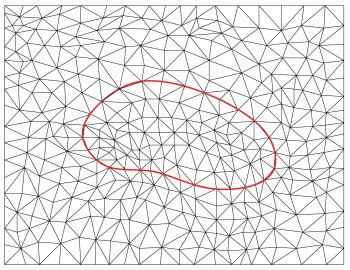
\includegraphics[width=0.4\textwidth]{gfx/immersed_boundary/general_partition_triangle.jpg}\label{fig:grid_f0}}
  \hfil
  \subfloat[unstructured body-fitted grid]{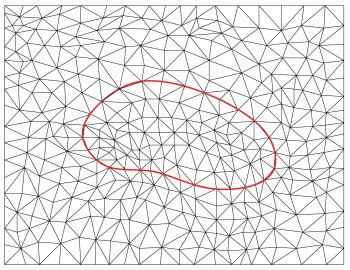
\includegraphics[width=0.4\textwidth]{gfx/immersed_boundary/general_partition_triangle.jpg}\label{fig:grid_f2}}
  \caption{Different types of numerical grids}
\end{figure}

For many fluid problems it is mandatory to solve the equations of motion with respect to complex-shaped geometries \.
The algorithm introduced in section () is not yet suitable for such a scenario.
For instance the simulation inside a spheric geometry is impossible, since the boundaries
do not coincide with the implemented cartesian grid. Nevertheless there exist different approaches to overcome this problem,
which shall be introduced here. \\
The common approach to extend the algorithm would be to use a body-fitted mesh (see figure \ref{fig:grid_f1}),
different advantages and disadvantages arise with this kind of implementation (see \citep{Mittal2005}).
One benefit is a much simpler deployment of the desired boundary condition, due to the overlap of the grid with domain border.
Furthermore a higher accuracy can be achieved \citep{Gornak2013}.
However, using an unstructered grid generates plenty of computational overhead, during and before the execution of a simulation.
The generation of the grid is very complicated in contrast to using a cartesian grid, this can be even more complicated when
considering moving boundaries.
Also solving the finite differenc schemes on a curvilinear coordinate system, leads to more calculations on a single grid point.
The last important aspect is the implementation on the gpu.
Like discussed in section () it is more efficient to use homogenous storage and calculation pattern on a CUDA-device,
the use of unstructured data makes this very difficult.
Altough some attempts exists to solve these difficulties (see i.e. PAP), it is still uncertain if the obtained performance loss would be acceptable.\\
A set of alternative methods, to resolve the problems described above, are so called Immersed Boundary Methods.
The term was first mentioned in (PESKIN 1972), for the simulation of blood flow through a heartvale, but has since then been used for a variety of
methods (MITTAL).  All of them have the idea in common to perform the simulations on a cartesian grid which does not conform to the domain boundary.
To satisfy the desired boundary conditions additional terms are introduced into the equations of motion.
In general one can distinguish between contiuous forcing methods and direct forcing methods.
Continious forcing methods try to mimic the boundary using a localized force which acts on the boundary,
since the surface is tracked by lagrangian points this methods can be well suited for moving boundaries (MITTAL).
One common problem is that continous forcing can arise to stability problem and numerical oscillations in numericial stiff problem (SOURCE).
The direct forcing approach tries to satisfies the boundary condition, by imposing it directly to points near the fluid surface for example
trough an interpolaltion procedure.
Some of the major drawbacks using the IBM is the loss in  spatial accuracy at the boundary, therefore it can be necessary to use a higher grid resolution
compared to a body-fitted mesh.  Futhermore the non-conforming (?) boundaries are more difficult implement.
The benefits of these methods is the use of a cartesian grid, which is much more suited for a gpu-based implementation (see section X).
As a result the overall performance will probably be in the same order as the original algorithm.
In the thesis the Implementation of different Immersed Boundary Methods is seperated into three chapters depending on the boundary condition and application.
This chapter beginns with Implementation of NoSlip-Walls which are the easisest to implement.
The term Immersed Boundary Method is vaguely defined in literature, in this thesis we refer to it with all methods introduced in the following three chapters.


\section{Implemented IBMs}
\subsection{Volume Penalization}
Die Volume-Penalization Methode ermöglicht es, durch einen Kraftterm der auf die einzelnen Fluidzellen wirkt, mit wenig Aufwand Noslip-Ränder zu implementieren.
Das Verfahren wurde in mehreren Publikationen z.B. [bla] erfolgreich verwendet, eine mathematisch exaktere Abhandlung lässt sich z.B. in [bla2] finden.

\begin{wrapfigure}{r}{0.5\textwidth}
  \begin{center}
  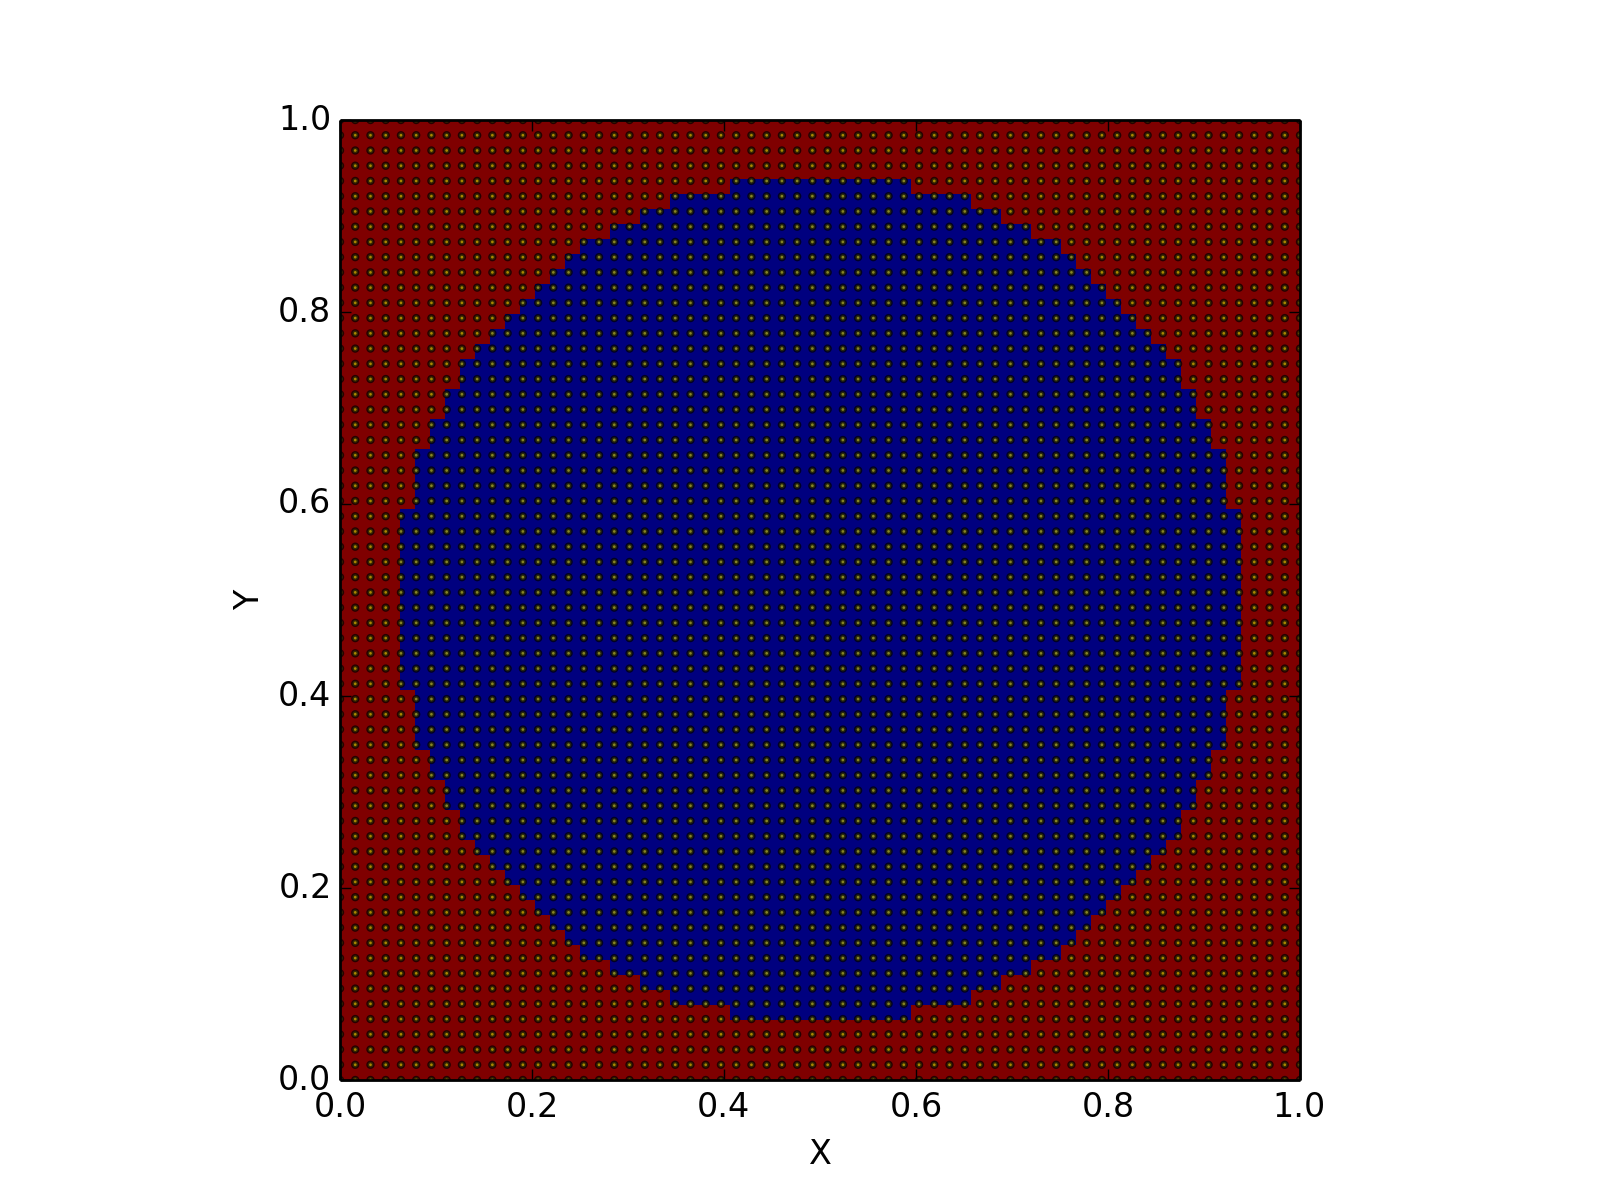
\includegraphics[width=0.5\textwidth]{gfx/immersed_boundary/mask.png}\label{fig:mask_vp}
  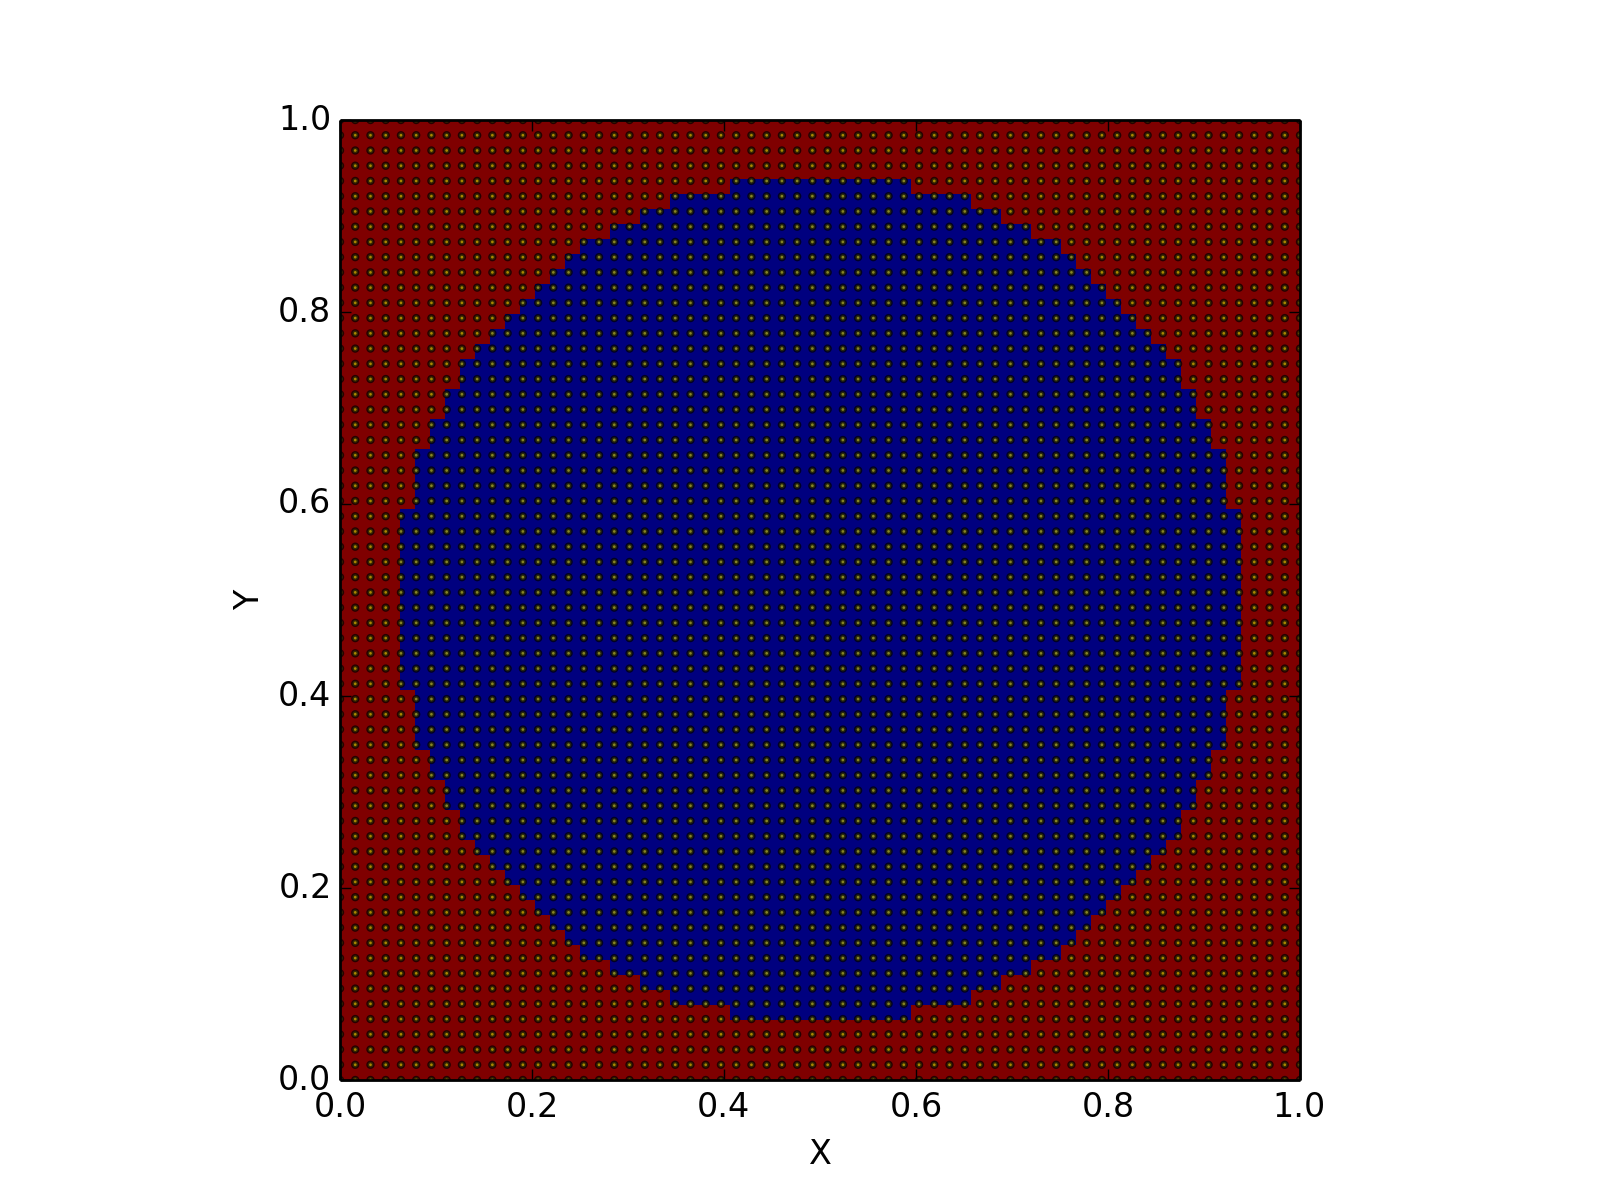
\includegraphics[width=0.5\textwidth]{gfx/immersed_boundary/mask.png}\label{fig:mask_vp}
  \end{center}
  \caption{Maskierungsfunktion $H(x,y,z=const.) = x^2 + y^2 < c$ für einen Zylinder. }
\end{wrapfigure}

Das Volumen wird zunächst in einen Fluidbereich und einen festen Wandbereich, wie in Abb.1 dargestellt, unterteilt. Für die Differenzierung der Bereiche während der Simulation wird  eine Maskierungsfunktion
\begin{align}
H(x, y, z) = \begin{cases}
                    0, & \text{für } \vec{x}(x,y,z) \in Fluid, \\
                    1, & \text{sonst}.
             \end{cases}
\end{align}
verwendet. Als zusätzlicher Kraftterm wird nun eine exponentielle Dämpfung eingeführt die nur auf den Wandbereich des Volumens wirkt.
\begin{align}
\vec{f} = \frac{H(x, y, z)}{\nu}(\vec{v} - \vec{v_0})
\end{align}
Bei $\vec{v_0}$ handelt es sich um die gewünschte Randbedingung, der Kraftterm ist also proportional zur Auslenkung $\vec{v}$ eines Punktes vom gewünschten Ruhezustand.
Die Antwort des Kraftterms wird durch die Dämpfungrate $\nu$ reguliert. Je kleiner $\nu$ desto stärker ist die Dämpfungsrate, allerdings kann der Term
nicht beliebig klein gesetzt werden da die Stabilität für $\nu < dt$ nicht mehr gewährleistet ist [source].
Da für die Lösung der der Geschwindingskeitsfelder mit der Methode der künstliche Kompressibilität  bereits ein sehr kleiner Zeitschritt verwendet wird (s.Abb. X)
kann im Vergleich zu anderen Verfahren wie z.B. (pseudo-spektrale) eine relativ starke Dämpfungsrate verwendet werden.

\subsubsection{Validierung mit MASA}
-validierung mit masa für alle verfahren oben.. cube /evtl zylinder?
-vegl. und argumentation ränder ehh auf null.
-ein beispiel mit vol.pen.

\subsection{Direct Forcing}
\subsection{Volume fraction}
\subsection{Interpolation}
\newpage

\section{Validation}

In order to ensure a correct numerical behaviour of the introduced methods,
a large part of the thesis deals with the numerical validation.
Multiple examples from simple to more complex testcases are introduced in this section.
In general it is necessary to obtain a good evaluation of the numerical truncation error, the numerical stability over longer periods of time
and the fullfilment of the conversation laws, most importantly mass conservation.
Grid convergence studys against theoretical and high-resolution numerical solutions  will be performed
and compared for the different IBMs.


\subsection{Laminar Poiseuille-Flow}
\subsubsection{Theoretical description}

\begin{figure}[!bp]
  \centering
  \includegraphics[width=0.8\textwidth]{gfx/immersed_boundary/val_volpen/poiseuilleflow.png}\label{b}
  \caption{Theoretical setup of the poiseuille-flow channel.}
\end{figure}

%\begin{wrapfigure}{r}{0.5\textwidth}
%  \begin{center}
%      \includegraphics[width=0.48\textwidth]{gfx/immersed_boundary_methods/val_volpen/poiseuilleflow.png}
%   \end{center}
%          \caption{ paxvleb xvle}
%\end{wrapfigure}


The first testcases is the laminar poiseuille-flow, the theoretical setup is presented in figure ().
It consist of two infintiy long planes at $z=h_1$ and $z=h_2$, which are oriented parallel to the xy-plane and the distance $\Delta h = h_2 - h_1$ between them.
Numerically this is realized by using periodic boundaries in xy-direction and no-slip boundaries in z-direction.
The velocity profile results from an external force, given by a  pressure gradient in x-direction, which is introduced into the naviers-stokes equation.
No other forces are present furthermore the flow will be independent of the y coordinate,
hence for the steady state $\partial v_x /\partial t = 0$ the equations of motion can be reduced to:

\begin{align}
\frac{\partial v_x}{\partial t} &= - \frac{\partial p}{\partial x} + \nu \frac{\partial^2 v_x}{\partial z^2} = 0
\end{align}

The equation can simply be integrated twice which yields the solution

\begin{align}
v_x &= \frac{1}{2\nu}\frac{\partial p}{\partial x}z^2 + zc_1 + c_2
\end{align}

Using the noslip-boundary condition $v_x(h_1) = v_x(h_2) = 0$ and furthermore by defining
$A:=\frac{1}{2\nu}\frac{\partial p}{\partial x}$ one obtains the additional conditions

\begin{align}
c_1 &= A\frac{h_1^2 -h_2^2}{h_2 - h_1} = -A(h_1+h_2)\\
c_2 &= A(h_1(h_1 + h_2) - h_1^2) = Ah_1h_2\\
\end{align}

The velocity is than given by the quadratic function

\begin{align}
v_x &= A(z^2 - z(h_1 + h_2) + h_1h_2)
\end{align}

The maximum velocity and postinon can be obtained by simple calculus

\begin{align}
z_{max} &= \frac{h_1+h_2}{2} \wedge v_{max} = A\left(h_1h_2 - \frac{(h_1 + h_2)^2}{4}\right)
\end{align}

and the reynolds number of the system is given by
\begin{align}
    Re &= \frac{v_{max} }{\nu} = \frac{1}{2\nu^2}\pdn[p]{x}\left(h_1h_2 - \frac{(h_1 + h_2)^2}{4}\right)
\end{align}



With the given theoretical solution, the next objective is the comparison
to the default implementation, the volume penalization method and the direct forcing method.
Since we have a flow parallel to the grid  it does not make sence to compare it to the interpolation methods
For the comparision with a theoretical solution it is necessary to ensure that the surface grid points match with the total height $h$ of the channel.
In the default setup the noslip-boundaries are realized with the default implementation, like explained in section ().
For the immersed boundary methdos the upper- and lower boundaries are given by the masking function.
\begin{align}
H(x, y, z) = \begin{cases}
                    0, & \text{for \  }  z < h_2 \lor z>h_1 \\
                    1, & \text{else}.
             \end{cases}
\end{align}

\subsubsection{Test of the Default Implementation}

\begin{figure}[!bp]
    \centering
    %% Creator: Matplotlib, PGF backend
%%
%% To include the figure in your LaTeX document, write
%%   \input{<filename>.pgf}
%%
%% Make sure the required packages are loaded in your preamble
%%   \usepackage{pgf}
%%
%% Figures using additional raster images can only be included by \input if
%% they are in the same directory as the main LaTeX file. For loading figures
%% from other directories you can use the `import` package
%%   \usepackage{import}
%% and then include the figures with
%%   \import{<path to file>}{<filename>.pgf}
%%
%% Matplotlib used the following preamble
%%   \usepackage[utf8x]{inputenc}
%%   \usepackage[T1]{fontenc}
%%
\begingroup%
\makeatletter%
\begin{pgfpicture}%
\pgfpathrectangle{\pgfpointorigin}{\pgfqpoint{4.960630in}{3.065838in}}%
\pgfusepath{use as bounding box, clip}%
\begin{pgfscope}%
\pgfsetbuttcap%
\pgfsetmiterjoin%
\definecolor{currentfill}{rgb}{1.000000,1.000000,1.000000}%
\pgfsetfillcolor{currentfill}%
\pgfsetlinewidth{0.000000pt}%
\definecolor{currentstroke}{rgb}{1.000000,1.000000,1.000000}%
\pgfsetstrokecolor{currentstroke}%
\pgfsetdash{}{0pt}%
\pgfpathmoveto{\pgfqpoint{0.000000in}{0.000000in}}%
\pgfpathlineto{\pgfqpoint{4.960630in}{0.000000in}}%
\pgfpathlineto{\pgfqpoint{4.960630in}{3.065838in}}%
\pgfpathlineto{\pgfqpoint{0.000000in}{3.065838in}}%
\pgfpathclose%
\pgfusepath{fill}%
\end{pgfscope}%
\begin{pgfscope}%
\pgfsetbuttcap%
\pgfsetmiterjoin%
\definecolor{currentfill}{rgb}{1.000000,1.000000,1.000000}%
\pgfsetfillcolor{currentfill}%
\pgfsetlinewidth{0.000000pt}%
\definecolor{currentstroke}{rgb}{0.000000,0.000000,0.000000}%
\pgfsetstrokecolor{currentstroke}%
\pgfsetstrokeopacity{0.000000}%
\pgfsetdash{}{0pt}%
\pgfpathmoveto{\pgfqpoint{0.704753in}{0.497516in}}%
\pgfpathlineto{\pgfqpoint{4.810630in}{0.497516in}}%
\pgfpathlineto{\pgfqpoint{4.810630in}{2.865908in}}%
\pgfpathlineto{\pgfqpoint{0.704753in}{2.865908in}}%
\pgfpathclose%
\pgfusepath{fill}%
\end{pgfscope}%
\begin{pgfscope}%
\pgfpathrectangle{\pgfqpoint{0.704753in}{0.497516in}}{\pgfqpoint{4.105877in}{2.368392in}} %
\pgfusepath{clip}%
\pgfsetrectcap%
\pgfsetroundjoin%
\pgfsetlinewidth{1.003750pt}%
\definecolor{currentstroke}{rgb}{0.894118,0.101961,0.109804}%
\pgfsetstrokecolor{currentstroke}%
\pgfsetdash{}{0pt}%
\pgfpathmoveto{\pgfqpoint{1.079261in}{2.602568in}}%
\pgfpathlineto{\pgfqpoint{4.562262in}{1.846756in}}%
\pgfpathlineto{\pgfqpoint{4.562262in}{1.846756in}}%
\pgfusepath{stroke}%
\end{pgfscope}%
\begin{pgfscope}%
\pgfpathrectangle{\pgfqpoint{0.704753in}{0.497516in}}{\pgfqpoint{4.105877in}{2.368392in}} %
\pgfusepath{clip}%
\pgfsetbuttcap%
\pgfsetroundjoin%
\pgfsetlinewidth{1.003750pt}%
\definecolor{currentstroke}{rgb}{0.215686,0.494118,0.721569}%
\pgfsetstrokecolor{currentstroke}%
\pgfsetdash{{6.000000pt}{6.000000pt}}{0.000000pt}%
\pgfpathmoveto{\pgfqpoint{1.227887in}{1.116849in}}%
\pgfpathlineto{\pgfqpoint{1.999389in}{1.108510in}}%
\pgfpathlineto{\pgfqpoint{2.450688in}{1.171682in}}%
\pgfpathlineto{\pgfqpoint{2.770891in}{1.272260in}}%
\pgfpathlineto{\pgfqpoint{3.019259in}{1.172784in}}%
\pgfpathlineto{\pgfqpoint{3.222190in}{1.147478in}}%
\pgfpathlineto{\pgfqpoint{3.393766in}{1.069301in}}%
\pgfpathlineto{\pgfqpoint{3.542392in}{1.232598in}}%
\pgfpathlineto{\pgfqpoint{3.673490in}{1.074698in}}%
\pgfpathlineto{\pgfqpoint{3.790761in}{1.191798in}}%
\pgfpathlineto{\pgfqpoint{3.896845in}{1.144397in}}%
\pgfpathlineto{\pgfqpoint{3.993692in}{1.202136in}}%
\pgfpathlineto{\pgfqpoint{4.082783in}{0.748560in}}%
\pgfpathlineto{\pgfqpoint{4.165268in}{0.871333in}}%
\pgfpathlineto{\pgfqpoint{4.242060in}{0.871428in}}%
\pgfpathlineto{\pgfqpoint{4.313894in}{0.680827in}}%
\pgfusepath{stroke}%
\end{pgfscope}%
\begin{pgfscope}%
\pgfpathrectangle{\pgfqpoint{0.704753in}{0.497516in}}{\pgfqpoint{4.105877in}{2.368392in}} %
\pgfusepath{clip}%
\pgfsetbuttcap%
\pgfsetmiterjoin%
\definecolor{currentfill}{rgb}{0.215686,0.494118,0.721569}%
\pgfsetfillcolor{currentfill}%
\pgfsetlinewidth{0.501875pt}%
\definecolor{currentstroke}{rgb}{0.000000,0.000000,0.000000}%
\pgfsetstrokecolor{currentstroke}%
\pgfsetdash{}{0pt}%
\pgfsys@defobject{currentmarker}{\pgfqpoint{-0.041667in}{-0.041667in}}{\pgfqpoint{0.041667in}{0.041667in}}{%
\pgfpathmoveto{\pgfqpoint{0.000000in}{0.041667in}}%
\pgfpathlineto{\pgfqpoint{-0.041667in}{-0.041667in}}%
\pgfpathlineto{\pgfqpoint{0.041667in}{-0.041667in}}%
\pgfpathclose%
\pgfusepath{stroke,fill}%
}%
\begin{pgfscope}%
\pgfsys@transformshift{1.227887in}{1.116849in}%
\pgfsys@useobject{currentmarker}{}%
\end{pgfscope}%
\begin{pgfscope}%
\pgfsys@transformshift{1.999389in}{1.108510in}%
\pgfsys@useobject{currentmarker}{}%
\end{pgfscope}%
\begin{pgfscope}%
\pgfsys@transformshift{2.450688in}{1.171682in}%
\pgfsys@useobject{currentmarker}{}%
\end{pgfscope}%
\begin{pgfscope}%
\pgfsys@transformshift{2.770891in}{1.272260in}%
\pgfsys@useobject{currentmarker}{}%
\end{pgfscope}%
\begin{pgfscope}%
\pgfsys@transformshift{3.019259in}{1.172784in}%
\pgfsys@useobject{currentmarker}{}%
\end{pgfscope}%
\begin{pgfscope}%
\pgfsys@transformshift{3.222190in}{1.147478in}%
\pgfsys@useobject{currentmarker}{}%
\end{pgfscope}%
\begin{pgfscope}%
\pgfsys@transformshift{3.393766in}{1.069301in}%
\pgfsys@useobject{currentmarker}{}%
\end{pgfscope}%
\begin{pgfscope}%
\pgfsys@transformshift{3.542392in}{1.232598in}%
\pgfsys@useobject{currentmarker}{}%
\end{pgfscope}%
\begin{pgfscope}%
\pgfsys@transformshift{3.673490in}{1.074698in}%
\pgfsys@useobject{currentmarker}{}%
\end{pgfscope}%
\begin{pgfscope}%
\pgfsys@transformshift{3.790761in}{1.191798in}%
\pgfsys@useobject{currentmarker}{}%
\end{pgfscope}%
\begin{pgfscope}%
\pgfsys@transformshift{3.896845in}{1.144397in}%
\pgfsys@useobject{currentmarker}{}%
\end{pgfscope}%
\begin{pgfscope}%
\pgfsys@transformshift{3.993692in}{1.202136in}%
\pgfsys@useobject{currentmarker}{}%
\end{pgfscope}%
\begin{pgfscope}%
\pgfsys@transformshift{4.082783in}{0.748560in}%
\pgfsys@useobject{currentmarker}{}%
\end{pgfscope}%
\begin{pgfscope}%
\pgfsys@transformshift{4.165268in}{0.871333in}%
\pgfsys@useobject{currentmarker}{}%
\end{pgfscope}%
\begin{pgfscope}%
\pgfsys@transformshift{4.242060in}{0.871428in}%
\pgfsys@useobject{currentmarker}{}%
\end{pgfscope}%
\begin{pgfscope}%
\pgfsys@transformshift{4.313894in}{0.680827in}%
\pgfsys@useobject{currentmarker}{}%
\end{pgfscope}%
\end{pgfscope}%
\begin{pgfscope}%
\pgfpathrectangle{\pgfqpoint{0.704753in}{0.497516in}}{\pgfqpoint{4.105877in}{2.368392in}} %
\pgfusepath{clip}%
\pgfsetbuttcap%
\pgfsetroundjoin%
\pgfsetlinewidth{1.003750pt}%
\definecolor{currentstroke}{rgb}{0.301961,0.686275,0.290196}%
\pgfsetstrokecolor{currentstroke}%
\pgfsetdash{{6.000000pt}{6.000000pt}}{0.000000pt}%
\pgfpathmoveto{\pgfqpoint{1.227887in}{2.570216in}}%
\pgfpathlineto{\pgfqpoint{1.999389in}{2.406661in}}%
\pgfpathlineto{\pgfqpoint{2.450688in}{2.300419in}}%
\pgfpathlineto{\pgfqpoint{2.770891in}{2.220411in}}%
\pgfpathlineto{\pgfqpoint{3.019259in}{2.170731in}}%
\pgfpathlineto{\pgfqpoint{3.222190in}{2.128775in}}%
\pgfpathlineto{\pgfqpoint{3.393766in}{2.094708in}}%
\pgfpathlineto{\pgfqpoint{3.542392in}{2.060246in}}%
\pgfpathlineto{\pgfqpoint{3.673490in}{2.026097in}}%
\pgfpathlineto{\pgfqpoint{3.790761in}{2.006229in}}%
\pgfpathlineto{\pgfqpoint{3.896845in}{1.978424in}}%
\pgfpathlineto{\pgfqpoint{3.993692in}{1.953876in}}%
\pgfpathlineto{\pgfqpoint{4.082783in}{1.944457in}}%
\pgfpathlineto{\pgfqpoint{4.165268in}{1.922840in}}%
\pgfpathlineto{\pgfqpoint{4.242060in}{1.903072in}}%
\pgfpathlineto{\pgfqpoint{4.313894in}{1.893257in}}%
\pgfusepath{stroke}%
\end{pgfscope}%
\begin{pgfscope}%
\pgfpathrectangle{\pgfqpoint{0.704753in}{0.497516in}}{\pgfqpoint{4.105877in}{2.368392in}} %
\pgfusepath{clip}%
\pgfsetbuttcap%
\pgfsetmiterjoin%
\definecolor{currentfill}{rgb}{0.301961,0.686275,0.290196}%
\pgfsetfillcolor{currentfill}%
\pgfsetlinewidth{0.501875pt}%
\definecolor{currentstroke}{rgb}{0.000000,0.000000,0.000000}%
\pgfsetstrokecolor{currentstroke}%
\pgfsetdash{}{0pt}%
\pgfsys@defobject{currentmarker}{\pgfqpoint{-0.036084in}{-0.041667in}}{\pgfqpoint{0.036084in}{0.041667in}}{%
\pgfpathmoveto{\pgfqpoint{0.000000in}{0.041667in}}%
\pgfpathlineto{\pgfqpoint{-0.036084in}{0.020833in}}%
\pgfpathlineto{\pgfqpoint{-0.036084in}{-0.020833in}}%
\pgfpathlineto{\pgfqpoint{-0.000000in}{-0.041667in}}%
\pgfpathlineto{\pgfqpoint{0.036084in}{-0.020833in}}%
\pgfpathlineto{\pgfqpoint{0.036084in}{0.020833in}}%
\pgfpathclose%
\pgfusepath{stroke,fill}%
}%
\begin{pgfscope}%
\pgfsys@transformshift{1.227887in}{2.570216in}%
\pgfsys@useobject{currentmarker}{}%
\end{pgfscope}%
\begin{pgfscope}%
\pgfsys@transformshift{1.999389in}{2.406661in}%
\pgfsys@useobject{currentmarker}{}%
\end{pgfscope}%
\begin{pgfscope}%
\pgfsys@transformshift{2.450688in}{2.300419in}%
\pgfsys@useobject{currentmarker}{}%
\end{pgfscope}%
\begin{pgfscope}%
\pgfsys@transformshift{2.770891in}{2.220411in}%
\pgfsys@useobject{currentmarker}{}%
\end{pgfscope}%
\begin{pgfscope}%
\pgfsys@transformshift{3.019259in}{2.170731in}%
\pgfsys@useobject{currentmarker}{}%
\end{pgfscope}%
\begin{pgfscope}%
\pgfsys@transformshift{3.222190in}{2.128775in}%
\pgfsys@useobject{currentmarker}{}%
\end{pgfscope}%
\begin{pgfscope}%
\pgfsys@transformshift{3.393766in}{2.094708in}%
\pgfsys@useobject{currentmarker}{}%
\end{pgfscope}%
\begin{pgfscope}%
\pgfsys@transformshift{3.542392in}{2.060246in}%
\pgfsys@useobject{currentmarker}{}%
\end{pgfscope}%
\begin{pgfscope}%
\pgfsys@transformshift{3.673490in}{2.026097in}%
\pgfsys@useobject{currentmarker}{}%
\end{pgfscope}%
\begin{pgfscope}%
\pgfsys@transformshift{3.790761in}{2.006229in}%
\pgfsys@useobject{currentmarker}{}%
\end{pgfscope}%
\begin{pgfscope}%
\pgfsys@transformshift{3.896845in}{1.978424in}%
\pgfsys@useobject{currentmarker}{}%
\end{pgfscope}%
\begin{pgfscope}%
\pgfsys@transformshift{3.993692in}{1.953876in}%
\pgfsys@useobject{currentmarker}{}%
\end{pgfscope}%
\begin{pgfscope}%
\pgfsys@transformshift{4.082783in}{1.944457in}%
\pgfsys@useobject{currentmarker}{}%
\end{pgfscope}%
\begin{pgfscope}%
\pgfsys@transformshift{4.165268in}{1.922840in}%
\pgfsys@useobject{currentmarker}{}%
\end{pgfscope}%
\begin{pgfscope}%
\pgfsys@transformshift{4.242060in}{1.903072in}%
\pgfsys@useobject{currentmarker}{}%
\end{pgfscope}%
\begin{pgfscope}%
\pgfsys@transformshift{4.313894in}{1.893257in}%
\pgfsys@useobject{currentmarker}{}%
\end{pgfscope}%
\end{pgfscope}%
\begin{pgfscope}%
\pgfsetrectcap%
\pgfsetmiterjoin%
\pgfsetlinewidth{1.003750pt}%
\definecolor{currentstroke}{rgb}{0.000000,0.000000,0.000000}%
\pgfsetstrokecolor{currentstroke}%
\pgfsetdash{}{0pt}%
\pgfpathmoveto{\pgfqpoint{0.704753in}{2.865908in}}%
\pgfpathlineto{\pgfqpoint{4.810630in}{2.865908in}}%
\pgfusepath{stroke}%
\end{pgfscope}%
\begin{pgfscope}%
\pgfsetrectcap%
\pgfsetmiterjoin%
\pgfsetlinewidth{1.003750pt}%
\definecolor{currentstroke}{rgb}{0.000000,0.000000,0.000000}%
\pgfsetstrokecolor{currentstroke}%
\pgfsetdash{}{0pt}%
\pgfpathmoveto{\pgfqpoint{4.810630in}{0.497516in}}%
\pgfpathlineto{\pgfqpoint{4.810630in}{2.865908in}}%
\pgfusepath{stroke}%
\end{pgfscope}%
\begin{pgfscope}%
\pgfsetrectcap%
\pgfsetmiterjoin%
\pgfsetlinewidth{1.003750pt}%
\definecolor{currentstroke}{rgb}{0.000000,0.000000,0.000000}%
\pgfsetstrokecolor{currentstroke}%
\pgfsetdash{}{0pt}%
\pgfpathmoveto{\pgfqpoint{0.704753in}{0.497516in}}%
\pgfpathlineto{\pgfqpoint{4.810630in}{0.497516in}}%
\pgfusepath{stroke}%
\end{pgfscope}%
\begin{pgfscope}%
\pgfsetrectcap%
\pgfsetmiterjoin%
\pgfsetlinewidth{1.003750pt}%
\definecolor{currentstroke}{rgb}{0.000000,0.000000,0.000000}%
\pgfsetstrokecolor{currentstroke}%
\pgfsetdash{}{0pt}%
\pgfpathmoveto{\pgfqpoint{0.704753in}{0.497516in}}%
\pgfpathlineto{\pgfqpoint{0.704753in}{2.865908in}}%
\pgfusepath{stroke}%
\end{pgfscope}%
\begin{pgfscope}%
\pgfpathrectangle{\pgfqpoint{0.704753in}{0.497516in}}{\pgfqpoint{4.105877in}{2.368392in}} %
\pgfusepath{clip}%
\pgfsetbuttcap%
\pgfsetroundjoin%
\pgfsetlinewidth{0.501875pt}%
\definecolor{currentstroke}{rgb}{0.000000,0.000000,0.000000}%
\pgfsetstrokecolor{currentstroke}%
\pgfsetdash{{1.000000pt}{3.000000pt}}{0.000000pt}%
\pgfpathmoveto{\pgfqpoint{1.476255in}{0.497516in}}%
\pgfpathlineto{\pgfqpoint{1.476255in}{2.865908in}}%
\pgfusepath{stroke}%
\end{pgfscope}%
\begin{pgfscope}%
\pgfsetbuttcap%
\pgfsetroundjoin%
\definecolor{currentfill}{rgb}{0.000000,0.000000,0.000000}%
\pgfsetfillcolor{currentfill}%
\pgfsetlinewidth{0.501875pt}%
\definecolor{currentstroke}{rgb}{0.000000,0.000000,0.000000}%
\pgfsetstrokecolor{currentstroke}%
\pgfsetdash{}{0pt}%
\pgfsys@defobject{currentmarker}{\pgfqpoint{0.000000in}{0.000000in}}{\pgfqpoint{0.000000in}{0.055556in}}{%
\pgfpathmoveto{\pgfqpoint{0.000000in}{0.000000in}}%
\pgfpathlineto{\pgfqpoint{0.000000in}{0.055556in}}%
\pgfusepath{stroke,fill}%
}%
\begin{pgfscope}%
\pgfsys@transformshift{1.476255in}{0.497516in}%
\pgfsys@useobject{currentmarker}{}%
\end{pgfscope}%
\end{pgfscope}%
\begin{pgfscope}%
\pgfsetbuttcap%
\pgfsetroundjoin%
\definecolor{currentfill}{rgb}{0.000000,0.000000,0.000000}%
\pgfsetfillcolor{currentfill}%
\pgfsetlinewidth{0.501875pt}%
\definecolor{currentstroke}{rgb}{0.000000,0.000000,0.000000}%
\pgfsetstrokecolor{currentstroke}%
\pgfsetdash{}{0pt}%
\pgfsys@defobject{currentmarker}{\pgfqpoint{0.000000in}{-0.055556in}}{\pgfqpoint{0.000000in}{0.000000in}}{%
\pgfpathmoveto{\pgfqpoint{0.000000in}{0.000000in}}%
\pgfpathlineto{\pgfqpoint{0.000000in}{-0.055556in}}%
\pgfusepath{stroke,fill}%
}%
\begin{pgfscope}%
\pgfsys@transformshift{1.476255in}{2.865908in}%
\pgfsys@useobject{currentmarker}{}%
\end{pgfscope}%
\end{pgfscope}%
\begin{pgfscope}%
\pgftext[x=1.476255in,y=0.441961in,,top]{\rmfamily\fontsize{8.000000}{9.600000}\selectfont \(\displaystyle 10^{1}\)}%
\end{pgfscope}%
\begin{pgfscope}%
\pgfpathrectangle{\pgfqpoint{0.704753in}{0.497516in}}{\pgfqpoint{4.105877in}{2.368392in}} %
\pgfusepath{clip}%
\pgfsetbuttcap%
\pgfsetroundjoin%
\pgfsetlinewidth{0.501875pt}%
\definecolor{currentstroke}{rgb}{0.000000,0.000000,0.000000}%
\pgfsetstrokecolor{currentstroke}%
\pgfsetdash{{1.000000pt}{3.000000pt}}{0.000000pt}%
\pgfpathmoveto{\pgfqpoint{4.039129in}{0.497516in}}%
\pgfpathlineto{\pgfqpoint{4.039129in}{2.865908in}}%
\pgfusepath{stroke}%
\end{pgfscope}%
\begin{pgfscope}%
\pgfsetbuttcap%
\pgfsetroundjoin%
\definecolor{currentfill}{rgb}{0.000000,0.000000,0.000000}%
\pgfsetfillcolor{currentfill}%
\pgfsetlinewidth{0.501875pt}%
\definecolor{currentstroke}{rgb}{0.000000,0.000000,0.000000}%
\pgfsetstrokecolor{currentstroke}%
\pgfsetdash{}{0pt}%
\pgfsys@defobject{currentmarker}{\pgfqpoint{0.000000in}{0.000000in}}{\pgfqpoint{0.000000in}{0.055556in}}{%
\pgfpathmoveto{\pgfqpoint{0.000000in}{0.000000in}}%
\pgfpathlineto{\pgfqpoint{0.000000in}{0.055556in}}%
\pgfusepath{stroke,fill}%
}%
\begin{pgfscope}%
\pgfsys@transformshift{4.039129in}{0.497516in}%
\pgfsys@useobject{currentmarker}{}%
\end{pgfscope}%
\end{pgfscope}%
\begin{pgfscope}%
\pgfsetbuttcap%
\pgfsetroundjoin%
\definecolor{currentfill}{rgb}{0.000000,0.000000,0.000000}%
\pgfsetfillcolor{currentfill}%
\pgfsetlinewidth{0.501875pt}%
\definecolor{currentstroke}{rgb}{0.000000,0.000000,0.000000}%
\pgfsetstrokecolor{currentstroke}%
\pgfsetdash{}{0pt}%
\pgfsys@defobject{currentmarker}{\pgfqpoint{0.000000in}{-0.055556in}}{\pgfqpoint{0.000000in}{0.000000in}}{%
\pgfpathmoveto{\pgfqpoint{0.000000in}{0.000000in}}%
\pgfpathlineto{\pgfqpoint{0.000000in}{-0.055556in}}%
\pgfusepath{stroke,fill}%
}%
\begin{pgfscope}%
\pgfsys@transformshift{4.039129in}{2.865908in}%
\pgfsys@useobject{currentmarker}{}%
\end{pgfscope}%
\end{pgfscope}%
\begin{pgfscope}%
\pgftext[x=4.039129in,y=0.441961in,,top]{\rmfamily\fontsize{8.000000}{9.600000}\selectfont \(\displaystyle 10^{2}\)}%
\end{pgfscope}%
\begin{pgfscope}%
\pgfsetbuttcap%
\pgfsetroundjoin%
\definecolor{currentfill}{rgb}{0.000000,0.000000,0.000000}%
\pgfsetfillcolor{currentfill}%
\pgfsetlinewidth{0.501875pt}%
\definecolor{currentstroke}{rgb}{0.000000,0.000000,0.000000}%
\pgfsetstrokecolor{currentstroke}%
\pgfsetdash{}{0pt}%
\pgfsys@defobject{currentmarker}{\pgfqpoint{0.000000in}{0.000000in}}{\pgfqpoint{0.000000in}{0.027778in}}{%
\pgfpathmoveto{\pgfqpoint{0.000000in}{0.000000in}}%
\pgfpathlineto{\pgfqpoint{0.000000in}{0.027778in}}%
\pgfusepath{stroke,fill}%
}%
\begin{pgfscope}%
\pgfsys@transformshift{0.704753in}{0.497516in}%
\pgfsys@useobject{currentmarker}{}%
\end{pgfscope}%
\end{pgfscope}%
\begin{pgfscope}%
\pgfsetbuttcap%
\pgfsetroundjoin%
\definecolor{currentfill}{rgb}{0.000000,0.000000,0.000000}%
\pgfsetfillcolor{currentfill}%
\pgfsetlinewidth{0.501875pt}%
\definecolor{currentstroke}{rgb}{0.000000,0.000000,0.000000}%
\pgfsetstrokecolor{currentstroke}%
\pgfsetdash{}{0pt}%
\pgfsys@defobject{currentmarker}{\pgfqpoint{0.000000in}{-0.027778in}}{\pgfqpoint{0.000000in}{0.000000in}}{%
\pgfpathmoveto{\pgfqpoint{0.000000in}{0.000000in}}%
\pgfpathlineto{\pgfqpoint{0.000000in}{-0.027778in}}%
\pgfusepath{stroke,fill}%
}%
\begin{pgfscope}%
\pgfsys@transformshift{0.704753in}{2.865908in}%
\pgfsys@useobject{currentmarker}{}%
\end{pgfscope}%
\end{pgfscope}%
\begin{pgfscope}%
\pgfsetbuttcap%
\pgfsetroundjoin%
\definecolor{currentfill}{rgb}{0.000000,0.000000,0.000000}%
\pgfsetfillcolor{currentfill}%
\pgfsetlinewidth{0.501875pt}%
\definecolor{currentstroke}{rgb}{0.000000,0.000000,0.000000}%
\pgfsetstrokecolor{currentstroke}%
\pgfsetdash{}{0pt}%
\pgfsys@defobject{currentmarker}{\pgfqpoint{0.000000in}{0.000000in}}{\pgfqpoint{0.000000in}{0.027778in}}{%
\pgfpathmoveto{\pgfqpoint{0.000000in}{0.000000in}}%
\pgfpathlineto{\pgfqpoint{0.000000in}{0.027778in}}%
\pgfusepath{stroke,fill}%
}%
\begin{pgfscope}%
\pgfsys@transformshift{0.907685in}{0.497516in}%
\pgfsys@useobject{currentmarker}{}%
\end{pgfscope}%
\end{pgfscope}%
\begin{pgfscope}%
\pgfsetbuttcap%
\pgfsetroundjoin%
\definecolor{currentfill}{rgb}{0.000000,0.000000,0.000000}%
\pgfsetfillcolor{currentfill}%
\pgfsetlinewidth{0.501875pt}%
\definecolor{currentstroke}{rgb}{0.000000,0.000000,0.000000}%
\pgfsetstrokecolor{currentstroke}%
\pgfsetdash{}{0pt}%
\pgfsys@defobject{currentmarker}{\pgfqpoint{0.000000in}{-0.027778in}}{\pgfqpoint{0.000000in}{0.000000in}}{%
\pgfpathmoveto{\pgfqpoint{0.000000in}{0.000000in}}%
\pgfpathlineto{\pgfqpoint{0.000000in}{-0.027778in}}%
\pgfusepath{stroke,fill}%
}%
\begin{pgfscope}%
\pgfsys@transformshift{0.907685in}{2.865908in}%
\pgfsys@useobject{currentmarker}{}%
\end{pgfscope}%
\end{pgfscope}%
\begin{pgfscope}%
\pgfsetbuttcap%
\pgfsetroundjoin%
\definecolor{currentfill}{rgb}{0.000000,0.000000,0.000000}%
\pgfsetfillcolor{currentfill}%
\pgfsetlinewidth{0.501875pt}%
\definecolor{currentstroke}{rgb}{0.000000,0.000000,0.000000}%
\pgfsetstrokecolor{currentstroke}%
\pgfsetdash{}{0pt}%
\pgfsys@defobject{currentmarker}{\pgfqpoint{0.000000in}{0.000000in}}{\pgfqpoint{0.000000in}{0.027778in}}{%
\pgfpathmoveto{\pgfqpoint{0.000000in}{0.000000in}}%
\pgfpathlineto{\pgfqpoint{0.000000in}{0.027778in}}%
\pgfusepath{stroke,fill}%
}%
\begin{pgfscope}%
\pgfsys@transformshift{1.079261in}{0.497516in}%
\pgfsys@useobject{currentmarker}{}%
\end{pgfscope}%
\end{pgfscope}%
\begin{pgfscope}%
\pgfsetbuttcap%
\pgfsetroundjoin%
\definecolor{currentfill}{rgb}{0.000000,0.000000,0.000000}%
\pgfsetfillcolor{currentfill}%
\pgfsetlinewidth{0.501875pt}%
\definecolor{currentstroke}{rgb}{0.000000,0.000000,0.000000}%
\pgfsetstrokecolor{currentstroke}%
\pgfsetdash{}{0pt}%
\pgfsys@defobject{currentmarker}{\pgfqpoint{0.000000in}{-0.027778in}}{\pgfqpoint{0.000000in}{0.000000in}}{%
\pgfpathmoveto{\pgfqpoint{0.000000in}{0.000000in}}%
\pgfpathlineto{\pgfqpoint{0.000000in}{-0.027778in}}%
\pgfusepath{stroke,fill}%
}%
\begin{pgfscope}%
\pgfsys@transformshift{1.079261in}{2.865908in}%
\pgfsys@useobject{currentmarker}{}%
\end{pgfscope}%
\end{pgfscope}%
\begin{pgfscope}%
\pgfsetbuttcap%
\pgfsetroundjoin%
\definecolor{currentfill}{rgb}{0.000000,0.000000,0.000000}%
\pgfsetfillcolor{currentfill}%
\pgfsetlinewidth{0.501875pt}%
\definecolor{currentstroke}{rgb}{0.000000,0.000000,0.000000}%
\pgfsetstrokecolor{currentstroke}%
\pgfsetdash{}{0pt}%
\pgfsys@defobject{currentmarker}{\pgfqpoint{0.000000in}{0.000000in}}{\pgfqpoint{0.000000in}{0.027778in}}{%
\pgfpathmoveto{\pgfqpoint{0.000000in}{0.000000in}}%
\pgfpathlineto{\pgfqpoint{0.000000in}{0.027778in}}%
\pgfusepath{stroke,fill}%
}%
\begin{pgfscope}%
\pgfsys@transformshift{1.227887in}{0.497516in}%
\pgfsys@useobject{currentmarker}{}%
\end{pgfscope}%
\end{pgfscope}%
\begin{pgfscope}%
\pgfsetbuttcap%
\pgfsetroundjoin%
\definecolor{currentfill}{rgb}{0.000000,0.000000,0.000000}%
\pgfsetfillcolor{currentfill}%
\pgfsetlinewidth{0.501875pt}%
\definecolor{currentstroke}{rgb}{0.000000,0.000000,0.000000}%
\pgfsetstrokecolor{currentstroke}%
\pgfsetdash{}{0pt}%
\pgfsys@defobject{currentmarker}{\pgfqpoint{0.000000in}{-0.027778in}}{\pgfqpoint{0.000000in}{0.000000in}}{%
\pgfpathmoveto{\pgfqpoint{0.000000in}{0.000000in}}%
\pgfpathlineto{\pgfqpoint{0.000000in}{-0.027778in}}%
\pgfusepath{stroke,fill}%
}%
\begin{pgfscope}%
\pgfsys@transformshift{1.227887in}{2.865908in}%
\pgfsys@useobject{currentmarker}{}%
\end{pgfscope}%
\end{pgfscope}%
\begin{pgfscope}%
\pgfsetbuttcap%
\pgfsetroundjoin%
\definecolor{currentfill}{rgb}{0.000000,0.000000,0.000000}%
\pgfsetfillcolor{currentfill}%
\pgfsetlinewidth{0.501875pt}%
\definecolor{currentstroke}{rgb}{0.000000,0.000000,0.000000}%
\pgfsetstrokecolor{currentstroke}%
\pgfsetdash{}{0pt}%
\pgfsys@defobject{currentmarker}{\pgfqpoint{0.000000in}{0.000000in}}{\pgfqpoint{0.000000in}{0.027778in}}{%
\pgfpathmoveto{\pgfqpoint{0.000000in}{0.000000in}}%
\pgfpathlineto{\pgfqpoint{0.000000in}{0.027778in}}%
\pgfusepath{stroke,fill}%
}%
\begin{pgfscope}%
\pgfsys@transformshift{1.358984in}{0.497516in}%
\pgfsys@useobject{currentmarker}{}%
\end{pgfscope}%
\end{pgfscope}%
\begin{pgfscope}%
\pgfsetbuttcap%
\pgfsetroundjoin%
\definecolor{currentfill}{rgb}{0.000000,0.000000,0.000000}%
\pgfsetfillcolor{currentfill}%
\pgfsetlinewidth{0.501875pt}%
\definecolor{currentstroke}{rgb}{0.000000,0.000000,0.000000}%
\pgfsetstrokecolor{currentstroke}%
\pgfsetdash{}{0pt}%
\pgfsys@defobject{currentmarker}{\pgfqpoint{0.000000in}{-0.027778in}}{\pgfqpoint{0.000000in}{0.000000in}}{%
\pgfpathmoveto{\pgfqpoint{0.000000in}{0.000000in}}%
\pgfpathlineto{\pgfqpoint{0.000000in}{-0.027778in}}%
\pgfusepath{stroke,fill}%
}%
\begin{pgfscope}%
\pgfsys@transformshift{1.358984in}{2.865908in}%
\pgfsys@useobject{currentmarker}{}%
\end{pgfscope}%
\end{pgfscope}%
\begin{pgfscope}%
\pgfsetbuttcap%
\pgfsetroundjoin%
\definecolor{currentfill}{rgb}{0.000000,0.000000,0.000000}%
\pgfsetfillcolor{currentfill}%
\pgfsetlinewidth{0.501875pt}%
\definecolor{currentstroke}{rgb}{0.000000,0.000000,0.000000}%
\pgfsetstrokecolor{currentstroke}%
\pgfsetdash{}{0pt}%
\pgfsys@defobject{currentmarker}{\pgfqpoint{0.000000in}{0.000000in}}{\pgfqpoint{0.000000in}{0.027778in}}{%
\pgfpathmoveto{\pgfqpoint{0.000000in}{0.000000in}}%
\pgfpathlineto{\pgfqpoint{0.000000in}{0.027778in}}%
\pgfusepath{stroke,fill}%
}%
\begin{pgfscope}%
\pgfsys@transformshift{2.247757in}{0.497516in}%
\pgfsys@useobject{currentmarker}{}%
\end{pgfscope}%
\end{pgfscope}%
\begin{pgfscope}%
\pgfsetbuttcap%
\pgfsetroundjoin%
\definecolor{currentfill}{rgb}{0.000000,0.000000,0.000000}%
\pgfsetfillcolor{currentfill}%
\pgfsetlinewidth{0.501875pt}%
\definecolor{currentstroke}{rgb}{0.000000,0.000000,0.000000}%
\pgfsetstrokecolor{currentstroke}%
\pgfsetdash{}{0pt}%
\pgfsys@defobject{currentmarker}{\pgfqpoint{0.000000in}{-0.027778in}}{\pgfqpoint{0.000000in}{0.000000in}}{%
\pgfpathmoveto{\pgfqpoint{0.000000in}{0.000000in}}%
\pgfpathlineto{\pgfqpoint{0.000000in}{-0.027778in}}%
\pgfusepath{stroke,fill}%
}%
\begin{pgfscope}%
\pgfsys@transformshift{2.247757in}{2.865908in}%
\pgfsys@useobject{currentmarker}{}%
\end{pgfscope}%
\end{pgfscope}%
\begin{pgfscope}%
\pgfsetbuttcap%
\pgfsetroundjoin%
\definecolor{currentfill}{rgb}{0.000000,0.000000,0.000000}%
\pgfsetfillcolor{currentfill}%
\pgfsetlinewidth{0.501875pt}%
\definecolor{currentstroke}{rgb}{0.000000,0.000000,0.000000}%
\pgfsetstrokecolor{currentstroke}%
\pgfsetdash{}{0pt}%
\pgfsys@defobject{currentmarker}{\pgfqpoint{0.000000in}{0.000000in}}{\pgfqpoint{0.000000in}{0.027778in}}{%
\pgfpathmoveto{\pgfqpoint{0.000000in}{0.000000in}}%
\pgfpathlineto{\pgfqpoint{0.000000in}{0.027778in}}%
\pgfusepath{stroke,fill}%
}%
\begin{pgfscope}%
\pgfsys@transformshift{2.699057in}{0.497516in}%
\pgfsys@useobject{currentmarker}{}%
\end{pgfscope}%
\end{pgfscope}%
\begin{pgfscope}%
\pgfsetbuttcap%
\pgfsetroundjoin%
\definecolor{currentfill}{rgb}{0.000000,0.000000,0.000000}%
\pgfsetfillcolor{currentfill}%
\pgfsetlinewidth{0.501875pt}%
\definecolor{currentstroke}{rgb}{0.000000,0.000000,0.000000}%
\pgfsetstrokecolor{currentstroke}%
\pgfsetdash{}{0pt}%
\pgfsys@defobject{currentmarker}{\pgfqpoint{0.000000in}{-0.027778in}}{\pgfqpoint{0.000000in}{0.000000in}}{%
\pgfpathmoveto{\pgfqpoint{0.000000in}{0.000000in}}%
\pgfpathlineto{\pgfqpoint{0.000000in}{-0.027778in}}%
\pgfusepath{stroke,fill}%
}%
\begin{pgfscope}%
\pgfsys@transformshift{2.699057in}{2.865908in}%
\pgfsys@useobject{currentmarker}{}%
\end{pgfscope}%
\end{pgfscope}%
\begin{pgfscope}%
\pgfsetbuttcap%
\pgfsetroundjoin%
\definecolor{currentfill}{rgb}{0.000000,0.000000,0.000000}%
\pgfsetfillcolor{currentfill}%
\pgfsetlinewidth{0.501875pt}%
\definecolor{currentstroke}{rgb}{0.000000,0.000000,0.000000}%
\pgfsetstrokecolor{currentstroke}%
\pgfsetdash{}{0pt}%
\pgfsys@defobject{currentmarker}{\pgfqpoint{0.000000in}{0.000000in}}{\pgfqpoint{0.000000in}{0.027778in}}{%
\pgfpathmoveto{\pgfqpoint{0.000000in}{0.000000in}}%
\pgfpathlineto{\pgfqpoint{0.000000in}{0.027778in}}%
\pgfusepath{stroke,fill}%
}%
\begin{pgfscope}%
\pgfsys@transformshift{3.019259in}{0.497516in}%
\pgfsys@useobject{currentmarker}{}%
\end{pgfscope}%
\end{pgfscope}%
\begin{pgfscope}%
\pgfsetbuttcap%
\pgfsetroundjoin%
\definecolor{currentfill}{rgb}{0.000000,0.000000,0.000000}%
\pgfsetfillcolor{currentfill}%
\pgfsetlinewidth{0.501875pt}%
\definecolor{currentstroke}{rgb}{0.000000,0.000000,0.000000}%
\pgfsetstrokecolor{currentstroke}%
\pgfsetdash{}{0pt}%
\pgfsys@defobject{currentmarker}{\pgfqpoint{0.000000in}{-0.027778in}}{\pgfqpoint{0.000000in}{0.000000in}}{%
\pgfpathmoveto{\pgfqpoint{0.000000in}{0.000000in}}%
\pgfpathlineto{\pgfqpoint{0.000000in}{-0.027778in}}%
\pgfusepath{stroke,fill}%
}%
\begin{pgfscope}%
\pgfsys@transformshift{3.019259in}{2.865908in}%
\pgfsys@useobject{currentmarker}{}%
\end{pgfscope}%
\end{pgfscope}%
\begin{pgfscope}%
\pgfsetbuttcap%
\pgfsetroundjoin%
\definecolor{currentfill}{rgb}{0.000000,0.000000,0.000000}%
\pgfsetfillcolor{currentfill}%
\pgfsetlinewidth{0.501875pt}%
\definecolor{currentstroke}{rgb}{0.000000,0.000000,0.000000}%
\pgfsetstrokecolor{currentstroke}%
\pgfsetdash{}{0pt}%
\pgfsys@defobject{currentmarker}{\pgfqpoint{0.000000in}{0.000000in}}{\pgfqpoint{0.000000in}{0.027778in}}{%
\pgfpathmoveto{\pgfqpoint{0.000000in}{0.000000in}}%
\pgfpathlineto{\pgfqpoint{0.000000in}{0.027778in}}%
\pgfusepath{stroke,fill}%
}%
\begin{pgfscope}%
\pgfsys@transformshift{3.267627in}{0.497516in}%
\pgfsys@useobject{currentmarker}{}%
\end{pgfscope}%
\end{pgfscope}%
\begin{pgfscope}%
\pgfsetbuttcap%
\pgfsetroundjoin%
\definecolor{currentfill}{rgb}{0.000000,0.000000,0.000000}%
\pgfsetfillcolor{currentfill}%
\pgfsetlinewidth{0.501875pt}%
\definecolor{currentstroke}{rgb}{0.000000,0.000000,0.000000}%
\pgfsetstrokecolor{currentstroke}%
\pgfsetdash{}{0pt}%
\pgfsys@defobject{currentmarker}{\pgfqpoint{0.000000in}{-0.027778in}}{\pgfqpoint{0.000000in}{0.000000in}}{%
\pgfpathmoveto{\pgfqpoint{0.000000in}{0.000000in}}%
\pgfpathlineto{\pgfqpoint{0.000000in}{-0.027778in}}%
\pgfusepath{stroke,fill}%
}%
\begin{pgfscope}%
\pgfsys@transformshift{3.267627in}{2.865908in}%
\pgfsys@useobject{currentmarker}{}%
\end{pgfscope}%
\end{pgfscope}%
\begin{pgfscope}%
\pgfsetbuttcap%
\pgfsetroundjoin%
\definecolor{currentfill}{rgb}{0.000000,0.000000,0.000000}%
\pgfsetfillcolor{currentfill}%
\pgfsetlinewidth{0.501875pt}%
\definecolor{currentstroke}{rgb}{0.000000,0.000000,0.000000}%
\pgfsetstrokecolor{currentstroke}%
\pgfsetdash{}{0pt}%
\pgfsys@defobject{currentmarker}{\pgfqpoint{0.000000in}{0.000000in}}{\pgfqpoint{0.000000in}{0.027778in}}{%
\pgfpathmoveto{\pgfqpoint{0.000000in}{0.000000in}}%
\pgfpathlineto{\pgfqpoint{0.000000in}{0.027778in}}%
\pgfusepath{stroke,fill}%
}%
\begin{pgfscope}%
\pgfsys@transformshift{3.470558in}{0.497516in}%
\pgfsys@useobject{currentmarker}{}%
\end{pgfscope}%
\end{pgfscope}%
\begin{pgfscope}%
\pgfsetbuttcap%
\pgfsetroundjoin%
\definecolor{currentfill}{rgb}{0.000000,0.000000,0.000000}%
\pgfsetfillcolor{currentfill}%
\pgfsetlinewidth{0.501875pt}%
\definecolor{currentstroke}{rgb}{0.000000,0.000000,0.000000}%
\pgfsetstrokecolor{currentstroke}%
\pgfsetdash{}{0pt}%
\pgfsys@defobject{currentmarker}{\pgfqpoint{0.000000in}{-0.027778in}}{\pgfqpoint{0.000000in}{0.000000in}}{%
\pgfpathmoveto{\pgfqpoint{0.000000in}{0.000000in}}%
\pgfpathlineto{\pgfqpoint{0.000000in}{-0.027778in}}%
\pgfusepath{stroke,fill}%
}%
\begin{pgfscope}%
\pgfsys@transformshift{3.470558in}{2.865908in}%
\pgfsys@useobject{currentmarker}{}%
\end{pgfscope}%
\end{pgfscope}%
\begin{pgfscope}%
\pgfsetbuttcap%
\pgfsetroundjoin%
\definecolor{currentfill}{rgb}{0.000000,0.000000,0.000000}%
\pgfsetfillcolor{currentfill}%
\pgfsetlinewidth{0.501875pt}%
\definecolor{currentstroke}{rgb}{0.000000,0.000000,0.000000}%
\pgfsetstrokecolor{currentstroke}%
\pgfsetdash{}{0pt}%
\pgfsys@defobject{currentmarker}{\pgfqpoint{0.000000in}{0.000000in}}{\pgfqpoint{0.000000in}{0.027778in}}{%
\pgfpathmoveto{\pgfqpoint{0.000000in}{0.000000in}}%
\pgfpathlineto{\pgfqpoint{0.000000in}{0.027778in}}%
\pgfusepath{stroke,fill}%
}%
\begin{pgfscope}%
\pgfsys@transformshift{3.642134in}{0.497516in}%
\pgfsys@useobject{currentmarker}{}%
\end{pgfscope}%
\end{pgfscope}%
\begin{pgfscope}%
\pgfsetbuttcap%
\pgfsetroundjoin%
\definecolor{currentfill}{rgb}{0.000000,0.000000,0.000000}%
\pgfsetfillcolor{currentfill}%
\pgfsetlinewidth{0.501875pt}%
\definecolor{currentstroke}{rgb}{0.000000,0.000000,0.000000}%
\pgfsetstrokecolor{currentstroke}%
\pgfsetdash{}{0pt}%
\pgfsys@defobject{currentmarker}{\pgfqpoint{0.000000in}{-0.027778in}}{\pgfqpoint{0.000000in}{0.000000in}}{%
\pgfpathmoveto{\pgfqpoint{0.000000in}{0.000000in}}%
\pgfpathlineto{\pgfqpoint{0.000000in}{-0.027778in}}%
\pgfusepath{stroke,fill}%
}%
\begin{pgfscope}%
\pgfsys@transformshift{3.642134in}{2.865908in}%
\pgfsys@useobject{currentmarker}{}%
\end{pgfscope}%
\end{pgfscope}%
\begin{pgfscope}%
\pgfsetbuttcap%
\pgfsetroundjoin%
\definecolor{currentfill}{rgb}{0.000000,0.000000,0.000000}%
\pgfsetfillcolor{currentfill}%
\pgfsetlinewidth{0.501875pt}%
\definecolor{currentstroke}{rgb}{0.000000,0.000000,0.000000}%
\pgfsetstrokecolor{currentstroke}%
\pgfsetdash{}{0pt}%
\pgfsys@defobject{currentmarker}{\pgfqpoint{0.000000in}{0.000000in}}{\pgfqpoint{0.000000in}{0.027778in}}{%
\pgfpathmoveto{\pgfqpoint{0.000000in}{0.000000in}}%
\pgfpathlineto{\pgfqpoint{0.000000in}{0.027778in}}%
\pgfusepath{stroke,fill}%
}%
\begin{pgfscope}%
\pgfsys@transformshift{3.790761in}{0.497516in}%
\pgfsys@useobject{currentmarker}{}%
\end{pgfscope}%
\end{pgfscope}%
\begin{pgfscope}%
\pgfsetbuttcap%
\pgfsetroundjoin%
\definecolor{currentfill}{rgb}{0.000000,0.000000,0.000000}%
\pgfsetfillcolor{currentfill}%
\pgfsetlinewidth{0.501875pt}%
\definecolor{currentstroke}{rgb}{0.000000,0.000000,0.000000}%
\pgfsetstrokecolor{currentstroke}%
\pgfsetdash{}{0pt}%
\pgfsys@defobject{currentmarker}{\pgfqpoint{0.000000in}{-0.027778in}}{\pgfqpoint{0.000000in}{0.000000in}}{%
\pgfpathmoveto{\pgfqpoint{0.000000in}{0.000000in}}%
\pgfpathlineto{\pgfqpoint{0.000000in}{-0.027778in}}%
\pgfusepath{stroke,fill}%
}%
\begin{pgfscope}%
\pgfsys@transformshift{3.790761in}{2.865908in}%
\pgfsys@useobject{currentmarker}{}%
\end{pgfscope}%
\end{pgfscope}%
\begin{pgfscope}%
\pgfsetbuttcap%
\pgfsetroundjoin%
\definecolor{currentfill}{rgb}{0.000000,0.000000,0.000000}%
\pgfsetfillcolor{currentfill}%
\pgfsetlinewidth{0.501875pt}%
\definecolor{currentstroke}{rgb}{0.000000,0.000000,0.000000}%
\pgfsetstrokecolor{currentstroke}%
\pgfsetdash{}{0pt}%
\pgfsys@defobject{currentmarker}{\pgfqpoint{0.000000in}{0.000000in}}{\pgfqpoint{0.000000in}{0.027778in}}{%
\pgfpathmoveto{\pgfqpoint{0.000000in}{0.000000in}}%
\pgfpathlineto{\pgfqpoint{0.000000in}{0.027778in}}%
\pgfusepath{stroke,fill}%
}%
\begin{pgfscope}%
\pgfsys@transformshift{3.921858in}{0.497516in}%
\pgfsys@useobject{currentmarker}{}%
\end{pgfscope}%
\end{pgfscope}%
\begin{pgfscope}%
\pgfsetbuttcap%
\pgfsetroundjoin%
\definecolor{currentfill}{rgb}{0.000000,0.000000,0.000000}%
\pgfsetfillcolor{currentfill}%
\pgfsetlinewidth{0.501875pt}%
\definecolor{currentstroke}{rgb}{0.000000,0.000000,0.000000}%
\pgfsetstrokecolor{currentstroke}%
\pgfsetdash{}{0pt}%
\pgfsys@defobject{currentmarker}{\pgfqpoint{0.000000in}{-0.027778in}}{\pgfqpoint{0.000000in}{0.000000in}}{%
\pgfpathmoveto{\pgfqpoint{0.000000in}{0.000000in}}%
\pgfpathlineto{\pgfqpoint{0.000000in}{-0.027778in}}%
\pgfusepath{stroke,fill}%
}%
\begin{pgfscope}%
\pgfsys@transformshift{3.921858in}{2.865908in}%
\pgfsys@useobject{currentmarker}{}%
\end{pgfscope}%
\end{pgfscope}%
\begin{pgfscope}%
\pgfsetbuttcap%
\pgfsetroundjoin%
\definecolor{currentfill}{rgb}{0.000000,0.000000,0.000000}%
\pgfsetfillcolor{currentfill}%
\pgfsetlinewidth{0.501875pt}%
\definecolor{currentstroke}{rgb}{0.000000,0.000000,0.000000}%
\pgfsetstrokecolor{currentstroke}%
\pgfsetdash{}{0pt}%
\pgfsys@defobject{currentmarker}{\pgfqpoint{0.000000in}{0.000000in}}{\pgfqpoint{0.000000in}{0.027778in}}{%
\pgfpathmoveto{\pgfqpoint{0.000000in}{0.000000in}}%
\pgfpathlineto{\pgfqpoint{0.000000in}{0.027778in}}%
\pgfusepath{stroke,fill}%
}%
\begin{pgfscope}%
\pgfsys@transformshift{4.810630in}{0.497516in}%
\pgfsys@useobject{currentmarker}{}%
\end{pgfscope}%
\end{pgfscope}%
\begin{pgfscope}%
\pgfsetbuttcap%
\pgfsetroundjoin%
\definecolor{currentfill}{rgb}{0.000000,0.000000,0.000000}%
\pgfsetfillcolor{currentfill}%
\pgfsetlinewidth{0.501875pt}%
\definecolor{currentstroke}{rgb}{0.000000,0.000000,0.000000}%
\pgfsetstrokecolor{currentstroke}%
\pgfsetdash{}{0pt}%
\pgfsys@defobject{currentmarker}{\pgfqpoint{0.000000in}{-0.027778in}}{\pgfqpoint{0.000000in}{0.000000in}}{%
\pgfpathmoveto{\pgfqpoint{0.000000in}{0.000000in}}%
\pgfpathlineto{\pgfqpoint{0.000000in}{-0.027778in}}%
\pgfusepath{stroke,fill}%
}%
\begin{pgfscope}%
\pgfsys@transformshift{4.810630in}{2.865908in}%
\pgfsys@useobject{currentmarker}{}%
\end{pgfscope}%
\end{pgfscope}%
\begin{pgfscope}%
\pgftext[x=2.757692in,y=0.272655in,,top]{\rmfamily\fontsize{10.000000}{12.000000}\selectfont gridpoints \(\displaystyle N\)}%
\end{pgfscope}%
\begin{pgfscope}%
\pgfpathrectangle{\pgfqpoint{0.704753in}{0.497516in}}{\pgfqpoint{4.105877in}{2.368392in}} %
\pgfusepath{clip}%
\pgfsetbuttcap%
\pgfsetroundjoin%
\pgfsetlinewidth{0.501875pt}%
\definecolor{currentstroke}{rgb}{0.000000,0.000000,0.000000}%
\pgfsetstrokecolor{currentstroke}%
\pgfsetdash{{1.000000pt}{3.000000pt}}{0.000000pt}%
\pgfpathmoveto{\pgfqpoint{0.704753in}{0.497516in}}%
\pgfpathlineto{\pgfqpoint{4.810630in}{0.497516in}}%
\pgfusepath{stroke}%
\end{pgfscope}%
\begin{pgfscope}%
\pgfsetbuttcap%
\pgfsetroundjoin%
\definecolor{currentfill}{rgb}{0.000000,0.000000,0.000000}%
\pgfsetfillcolor{currentfill}%
\pgfsetlinewidth{0.501875pt}%
\definecolor{currentstroke}{rgb}{0.000000,0.000000,0.000000}%
\pgfsetstrokecolor{currentstroke}%
\pgfsetdash{}{0pt}%
\pgfsys@defobject{currentmarker}{\pgfqpoint{0.000000in}{0.000000in}}{\pgfqpoint{0.055556in}{0.000000in}}{%
\pgfpathmoveto{\pgfqpoint{0.000000in}{0.000000in}}%
\pgfpathlineto{\pgfqpoint{0.055556in}{0.000000in}}%
\pgfusepath{stroke,fill}%
}%
\begin{pgfscope}%
\pgfsys@transformshift{0.704753in}{0.497516in}%
\pgfsys@useobject{currentmarker}{}%
\end{pgfscope}%
\end{pgfscope}%
\begin{pgfscope}%
\pgfsetbuttcap%
\pgfsetroundjoin%
\definecolor{currentfill}{rgb}{0.000000,0.000000,0.000000}%
\pgfsetfillcolor{currentfill}%
\pgfsetlinewidth{0.501875pt}%
\definecolor{currentstroke}{rgb}{0.000000,0.000000,0.000000}%
\pgfsetstrokecolor{currentstroke}%
\pgfsetdash{}{0pt}%
\pgfsys@defobject{currentmarker}{\pgfqpoint{-0.055556in}{0.000000in}}{\pgfqpoint{0.000000in}{0.000000in}}{%
\pgfpathmoveto{\pgfqpoint{0.000000in}{0.000000in}}%
\pgfpathlineto{\pgfqpoint{-0.055556in}{0.000000in}}%
\pgfusepath{stroke,fill}%
}%
\begin{pgfscope}%
\pgfsys@transformshift{4.810630in}{0.497516in}%
\pgfsys@useobject{currentmarker}{}%
\end{pgfscope}%
\end{pgfscope}%
\begin{pgfscope}%
\pgftext[x=0.649198in,y=0.497516in,right,]{\rmfamily\fontsize{8.000000}{9.600000}\selectfont \(\displaystyle 10^{-10}\)}%
\end{pgfscope}%
\begin{pgfscope}%
\pgfpathrectangle{\pgfqpoint{0.704753in}{0.497516in}}{\pgfqpoint{4.105877in}{2.368392in}} %
\pgfusepath{clip}%
\pgfsetbuttcap%
\pgfsetroundjoin%
\pgfsetlinewidth{0.501875pt}%
\definecolor{currentstroke}{rgb}{0.000000,0.000000,0.000000}%
\pgfsetstrokecolor{currentstroke}%
\pgfsetdash{{1.000000pt}{3.000000pt}}{0.000000pt}%
\pgfpathmoveto{\pgfqpoint{0.704753in}{0.760671in}}%
\pgfpathlineto{\pgfqpoint{4.810630in}{0.760671in}}%
\pgfusepath{stroke}%
\end{pgfscope}%
\begin{pgfscope}%
\pgfsetbuttcap%
\pgfsetroundjoin%
\definecolor{currentfill}{rgb}{0.000000,0.000000,0.000000}%
\pgfsetfillcolor{currentfill}%
\pgfsetlinewidth{0.501875pt}%
\definecolor{currentstroke}{rgb}{0.000000,0.000000,0.000000}%
\pgfsetstrokecolor{currentstroke}%
\pgfsetdash{}{0pt}%
\pgfsys@defobject{currentmarker}{\pgfqpoint{0.000000in}{0.000000in}}{\pgfqpoint{0.055556in}{0.000000in}}{%
\pgfpathmoveto{\pgfqpoint{0.000000in}{0.000000in}}%
\pgfpathlineto{\pgfqpoint{0.055556in}{0.000000in}}%
\pgfusepath{stroke,fill}%
}%
\begin{pgfscope}%
\pgfsys@transformshift{0.704753in}{0.760671in}%
\pgfsys@useobject{currentmarker}{}%
\end{pgfscope}%
\end{pgfscope}%
\begin{pgfscope}%
\pgfsetbuttcap%
\pgfsetroundjoin%
\definecolor{currentfill}{rgb}{0.000000,0.000000,0.000000}%
\pgfsetfillcolor{currentfill}%
\pgfsetlinewidth{0.501875pt}%
\definecolor{currentstroke}{rgb}{0.000000,0.000000,0.000000}%
\pgfsetstrokecolor{currentstroke}%
\pgfsetdash{}{0pt}%
\pgfsys@defobject{currentmarker}{\pgfqpoint{-0.055556in}{0.000000in}}{\pgfqpoint{0.000000in}{0.000000in}}{%
\pgfpathmoveto{\pgfqpoint{0.000000in}{0.000000in}}%
\pgfpathlineto{\pgfqpoint{-0.055556in}{0.000000in}}%
\pgfusepath{stroke,fill}%
}%
\begin{pgfscope}%
\pgfsys@transformshift{4.810630in}{0.760671in}%
\pgfsys@useobject{currentmarker}{}%
\end{pgfscope}%
\end{pgfscope}%
\begin{pgfscope}%
\pgftext[x=0.649198in,y=0.760671in,right,]{\rmfamily\fontsize{8.000000}{9.600000}\selectfont \(\displaystyle 10^{-9}\)}%
\end{pgfscope}%
\begin{pgfscope}%
\pgfpathrectangle{\pgfqpoint{0.704753in}{0.497516in}}{\pgfqpoint{4.105877in}{2.368392in}} %
\pgfusepath{clip}%
\pgfsetbuttcap%
\pgfsetroundjoin%
\pgfsetlinewidth{0.501875pt}%
\definecolor{currentstroke}{rgb}{0.000000,0.000000,0.000000}%
\pgfsetstrokecolor{currentstroke}%
\pgfsetdash{{1.000000pt}{3.000000pt}}{0.000000pt}%
\pgfpathmoveto{\pgfqpoint{0.704753in}{1.023825in}}%
\pgfpathlineto{\pgfqpoint{4.810630in}{1.023825in}}%
\pgfusepath{stroke}%
\end{pgfscope}%
\begin{pgfscope}%
\pgfsetbuttcap%
\pgfsetroundjoin%
\definecolor{currentfill}{rgb}{0.000000,0.000000,0.000000}%
\pgfsetfillcolor{currentfill}%
\pgfsetlinewidth{0.501875pt}%
\definecolor{currentstroke}{rgb}{0.000000,0.000000,0.000000}%
\pgfsetstrokecolor{currentstroke}%
\pgfsetdash{}{0pt}%
\pgfsys@defobject{currentmarker}{\pgfqpoint{0.000000in}{0.000000in}}{\pgfqpoint{0.055556in}{0.000000in}}{%
\pgfpathmoveto{\pgfqpoint{0.000000in}{0.000000in}}%
\pgfpathlineto{\pgfqpoint{0.055556in}{0.000000in}}%
\pgfusepath{stroke,fill}%
}%
\begin{pgfscope}%
\pgfsys@transformshift{0.704753in}{1.023825in}%
\pgfsys@useobject{currentmarker}{}%
\end{pgfscope}%
\end{pgfscope}%
\begin{pgfscope}%
\pgfsetbuttcap%
\pgfsetroundjoin%
\definecolor{currentfill}{rgb}{0.000000,0.000000,0.000000}%
\pgfsetfillcolor{currentfill}%
\pgfsetlinewidth{0.501875pt}%
\definecolor{currentstroke}{rgb}{0.000000,0.000000,0.000000}%
\pgfsetstrokecolor{currentstroke}%
\pgfsetdash{}{0pt}%
\pgfsys@defobject{currentmarker}{\pgfqpoint{-0.055556in}{0.000000in}}{\pgfqpoint{0.000000in}{0.000000in}}{%
\pgfpathmoveto{\pgfqpoint{0.000000in}{0.000000in}}%
\pgfpathlineto{\pgfqpoint{-0.055556in}{0.000000in}}%
\pgfusepath{stroke,fill}%
}%
\begin{pgfscope}%
\pgfsys@transformshift{4.810630in}{1.023825in}%
\pgfsys@useobject{currentmarker}{}%
\end{pgfscope}%
\end{pgfscope}%
\begin{pgfscope}%
\pgftext[x=0.649198in,y=1.023825in,right,]{\rmfamily\fontsize{8.000000}{9.600000}\selectfont \(\displaystyle 10^{-8}\)}%
\end{pgfscope}%
\begin{pgfscope}%
\pgfpathrectangle{\pgfqpoint{0.704753in}{0.497516in}}{\pgfqpoint{4.105877in}{2.368392in}} %
\pgfusepath{clip}%
\pgfsetbuttcap%
\pgfsetroundjoin%
\pgfsetlinewidth{0.501875pt}%
\definecolor{currentstroke}{rgb}{0.000000,0.000000,0.000000}%
\pgfsetstrokecolor{currentstroke}%
\pgfsetdash{{1.000000pt}{3.000000pt}}{0.000000pt}%
\pgfpathmoveto{\pgfqpoint{0.704753in}{1.286980in}}%
\pgfpathlineto{\pgfqpoint{4.810630in}{1.286980in}}%
\pgfusepath{stroke}%
\end{pgfscope}%
\begin{pgfscope}%
\pgfsetbuttcap%
\pgfsetroundjoin%
\definecolor{currentfill}{rgb}{0.000000,0.000000,0.000000}%
\pgfsetfillcolor{currentfill}%
\pgfsetlinewidth{0.501875pt}%
\definecolor{currentstroke}{rgb}{0.000000,0.000000,0.000000}%
\pgfsetstrokecolor{currentstroke}%
\pgfsetdash{}{0pt}%
\pgfsys@defobject{currentmarker}{\pgfqpoint{0.000000in}{0.000000in}}{\pgfqpoint{0.055556in}{0.000000in}}{%
\pgfpathmoveto{\pgfqpoint{0.000000in}{0.000000in}}%
\pgfpathlineto{\pgfqpoint{0.055556in}{0.000000in}}%
\pgfusepath{stroke,fill}%
}%
\begin{pgfscope}%
\pgfsys@transformshift{0.704753in}{1.286980in}%
\pgfsys@useobject{currentmarker}{}%
\end{pgfscope}%
\end{pgfscope}%
\begin{pgfscope}%
\pgfsetbuttcap%
\pgfsetroundjoin%
\definecolor{currentfill}{rgb}{0.000000,0.000000,0.000000}%
\pgfsetfillcolor{currentfill}%
\pgfsetlinewidth{0.501875pt}%
\definecolor{currentstroke}{rgb}{0.000000,0.000000,0.000000}%
\pgfsetstrokecolor{currentstroke}%
\pgfsetdash{}{0pt}%
\pgfsys@defobject{currentmarker}{\pgfqpoint{-0.055556in}{0.000000in}}{\pgfqpoint{0.000000in}{0.000000in}}{%
\pgfpathmoveto{\pgfqpoint{0.000000in}{0.000000in}}%
\pgfpathlineto{\pgfqpoint{-0.055556in}{0.000000in}}%
\pgfusepath{stroke,fill}%
}%
\begin{pgfscope}%
\pgfsys@transformshift{4.810630in}{1.286980in}%
\pgfsys@useobject{currentmarker}{}%
\end{pgfscope}%
\end{pgfscope}%
\begin{pgfscope}%
\pgftext[x=0.649198in,y=1.286980in,right,]{\rmfamily\fontsize{8.000000}{9.600000}\selectfont \(\displaystyle 10^{-7}\)}%
\end{pgfscope}%
\begin{pgfscope}%
\pgfpathrectangle{\pgfqpoint{0.704753in}{0.497516in}}{\pgfqpoint{4.105877in}{2.368392in}} %
\pgfusepath{clip}%
\pgfsetbuttcap%
\pgfsetroundjoin%
\pgfsetlinewidth{0.501875pt}%
\definecolor{currentstroke}{rgb}{0.000000,0.000000,0.000000}%
\pgfsetstrokecolor{currentstroke}%
\pgfsetdash{{1.000000pt}{3.000000pt}}{0.000000pt}%
\pgfpathmoveto{\pgfqpoint{0.704753in}{1.550135in}}%
\pgfpathlineto{\pgfqpoint{4.810630in}{1.550135in}}%
\pgfusepath{stroke}%
\end{pgfscope}%
\begin{pgfscope}%
\pgfsetbuttcap%
\pgfsetroundjoin%
\definecolor{currentfill}{rgb}{0.000000,0.000000,0.000000}%
\pgfsetfillcolor{currentfill}%
\pgfsetlinewidth{0.501875pt}%
\definecolor{currentstroke}{rgb}{0.000000,0.000000,0.000000}%
\pgfsetstrokecolor{currentstroke}%
\pgfsetdash{}{0pt}%
\pgfsys@defobject{currentmarker}{\pgfqpoint{0.000000in}{0.000000in}}{\pgfqpoint{0.055556in}{0.000000in}}{%
\pgfpathmoveto{\pgfqpoint{0.000000in}{0.000000in}}%
\pgfpathlineto{\pgfqpoint{0.055556in}{0.000000in}}%
\pgfusepath{stroke,fill}%
}%
\begin{pgfscope}%
\pgfsys@transformshift{0.704753in}{1.550135in}%
\pgfsys@useobject{currentmarker}{}%
\end{pgfscope}%
\end{pgfscope}%
\begin{pgfscope}%
\pgfsetbuttcap%
\pgfsetroundjoin%
\definecolor{currentfill}{rgb}{0.000000,0.000000,0.000000}%
\pgfsetfillcolor{currentfill}%
\pgfsetlinewidth{0.501875pt}%
\definecolor{currentstroke}{rgb}{0.000000,0.000000,0.000000}%
\pgfsetstrokecolor{currentstroke}%
\pgfsetdash{}{0pt}%
\pgfsys@defobject{currentmarker}{\pgfqpoint{-0.055556in}{0.000000in}}{\pgfqpoint{0.000000in}{0.000000in}}{%
\pgfpathmoveto{\pgfqpoint{0.000000in}{0.000000in}}%
\pgfpathlineto{\pgfqpoint{-0.055556in}{0.000000in}}%
\pgfusepath{stroke,fill}%
}%
\begin{pgfscope}%
\pgfsys@transformshift{4.810630in}{1.550135in}%
\pgfsys@useobject{currentmarker}{}%
\end{pgfscope}%
\end{pgfscope}%
\begin{pgfscope}%
\pgftext[x=0.649198in,y=1.550135in,right,]{\rmfamily\fontsize{8.000000}{9.600000}\selectfont \(\displaystyle 10^{-6}\)}%
\end{pgfscope}%
\begin{pgfscope}%
\pgfpathrectangle{\pgfqpoint{0.704753in}{0.497516in}}{\pgfqpoint{4.105877in}{2.368392in}} %
\pgfusepath{clip}%
\pgfsetbuttcap%
\pgfsetroundjoin%
\pgfsetlinewidth{0.501875pt}%
\definecolor{currentstroke}{rgb}{0.000000,0.000000,0.000000}%
\pgfsetstrokecolor{currentstroke}%
\pgfsetdash{{1.000000pt}{3.000000pt}}{0.000000pt}%
\pgfpathmoveto{\pgfqpoint{0.704753in}{1.813289in}}%
\pgfpathlineto{\pgfqpoint{4.810630in}{1.813289in}}%
\pgfusepath{stroke}%
\end{pgfscope}%
\begin{pgfscope}%
\pgfsetbuttcap%
\pgfsetroundjoin%
\definecolor{currentfill}{rgb}{0.000000,0.000000,0.000000}%
\pgfsetfillcolor{currentfill}%
\pgfsetlinewidth{0.501875pt}%
\definecolor{currentstroke}{rgb}{0.000000,0.000000,0.000000}%
\pgfsetstrokecolor{currentstroke}%
\pgfsetdash{}{0pt}%
\pgfsys@defobject{currentmarker}{\pgfqpoint{0.000000in}{0.000000in}}{\pgfqpoint{0.055556in}{0.000000in}}{%
\pgfpathmoveto{\pgfqpoint{0.000000in}{0.000000in}}%
\pgfpathlineto{\pgfqpoint{0.055556in}{0.000000in}}%
\pgfusepath{stroke,fill}%
}%
\begin{pgfscope}%
\pgfsys@transformshift{0.704753in}{1.813289in}%
\pgfsys@useobject{currentmarker}{}%
\end{pgfscope}%
\end{pgfscope}%
\begin{pgfscope}%
\pgfsetbuttcap%
\pgfsetroundjoin%
\definecolor{currentfill}{rgb}{0.000000,0.000000,0.000000}%
\pgfsetfillcolor{currentfill}%
\pgfsetlinewidth{0.501875pt}%
\definecolor{currentstroke}{rgb}{0.000000,0.000000,0.000000}%
\pgfsetstrokecolor{currentstroke}%
\pgfsetdash{}{0pt}%
\pgfsys@defobject{currentmarker}{\pgfqpoint{-0.055556in}{0.000000in}}{\pgfqpoint{0.000000in}{0.000000in}}{%
\pgfpathmoveto{\pgfqpoint{0.000000in}{0.000000in}}%
\pgfpathlineto{\pgfqpoint{-0.055556in}{0.000000in}}%
\pgfusepath{stroke,fill}%
}%
\begin{pgfscope}%
\pgfsys@transformshift{4.810630in}{1.813289in}%
\pgfsys@useobject{currentmarker}{}%
\end{pgfscope}%
\end{pgfscope}%
\begin{pgfscope}%
\pgftext[x=0.649198in,y=1.813289in,right,]{\rmfamily\fontsize{8.000000}{9.600000}\selectfont \(\displaystyle 10^{-5}\)}%
\end{pgfscope}%
\begin{pgfscope}%
\pgfpathrectangle{\pgfqpoint{0.704753in}{0.497516in}}{\pgfqpoint{4.105877in}{2.368392in}} %
\pgfusepath{clip}%
\pgfsetbuttcap%
\pgfsetroundjoin%
\pgfsetlinewidth{0.501875pt}%
\definecolor{currentstroke}{rgb}{0.000000,0.000000,0.000000}%
\pgfsetstrokecolor{currentstroke}%
\pgfsetdash{{1.000000pt}{3.000000pt}}{0.000000pt}%
\pgfpathmoveto{\pgfqpoint{0.704753in}{2.076444in}}%
\pgfpathlineto{\pgfqpoint{4.810630in}{2.076444in}}%
\pgfusepath{stroke}%
\end{pgfscope}%
\begin{pgfscope}%
\pgfsetbuttcap%
\pgfsetroundjoin%
\definecolor{currentfill}{rgb}{0.000000,0.000000,0.000000}%
\pgfsetfillcolor{currentfill}%
\pgfsetlinewidth{0.501875pt}%
\definecolor{currentstroke}{rgb}{0.000000,0.000000,0.000000}%
\pgfsetstrokecolor{currentstroke}%
\pgfsetdash{}{0pt}%
\pgfsys@defobject{currentmarker}{\pgfqpoint{0.000000in}{0.000000in}}{\pgfqpoint{0.055556in}{0.000000in}}{%
\pgfpathmoveto{\pgfqpoint{0.000000in}{0.000000in}}%
\pgfpathlineto{\pgfqpoint{0.055556in}{0.000000in}}%
\pgfusepath{stroke,fill}%
}%
\begin{pgfscope}%
\pgfsys@transformshift{0.704753in}{2.076444in}%
\pgfsys@useobject{currentmarker}{}%
\end{pgfscope}%
\end{pgfscope}%
\begin{pgfscope}%
\pgfsetbuttcap%
\pgfsetroundjoin%
\definecolor{currentfill}{rgb}{0.000000,0.000000,0.000000}%
\pgfsetfillcolor{currentfill}%
\pgfsetlinewidth{0.501875pt}%
\definecolor{currentstroke}{rgb}{0.000000,0.000000,0.000000}%
\pgfsetstrokecolor{currentstroke}%
\pgfsetdash{}{0pt}%
\pgfsys@defobject{currentmarker}{\pgfqpoint{-0.055556in}{0.000000in}}{\pgfqpoint{0.000000in}{0.000000in}}{%
\pgfpathmoveto{\pgfqpoint{0.000000in}{0.000000in}}%
\pgfpathlineto{\pgfqpoint{-0.055556in}{0.000000in}}%
\pgfusepath{stroke,fill}%
}%
\begin{pgfscope}%
\pgfsys@transformshift{4.810630in}{2.076444in}%
\pgfsys@useobject{currentmarker}{}%
\end{pgfscope}%
\end{pgfscope}%
\begin{pgfscope}%
\pgftext[x=0.649198in,y=2.076444in,right,]{\rmfamily\fontsize{8.000000}{9.600000}\selectfont \(\displaystyle 10^{-4}\)}%
\end{pgfscope}%
\begin{pgfscope}%
\pgfpathrectangle{\pgfqpoint{0.704753in}{0.497516in}}{\pgfqpoint{4.105877in}{2.368392in}} %
\pgfusepath{clip}%
\pgfsetbuttcap%
\pgfsetroundjoin%
\pgfsetlinewidth{0.501875pt}%
\definecolor{currentstroke}{rgb}{0.000000,0.000000,0.000000}%
\pgfsetstrokecolor{currentstroke}%
\pgfsetdash{{1.000000pt}{3.000000pt}}{0.000000pt}%
\pgfpathmoveto{\pgfqpoint{0.704753in}{2.339598in}}%
\pgfpathlineto{\pgfqpoint{4.810630in}{2.339598in}}%
\pgfusepath{stroke}%
\end{pgfscope}%
\begin{pgfscope}%
\pgfsetbuttcap%
\pgfsetroundjoin%
\definecolor{currentfill}{rgb}{0.000000,0.000000,0.000000}%
\pgfsetfillcolor{currentfill}%
\pgfsetlinewidth{0.501875pt}%
\definecolor{currentstroke}{rgb}{0.000000,0.000000,0.000000}%
\pgfsetstrokecolor{currentstroke}%
\pgfsetdash{}{0pt}%
\pgfsys@defobject{currentmarker}{\pgfqpoint{0.000000in}{0.000000in}}{\pgfqpoint{0.055556in}{0.000000in}}{%
\pgfpathmoveto{\pgfqpoint{0.000000in}{0.000000in}}%
\pgfpathlineto{\pgfqpoint{0.055556in}{0.000000in}}%
\pgfusepath{stroke,fill}%
}%
\begin{pgfscope}%
\pgfsys@transformshift{0.704753in}{2.339598in}%
\pgfsys@useobject{currentmarker}{}%
\end{pgfscope}%
\end{pgfscope}%
\begin{pgfscope}%
\pgfsetbuttcap%
\pgfsetroundjoin%
\definecolor{currentfill}{rgb}{0.000000,0.000000,0.000000}%
\pgfsetfillcolor{currentfill}%
\pgfsetlinewidth{0.501875pt}%
\definecolor{currentstroke}{rgb}{0.000000,0.000000,0.000000}%
\pgfsetstrokecolor{currentstroke}%
\pgfsetdash{}{0pt}%
\pgfsys@defobject{currentmarker}{\pgfqpoint{-0.055556in}{0.000000in}}{\pgfqpoint{0.000000in}{0.000000in}}{%
\pgfpathmoveto{\pgfqpoint{0.000000in}{0.000000in}}%
\pgfpathlineto{\pgfqpoint{-0.055556in}{0.000000in}}%
\pgfusepath{stroke,fill}%
}%
\begin{pgfscope}%
\pgfsys@transformshift{4.810630in}{2.339598in}%
\pgfsys@useobject{currentmarker}{}%
\end{pgfscope}%
\end{pgfscope}%
\begin{pgfscope}%
\pgftext[x=0.649198in,y=2.339598in,right,]{\rmfamily\fontsize{8.000000}{9.600000}\selectfont \(\displaystyle 10^{-3}\)}%
\end{pgfscope}%
\begin{pgfscope}%
\pgfpathrectangle{\pgfqpoint{0.704753in}{0.497516in}}{\pgfqpoint{4.105877in}{2.368392in}} %
\pgfusepath{clip}%
\pgfsetbuttcap%
\pgfsetroundjoin%
\pgfsetlinewidth{0.501875pt}%
\definecolor{currentstroke}{rgb}{0.000000,0.000000,0.000000}%
\pgfsetstrokecolor{currentstroke}%
\pgfsetdash{{1.000000pt}{3.000000pt}}{0.000000pt}%
\pgfpathmoveto{\pgfqpoint{0.704753in}{2.602753in}}%
\pgfpathlineto{\pgfqpoint{4.810630in}{2.602753in}}%
\pgfusepath{stroke}%
\end{pgfscope}%
\begin{pgfscope}%
\pgfsetbuttcap%
\pgfsetroundjoin%
\definecolor{currentfill}{rgb}{0.000000,0.000000,0.000000}%
\pgfsetfillcolor{currentfill}%
\pgfsetlinewidth{0.501875pt}%
\definecolor{currentstroke}{rgb}{0.000000,0.000000,0.000000}%
\pgfsetstrokecolor{currentstroke}%
\pgfsetdash{}{0pt}%
\pgfsys@defobject{currentmarker}{\pgfqpoint{0.000000in}{0.000000in}}{\pgfqpoint{0.055556in}{0.000000in}}{%
\pgfpathmoveto{\pgfqpoint{0.000000in}{0.000000in}}%
\pgfpathlineto{\pgfqpoint{0.055556in}{0.000000in}}%
\pgfusepath{stroke,fill}%
}%
\begin{pgfscope}%
\pgfsys@transformshift{0.704753in}{2.602753in}%
\pgfsys@useobject{currentmarker}{}%
\end{pgfscope}%
\end{pgfscope}%
\begin{pgfscope}%
\pgfsetbuttcap%
\pgfsetroundjoin%
\definecolor{currentfill}{rgb}{0.000000,0.000000,0.000000}%
\pgfsetfillcolor{currentfill}%
\pgfsetlinewidth{0.501875pt}%
\definecolor{currentstroke}{rgb}{0.000000,0.000000,0.000000}%
\pgfsetstrokecolor{currentstroke}%
\pgfsetdash{}{0pt}%
\pgfsys@defobject{currentmarker}{\pgfqpoint{-0.055556in}{0.000000in}}{\pgfqpoint{0.000000in}{0.000000in}}{%
\pgfpathmoveto{\pgfqpoint{0.000000in}{0.000000in}}%
\pgfpathlineto{\pgfqpoint{-0.055556in}{0.000000in}}%
\pgfusepath{stroke,fill}%
}%
\begin{pgfscope}%
\pgfsys@transformshift{4.810630in}{2.602753in}%
\pgfsys@useobject{currentmarker}{}%
\end{pgfscope}%
\end{pgfscope}%
\begin{pgfscope}%
\pgftext[x=0.649198in,y=2.602753in,right,]{\rmfamily\fontsize{8.000000}{9.600000}\selectfont \(\displaystyle 10^{-2}\)}%
\end{pgfscope}%
\begin{pgfscope}%
\pgfpathrectangle{\pgfqpoint{0.704753in}{0.497516in}}{\pgfqpoint{4.105877in}{2.368392in}} %
\pgfusepath{clip}%
\pgfsetbuttcap%
\pgfsetroundjoin%
\pgfsetlinewidth{0.501875pt}%
\definecolor{currentstroke}{rgb}{0.000000,0.000000,0.000000}%
\pgfsetstrokecolor{currentstroke}%
\pgfsetdash{{1.000000pt}{3.000000pt}}{0.000000pt}%
\pgfpathmoveto{\pgfqpoint{0.704753in}{2.865908in}}%
\pgfpathlineto{\pgfqpoint{4.810630in}{2.865908in}}%
\pgfusepath{stroke}%
\end{pgfscope}%
\begin{pgfscope}%
\pgfsetbuttcap%
\pgfsetroundjoin%
\definecolor{currentfill}{rgb}{0.000000,0.000000,0.000000}%
\pgfsetfillcolor{currentfill}%
\pgfsetlinewidth{0.501875pt}%
\definecolor{currentstroke}{rgb}{0.000000,0.000000,0.000000}%
\pgfsetstrokecolor{currentstroke}%
\pgfsetdash{}{0pt}%
\pgfsys@defobject{currentmarker}{\pgfqpoint{0.000000in}{0.000000in}}{\pgfqpoint{0.055556in}{0.000000in}}{%
\pgfpathmoveto{\pgfqpoint{0.000000in}{0.000000in}}%
\pgfpathlineto{\pgfqpoint{0.055556in}{0.000000in}}%
\pgfusepath{stroke,fill}%
}%
\begin{pgfscope}%
\pgfsys@transformshift{0.704753in}{2.865908in}%
\pgfsys@useobject{currentmarker}{}%
\end{pgfscope}%
\end{pgfscope}%
\begin{pgfscope}%
\pgfsetbuttcap%
\pgfsetroundjoin%
\definecolor{currentfill}{rgb}{0.000000,0.000000,0.000000}%
\pgfsetfillcolor{currentfill}%
\pgfsetlinewidth{0.501875pt}%
\definecolor{currentstroke}{rgb}{0.000000,0.000000,0.000000}%
\pgfsetstrokecolor{currentstroke}%
\pgfsetdash{}{0pt}%
\pgfsys@defobject{currentmarker}{\pgfqpoint{-0.055556in}{0.000000in}}{\pgfqpoint{0.000000in}{0.000000in}}{%
\pgfpathmoveto{\pgfqpoint{0.000000in}{0.000000in}}%
\pgfpathlineto{\pgfqpoint{-0.055556in}{0.000000in}}%
\pgfusepath{stroke,fill}%
}%
\begin{pgfscope}%
\pgfsys@transformshift{4.810630in}{2.865908in}%
\pgfsys@useobject{currentmarker}{}%
\end{pgfscope}%
\end{pgfscope}%
\begin{pgfscope}%
\pgftext[x=0.649198in,y=2.865908in,right,]{\rmfamily\fontsize{8.000000}{9.600000}\selectfont \(\displaystyle 10^{-1}\)}%
\end{pgfscope}%
\begin{pgfscope}%
\pgfsetbuttcap%
\pgfsetroundjoin%
\definecolor{currentfill}{rgb}{0.000000,0.000000,0.000000}%
\pgfsetfillcolor{currentfill}%
\pgfsetlinewidth{0.501875pt}%
\definecolor{currentstroke}{rgb}{0.000000,0.000000,0.000000}%
\pgfsetstrokecolor{currentstroke}%
\pgfsetdash{}{0pt}%
\pgfsys@defobject{currentmarker}{\pgfqpoint{0.000000in}{0.000000in}}{\pgfqpoint{0.027778in}{0.000000in}}{%
\pgfpathmoveto{\pgfqpoint{0.000000in}{0.000000in}}%
\pgfpathlineto{\pgfqpoint{0.027778in}{0.000000in}}%
\pgfusepath{stroke,fill}%
}%
\begin{pgfscope}%
\pgfsys@transformshift{0.704753in}{0.576734in}%
\pgfsys@useobject{currentmarker}{}%
\end{pgfscope}%
\end{pgfscope}%
\begin{pgfscope}%
\pgfsetbuttcap%
\pgfsetroundjoin%
\definecolor{currentfill}{rgb}{0.000000,0.000000,0.000000}%
\pgfsetfillcolor{currentfill}%
\pgfsetlinewidth{0.501875pt}%
\definecolor{currentstroke}{rgb}{0.000000,0.000000,0.000000}%
\pgfsetstrokecolor{currentstroke}%
\pgfsetdash{}{0pt}%
\pgfsys@defobject{currentmarker}{\pgfqpoint{-0.027778in}{0.000000in}}{\pgfqpoint{0.000000in}{0.000000in}}{%
\pgfpathmoveto{\pgfqpoint{0.000000in}{0.000000in}}%
\pgfpathlineto{\pgfqpoint{-0.027778in}{0.000000in}}%
\pgfusepath{stroke,fill}%
}%
\begin{pgfscope}%
\pgfsys@transformshift{4.810630in}{0.576734in}%
\pgfsys@useobject{currentmarker}{}%
\end{pgfscope}%
\end{pgfscope}%
\begin{pgfscope}%
\pgfsetbuttcap%
\pgfsetroundjoin%
\definecolor{currentfill}{rgb}{0.000000,0.000000,0.000000}%
\pgfsetfillcolor{currentfill}%
\pgfsetlinewidth{0.501875pt}%
\definecolor{currentstroke}{rgb}{0.000000,0.000000,0.000000}%
\pgfsetstrokecolor{currentstroke}%
\pgfsetdash{}{0pt}%
\pgfsys@defobject{currentmarker}{\pgfqpoint{0.000000in}{0.000000in}}{\pgfqpoint{0.027778in}{0.000000in}}{%
\pgfpathmoveto{\pgfqpoint{0.000000in}{0.000000in}}%
\pgfpathlineto{\pgfqpoint{0.027778in}{0.000000in}}%
\pgfusepath{stroke,fill}%
}%
\begin{pgfscope}%
\pgfsys@transformshift{0.704753in}{0.655951in}%
\pgfsys@useobject{currentmarker}{}%
\end{pgfscope}%
\end{pgfscope}%
\begin{pgfscope}%
\pgfsetbuttcap%
\pgfsetroundjoin%
\definecolor{currentfill}{rgb}{0.000000,0.000000,0.000000}%
\pgfsetfillcolor{currentfill}%
\pgfsetlinewidth{0.501875pt}%
\definecolor{currentstroke}{rgb}{0.000000,0.000000,0.000000}%
\pgfsetstrokecolor{currentstroke}%
\pgfsetdash{}{0pt}%
\pgfsys@defobject{currentmarker}{\pgfqpoint{-0.027778in}{0.000000in}}{\pgfqpoint{0.000000in}{0.000000in}}{%
\pgfpathmoveto{\pgfqpoint{0.000000in}{0.000000in}}%
\pgfpathlineto{\pgfqpoint{-0.027778in}{0.000000in}}%
\pgfusepath{stroke,fill}%
}%
\begin{pgfscope}%
\pgfsys@transformshift{4.810630in}{0.655951in}%
\pgfsys@useobject{currentmarker}{}%
\end{pgfscope}%
\end{pgfscope}%
\begin{pgfscope}%
\pgfsetbuttcap%
\pgfsetroundjoin%
\definecolor{currentfill}{rgb}{0.000000,0.000000,0.000000}%
\pgfsetfillcolor{currentfill}%
\pgfsetlinewidth{0.501875pt}%
\definecolor{currentstroke}{rgb}{0.000000,0.000000,0.000000}%
\pgfsetstrokecolor{currentstroke}%
\pgfsetdash{}{0pt}%
\pgfsys@defobject{currentmarker}{\pgfqpoint{0.000000in}{0.000000in}}{\pgfqpoint{0.027778in}{0.000000in}}{%
\pgfpathmoveto{\pgfqpoint{0.000000in}{0.000000in}}%
\pgfpathlineto{\pgfqpoint{0.027778in}{0.000000in}}%
\pgfusepath{stroke,fill}%
}%
\begin{pgfscope}%
\pgfsys@transformshift{0.704753in}{0.702290in}%
\pgfsys@useobject{currentmarker}{}%
\end{pgfscope}%
\end{pgfscope}%
\begin{pgfscope}%
\pgfsetbuttcap%
\pgfsetroundjoin%
\definecolor{currentfill}{rgb}{0.000000,0.000000,0.000000}%
\pgfsetfillcolor{currentfill}%
\pgfsetlinewidth{0.501875pt}%
\definecolor{currentstroke}{rgb}{0.000000,0.000000,0.000000}%
\pgfsetstrokecolor{currentstroke}%
\pgfsetdash{}{0pt}%
\pgfsys@defobject{currentmarker}{\pgfqpoint{-0.027778in}{0.000000in}}{\pgfqpoint{0.000000in}{0.000000in}}{%
\pgfpathmoveto{\pgfqpoint{0.000000in}{0.000000in}}%
\pgfpathlineto{\pgfqpoint{-0.027778in}{0.000000in}}%
\pgfusepath{stroke,fill}%
}%
\begin{pgfscope}%
\pgfsys@transformshift{4.810630in}{0.702290in}%
\pgfsys@useobject{currentmarker}{}%
\end{pgfscope}%
\end{pgfscope}%
\begin{pgfscope}%
\pgfsetbuttcap%
\pgfsetroundjoin%
\definecolor{currentfill}{rgb}{0.000000,0.000000,0.000000}%
\pgfsetfillcolor{currentfill}%
\pgfsetlinewidth{0.501875pt}%
\definecolor{currentstroke}{rgb}{0.000000,0.000000,0.000000}%
\pgfsetstrokecolor{currentstroke}%
\pgfsetdash{}{0pt}%
\pgfsys@defobject{currentmarker}{\pgfqpoint{0.000000in}{0.000000in}}{\pgfqpoint{0.027778in}{0.000000in}}{%
\pgfpathmoveto{\pgfqpoint{0.000000in}{0.000000in}}%
\pgfpathlineto{\pgfqpoint{0.027778in}{0.000000in}}%
\pgfusepath{stroke,fill}%
}%
\begin{pgfscope}%
\pgfsys@transformshift{0.704753in}{0.735168in}%
\pgfsys@useobject{currentmarker}{}%
\end{pgfscope}%
\end{pgfscope}%
\begin{pgfscope}%
\pgfsetbuttcap%
\pgfsetroundjoin%
\definecolor{currentfill}{rgb}{0.000000,0.000000,0.000000}%
\pgfsetfillcolor{currentfill}%
\pgfsetlinewidth{0.501875pt}%
\definecolor{currentstroke}{rgb}{0.000000,0.000000,0.000000}%
\pgfsetstrokecolor{currentstroke}%
\pgfsetdash{}{0pt}%
\pgfsys@defobject{currentmarker}{\pgfqpoint{-0.027778in}{0.000000in}}{\pgfqpoint{0.000000in}{0.000000in}}{%
\pgfpathmoveto{\pgfqpoint{0.000000in}{0.000000in}}%
\pgfpathlineto{\pgfqpoint{-0.027778in}{0.000000in}}%
\pgfusepath{stroke,fill}%
}%
\begin{pgfscope}%
\pgfsys@transformshift{4.810630in}{0.735168in}%
\pgfsys@useobject{currentmarker}{}%
\end{pgfscope}%
\end{pgfscope}%
\begin{pgfscope}%
\pgfsetbuttcap%
\pgfsetroundjoin%
\definecolor{currentfill}{rgb}{0.000000,0.000000,0.000000}%
\pgfsetfillcolor{currentfill}%
\pgfsetlinewidth{0.501875pt}%
\definecolor{currentstroke}{rgb}{0.000000,0.000000,0.000000}%
\pgfsetstrokecolor{currentstroke}%
\pgfsetdash{}{0pt}%
\pgfsys@defobject{currentmarker}{\pgfqpoint{0.000000in}{0.000000in}}{\pgfqpoint{0.027778in}{0.000000in}}{%
\pgfpathmoveto{\pgfqpoint{0.000000in}{0.000000in}}%
\pgfpathlineto{\pgfqpoint{0.027778in}{0.000000in}}%
\pgfusepath{stroke,fill}%
}%
\begin{pgfscope}%
\pgfsys@transformshift{0.704753in}{0.839888in}%
\pgfsys@useobject{currentmarker}{}%
\end{pgfscope}%
\end{pgfscope}%
\begin{pgfscope}%
\pgfsetbuttcap%
\pgfsetroundjoin%
\definecolor{currentfill}{rgb}{0.000000,0.000000,0.000000}%
\pgfsetfillcolor{currentfill}%
\pgfsetlinewidth{0.501875pt}%
\definecolor{currentstroke}{rgb}{0.000000,0.000000,0.000000}%
\pgfsetstrokecolor{currentstroke}%
\pgfsetdash{}{0pt}%
\pgfsys@defobject{currentmarker}{\pgfqpoint{-0.027778in}{0.000000in}}{\pgfqpoint{0.000000in}{0.000000in}}{%
\pgfpathmoveto{\pgfqpoint{0.000000in}{0.000000in}}%
\pgfpathlineto{\pgfqpoint{-0.027778in}{0.000000in}}%
\pgfusepath{stroke,fill}%
}%
\begin{pgfscope}%
\pgfsys@transformshift{4.810630in}{0.839888in}%
\pgfsys@useobject{currentmarker}{}%
\end{pgfscope}%
\end{pgfscope}%
\begin{pgfscope}%
\pgfsetbuttcap%
\pgfsetroundjoin%
\definecolor{currentfill}{rgb}{0.000000,0.000000,0.000000}%
\pgfsetfillcolor{currentfill}%
\pgfsetlinewidth{0.501875pt}%
\definecolor{currentstroke}{rgb}{0.000000,0.000000,0.000000}%
\pgfsetstrokecolor{currentstroke}%
\pgfsetdash{}{0pt}%
\pgfsys@defobject{currentmarker}{\pgfqpoint{0.000000in}{0.000000in}}{\pgfqpoint{0.027778in}{0.000000in}}{%
\pgfpathmoveto{\pgfqpoint{0.000000in}{0.000000in}}%
\pgfpathlineto{\pgfqpoint{0.027778in}{0.000000in}}%
\pgfusepath{stroke,fill}%
}%
\begin{pgfscope}%
\pgfsys@transformshift{0.704753in}{0.919106in}%
\pgfsys@useobject{currentmarker}{}%
\end{pgfscope}%
\end{pgfscope}%
\begin{pgfscope}%
\pgfsetbuttcap%
\pgfsetroundjoin%
\definecolor{currentfill}{rgb}{0.000000,0.000000,0.000000}%
\pgfsetfillcolor{currentfill}%
\pgfsetlinewidth{0.501875pt}%
\definecolor{currentstroke}{rgb}{0.000000,0.000000,0.000000}%
\pgfsetstrokecolor{currentstroke}%
\pgfsetdash{}{0pt}%
\pgfsys@defobject{currentmarker}{\pgfqpoint{-0.027778in}{0.000000in}}{\pgfqpoint{0.000000in}{0.000000in}}{%
\pgfpathmoveto{\pgfqpoint{0.000000in}{0.000000in}}%
\pgfpathlineto{\pgfqpoint{-0.027778in}{0.000000in}}%
\pgfusepath{stroke,fill}%
}%
\begin{pgfscope}%
\pgfsys@transformshift{4.810630in}{0.919106in}%
\pgfsys@useobject{currentmarker}{}%
\end{pgfscope}%
\end{pgfscope}%
\begin{pgfscope}%
\pgfsetbuttcap%
\pgfsetroundjoin%
\definecolor{currentfill}{rgb}{0.000000,0.000000,0.000000}%
\pgfsetfillcolor{currentfill}%
\pgfsetlinewidth{0.501875pt}%
\definecolor{currentstroke}{rgb}{0.000000,0.000000,0.000000}%
\pgfsetstrokecolor{currentstroke}%
\pgfsetdash{}{0pt}%
\pgfsys@defobject{currentmarker}{\pgfqpoint{0.000000in}{0.000000in}}{\pgfqpoint{0.027778in}{0.000000in}}{%
\pgfpathmoveto{\pgfqpoint{0.000000in}{0.000000in}}%
\pgfpathlineto{\pgfqpoint{0.027778in}{0.000000in}}%
\pgfusepath{stroke,fill}%
}%
\begin{pgfscope}%
\pgfsys@transformshift{0.704753in}{0.965445in}%
\pgfsys@useobject{currentmarker}{}%
\end{pgfscope}%
\end{pgfscope}%
\begin{pgfscope}%
\pgfsetbuttcap%
\pgfsetroundjoin%
\definecolor{currentfill}{rgb}{0.000000,0.000000,0.000000}%
\pgfsetfillcolor{currentfill}%
\pgfsetlinewidth{0.501875pt}%
\definecolor{currentstroke}{rgb}{0.000000,0.000000,0.000000}%
\pgfsetstrokecolor{currentstroke}%
\pgfsetdash{}{0pt}%
\pgfsys@defobject{currentmarker}{\pgfqpoint{-0.027778in}{0.000000in}}{\pgfqpoint{0.000000in}{0.000000in}}{%
\pgfpathmoveto{\pgfqpoint{0.000000in}{0.000000in}}%
\pgfpathlineto{\pgfqpoint{-0.027778in}{0.000000in}}%
\pgfusepath{stroke,fill}%
}%
\begin{pgfscope}%
\pgfsys@transformshift{4.810630in}{0.965445in}%
\pgfsys@useobject{currentmarker}{}%
\end{pgfscope}%
\end{pgfscope}%
\begin{pgfscope}%
\pgfsetbuttcap%
\pgfsetroundjoin%
\definecolor{currentfill}{rgb}{0.000000,0.000000,0.000000}%
\pgfsetfillcolor{currentfill}%
\pgfsetlinewidth{0.501875pt}%
\definecolor{currentstroke}{rgb}{0.000000,0.000000,0.000000}%
\pgfsetstrokecolor{currentstroke}%
\pgfsetdash{}{0pt}%
\pgfsys@defobject{currentmarker}{\pgfqpoint{0.000000in}{0.000000in}}{\pgfqpoint{0.027778in}{0.000000in}}{%
\pgfpathmoveto{\pgfqpoint{0.000000in}{0.000000in}}%
\pgfpathlineto{\pgfqpoint{0.027778in}{0.000000in}}%
\pgfusepath{stroke,fill}%
}%
\begin{pgfscope}%
\pgfsys@transformshift{0.704753in}{0.998323in}%
\pgfsys@useobject{currentmarker}{}%
\end{pgfscope}%
\end{pgfscope}%
\begin{pgfscope}%
\pgfsetbuttcap%
\pgfsetroundjoin%
\definecolor{currentfill}{rgb}{0.000000,0.000000,0.000000}%
\pgfsetfillcolor{currentfill}%
\pgfsetlinewidth{0.501875pt}%
\definecolor{currentstroke}{rgb}{0.000000,0.000000,0.000000}%
\pgfsetstrokecolor{currentstroke}%
\pgfsetdash{}{0pt}%
\pgfsys@defobject{currentmarker}{\pgfqpoint{-0.027778in}{0.000000in}}{\pgfqpoint{0.000000in}{0.000000in}}{%
\pgfpathmoveto{\pgfqpoint{0.000000in}{0.000000in}}%
\pgfpathlineto{\pgfqpoint{-0.027778in}{0.000000in}}%
\pgfusepath{stroke,fill}%
}%
\begin{pgfscope}%
\pgfsys@transformshift{4.810630in}{0.998323in}%
\pgfsys@useobject{currentmarker}{}%
\end{pgfscope}%
\end{pgfscope}%
\begin{pgfscope}%
\pgfsetbuttcap%
\pgfsetroundjoin%
\definecolor{currentfill}{rgb}{0.000000,0.000000,0.000000}%
\pgfsetfillcolor{currentfill}%
\pgfsetlinewidth{0.501875pt}%
\definecolor{currentstroke}{rgb}{0.000000,0.000000,0.000000}%
\pgfsetstrokecolor{currentstroke}%
\pgfsetdash{}{0pt}%
\pgfsys@defobject{currentmarker}{\pgfqpoint{0.000000in}{0.000000in}}{\pgfqpoint{0.027778in}{0.000000in}}{%
\pgfpathmoveto{\pgfqpoint{0.000000in}{0.000000in}}%
\pgfpathlineto{\pgfqpoint{0.027778in}{0.000000in}}%
\pgfusepath{stroke,fill}%
}%
\begin{pgfscope}%
\pgfsys@transformshift{0.704753in}{1.103043in}%
\pgfsys@useobject{currentmarker}{}%
\end{pgfscope}%
\end{pgfscope}%
\begin{pgfscope}%
\pgfsetbuttcap%
\pgfsetroundjoin%
\definecolor{currentfill}{rgb}{0.000000,0.000000,0.000000}%
\pgfsetfillcolor{currentfill}%
\pgfsetlinewidth{0.501875pt}%
\definecolor{currentstroke}{rgb}{0.000000,0.000000,0.000000}%
\pgfsetstrokecolor{currentstroke}%
\pgfsetdash{}{0pt}%
\pgfsys@defobject{currentmarker}{\pgfqpoint{-0.027778in}{0.000000in}}{\pgfqpoint{0.000000in}{0.000000in}}{%
\pgfpathmoveto{\pgfqpoint{0.000000in}{0.000000in}}%
\pgfpathlineto{\pgfqpoint{-0.027778in}{0.000000in}}%
\pgfusepath{stroke,fill}%
}%
\begin{pgfscope}%
\pgfsys@transformshift{4.810630in}{1.103043in}%
\pgfsys@useobject{currentmarker}{}%
\end{pgfscope}%
\end{pgfscope}%
\begin{pgfscope}%
\pgfsetbuttcap%
\pgfsetroundjoin%
\definecolor{currentfill}{rgb}{0.000000,0.000000,0.000000}%
\pgfsetfillcolor{currentfill}%
\pgfsetlinewidth{0.501875pt}%
\definecolor{currentstroke}{rgb}{0.000000,0.000000,0.000000}%
\pgfsetstrokecolor{currentstroke}%
\pgfsetdash{}{0pt}%
\pgfsys@defobject{currentmarker}{\pgfqpoint{0.000000in}{0.000000in}}{\pgfqpoint{0.027778in}{0.000000in}}{%
\pgfpathmoveto{\pgfqpoint{0.000000in}{0.000000in}}%
\pgfpathlineto{\pgfqpoint{0.027778in}{0.000000in}}%
\pgfusepath{stroke,fill}%
}%
\begin{pgfscope}%
\pgfsys@transformshift{0.704753in}{1.182260in}%
\pgfsys@useobject{currentmarker}{}%
\end{pgfscope}%
\end{pgfscope}%
\begin{pgfscope}%
\pgfsetbuttcap%
\pgfsetroundjoin%
\definecolor{currentfill}{rgb}{0.000000,0.000000,0.000000}%
\pgfsetfillcolor{currentfill}%
\pgfsetlinewidth{0.501875pt}%
\definecolor{currentstroke}{rgb}{0.000000,0.000000,0.000000}%
\pgfsetstrokecolor{currentstroke}%
\pgfsetdash{}{0pt}%
\pgfsys@defobject{currentmarker}{\pgfqpoint{-0.027778in}{0.000000in}}{\pgfqpoint{0.000000in}{0.000000in}}{%
\pgfpathmoveto{\pgfqpoint{0.000000in}{0.000000in}}%
\pgfpathlineto{\pgfqpoint{-0.027778in}{0.000000in}}%
\pgfusepath{stroke,fill}%
}%
\begin{pgfscope}%
\pgfsys@transformshift{4.810630in}{1.182260in}%
\pgfsys@useobject{currentmarker}{}%
\end{pgfscope}%
\end{pgfscope}%
\begin{pgfscope}%
\pgfsetbuttcap%
\pgfsetroundjoin%
\definecolor{currentfill}{rgb}{0.000000,0.000000,0.000000}%
\pgfsetfillcolor{currentfill}%
\pgfsetlinewidth{0.501875pt}%
\definecolor{currentstroke}{rgb}{0.000000,0.000000,0.000000}%
\pgfsetstrokecolor{currentstroke}%
\pgfsetdash{}{0pt}%
\pgfsys@defobject{currentmarker}{\pgfqpoint{0.000000in}{0.000000in}}{\pgfqpoint{0.027778in}{0.000000in}}{%
\pgfpathmoveto{\pgfqpoint{0.000000in}{0.000000in}}%
\pgfpathlineto{\pgfqpoint{0.027778in}{0.000000in}}%
\pgfusepath{stroke,fill}%
}%
\begin{pgfscope}%
\pgfsys@transformshift{0.704753in}{1.228599in}%
\pgfsys@useobject{currentmarker}{}%
\end{pgfscope}%
\end{pgfscope}%
\begin{pgfscope}%
\pgfsetbuttcap%
\pgfsetroundjoin%
\definecolor{currentfill}{rgb}{0.000000,0.000000,0.000000}%
\pgfsetfillcolor{currentfill}%
\pgfsetlinewidth{0.501875pt}%
\definecolor{currentstroke}{rgb}{0.000000,0.000000,0.000000}%
\pgfsetstrokecolor{currentstroke}%
\pgfsetdash{}{0pt}%
\pgfsys@defobject{currentmarker}{\pgfqpoint{-0.027778in}{0.000000in}}{\pgfqpoint{0.000000in}{0.000000in}}{%
\pgfpathmoveto{\pgfqpoint{0.000000in}{0.000000in}}%
\pgfpathlineto{\pgfqpoint{-0.027778in}{0.000000in}}%
\pgfusepath{stroke,fill}%
}%
\begin{pgfscope}%
\pgfsys@transformshift{4.810630in}{1.228599in}%
\pgfsys@useobject{currentmarker}{}%
\end{pgfscope}%
\end{pgfscope}%
\begin{pgfscope}%
\pgfsetbuttcap%
\pgfsetroundjoin%
\definecolor{currentfill}{rgb}{0.000000,0.000000,0.000000}%
\pgfsetfillcolor{currentfill}%
\pgfsetlinewidth{0.501875pt}%
\definecolor{currentstroke}{rgb}{0.000000,0.000000,0.000000}%
\pgfsetstrokecolor{currentstroke}%
\pgfsetdash{}{0pt}%
\pgfsys@defobject{currentmarker}{\pgfqpoint{0.000000in}{0.000000in}}{\pgfqpoint{0.027778in}{0.000000in}}{%
\pgfpathmoveto{\pgfqpoint{0.000000in}{0.000000in}}%
\pgfpathlineto{\pgfqpoint{0.027778in}{0.000000in}}%
\pgfusepath{stroke,fill}%
}%
\begin{pgfscope}%
\pgfsys@transformshift{0.704753in}{1.261478in}%
\pgfsys@useobject{currentmarker}{}%
\end{pgfscope}%
\end{pgfscope}%
\begin{pgfscope}%
\pgfsetbuttcap%
\pgfsetroundjoin%
\definecolor{currentfill}{rgb}{0.000000,0.000000,0.000000}%
\pgfsetfillcolor{currentfill}%
\pgfsetlinewidth{0.501875pt}%
\definecolor{currentstroke}{rgb}{0.000000,0.000000,0.000000}%
\pgfsetstrokecolor{currentstroke}%
\pgfsetdash{}{0pt}%
\pgfsys@defobject{currentmarker}{\pgfqpoint{-0.027778in}{0.000000in}}{\pgfqpoint{0.000000in}{0.000000in}}{%
\pgfpathmoveto{\pgfqpoint{0.000000in}{0.000000in}}%
\pgfpathlineto{\pgfqpoint{-0.027778in}{0.000000in}}%
\pgfusepath{stroke,fill}%
}%
\begin{pgfscope}%
\pgfsys@transformshift{4.810630in}{1.261478in}%
\pgfsys@useobject{currentmarker}{}%
\end{pgfscope}%
\end{pgfscope}%
\begin{pgfscope}%
\pgfsetbuttcap%
\pgfsetroundjoin%
\definecolor{currentfill}{rgb}{0.000000,0.000000,0.000000}%
\pgfsetfillcolor{currentfill}%
\pgfsetlinewidth{0.501875pt}%
\definecolor{currentstroke}{rgb}{0.000000,0.000000,0.000000}%
\pgfsetstrokecolor{currentstroke}%
\pgfsetdash{}{0pt}%
\pgfsys@defobject{currentmarker}{\pgfqpoint{0.000000in}{0.000000in}}{\pgfqpoint{0.027778in}{0.000000in}}{%
\pgfpathmoveto{\pgfqpoint{0.000000in}{0.000000in}}%
\pgfpathlineto{\pgfqpoint{0.027778in}{0.000000in}}%
\pgfusepath{stroke,fill}%
}%
\begin{pgfscope}%
\pgfsys@transformshift{0.704753in}{1.366197in}%
\pgfsys@useobject{currentmarker}{}%
\end{pgfscope}%
\end{pgfscope}%
\begin{pgfscope}%
\pgfsetbuttcap%
\pgfsetroundjoin%
\definecolor{currentfill}{rgb}{0.000000,0.000000,0.000000}%
\pgfsetfillcolor{currentfill}%
\pgfsetlinewidth{0.501875pt}%
\definecolor{currentstroke}{rgb}{0.000000,0.000000,0.000000}%
\pgfsetstrokecolor{currentstroke}%
\pgfsetdash{}{0pt}%
\pgfsys@defobject{currentmarker}{\pgfqpoint{-0.027778in}{0.000000in}}{\pgfqpoint{0.000000in}{0.000000in}}{%
\pgfpathmoveto{\pgfqpoint{0.000000in}{0.000000in}}%
\pgfpathlineto{\pgfqpoint{-0.027778in}{0.000000in}}%
\pgfusepath{stroke,fill}%
}%
\begin{pgfscope}%
\pgfsys@transformshift{4.810630in}{1.366197in}%
\pgfsys@useobject{currentmarker}{}%
\end{pgfscope}%
\end{pgfscope}%
\begin{pgfscope}%
\pgfsetbuttcap%
\pgfsetroundjoin%
\definecolor{currentfill}{rgb}{0.000000,0.000000,0.000000}%
\pgfsetfillcolor{currentfill}%
\pgfsetlinewidth{0.501875pt}%
\definecolor{currentstroke}{rgb}{0.000000,0.000000,0.000000}%
\pgfsetstrokecolor{currentstroke}%
\pgfsetdash{}{0pt}%
\pgfsys@defobject{currentmarker}{\pgfqpoint{0.000000in}{0.000000in}}{\pgfqpoint{0.027778in}{0.000000in}}{%
\pgfpathmoveto{\pgfqpoint{0.000000in}{0.000000in}}%
\pgfpathlineto{\pgfqpoint{0.027778in}{0.000000in}}%
\pgfusepath{stroke,fill}%
}%
\begin{pgfscope}%
\pgfsys@transformshift{0.704753in}{1.445415in}%
\pgfsys@useobject{currentmarker}{}%
\end{pgfscope}%
\end{pgfscope}%
\begin{pgfscope}%
\pgfsetbuttcap%
\pgfsetroundjoin%
\definecolor{currentfill}{rgb}{0.000000,0.000000,0.000000}%
\pgfsetfillcolor{currentfill}%
\pgfsetlinewidth{0.501875pt}%
\definecolor{currentstroke}{rgb}{0.000000,0.000000,0.000000}%
\pgfsetstrokecolor{currentstroke}%
\pgfsetdash{}{0pt}%
\pgfsys@defobject{currentmarker}{\pgfqpoint{-0.027778in}{0.000000in}}{\pgfqpoint{0.000000in}{0.000000in}}{%
\pgfpathmoveto{\pgfqpoint{0.000000in}{0.000000in}}%
\pgfpathlineto{\pgfqpoint{-0.027778in}{0.000000in}}%
\pgfusepath{stroke,fill}%
}%
\begin{pgfscope}%
\pgfsys@transformshift{4.810630in}{1.445415in}%
\pgfsys@useobject{currentmarker}{}%
\end{pgfscope}%
\end{pgfscope}%
\begin{pgfscope}%
\pgfsetbuttcap%
\pgfsetroundjoin%
\definecolor{currentfill}{rgb}{0.000000,0.000000,0.000000}%
\pgfsetfillcolor{currentfill}%
\pgfsetlinewidth{0.501875pt}%
\definecolor{currentstroke}{rgb}{0.000000,0.000000,0.000000}%
\pgfsetstrokecolor{currentstroke}%
\pgfsetdash{}{0pt}%
\pgfsys@defobject{currentmarker}{\pgfqpoint{0.000000in}{0.000000in}}{\pgfqpoint{0.027778in}{0.000000in}}{%
\pgfpathmoveto{\pgfqpoint{0.000000in}{0.000000in}}%
\pgfpathlineto{\pgfqpoint{0.027778in}{0.000000in}}%
\pgfusepath{stroke,fill}%
}%
\begin{pgfscope}%
\pgfsys@transformshift{0.704753in}{1.491754in}%
\pgfsys@useobject{currentmarker}{}%
\end{pgfscope}%
\end{pgfscope}%
\begin{pgfscope}%
\pgfsetbuttcap%
\pgfsetroundjoin%
\definecolor{currentfill}{rgb}{0.000000,0.000000,0.000000}%
\pgfsetfillcolor{currentfill}%
\pgfsetlinewidth{0.501875pt}%
\definecolor{currentstroke}{rgb}{0.000000,0.000000,0.000000}%
\pgfsetstrokecolor{currentstroke}%
\pgfsetdash{}{0pt}%
\pgfsys@defobject{currentmarker}{\pgfqpoint{-0.027778in}{0.000000in}}{\pgfqpoint{0.000000in}{0.000000in}}{%
\pgfpathmoveto{\pgfqpoint{0.000000in}{0.000000in}}%
\pgfpathlineto{\pgfqpoint{-0.027778in}{0.000000in}}%
\pgfusepath{stroke,fill}%
}%
\begin{pgfscope}%
\pgfsys@transformshift{4.810630in}{1.491754in}%
\pgfsys@useobject{currentmarker}{}%
\end{pgfscope}%
\end{pgfscope}%
\begin{pgfscope}%
\pgfsetbuttcap%
\pgfsetroundjoin%
\definecolor{currentfill}{rgb}{0.000000,0.000000,0.000000}%
\pgfsetfillcolor{currentfill}%
\pgfsetlinewidth{0.501875pt}%
\definecolor{currentstroke}{rgb}{0.000000,0.000000,0.000000}%
\pgfsetstrokecolor{currentstroke}%
\pgfsetdash{}{0pt}%
\pgfsys@defobject{currentmarker}{\pgfqpoint{0.000000in}{0.000000in}}{\pgfqpoint{0.027778in}{0.000000in}}{%
\pgfpathmoveto{\pgfqpoint{0.000000in}{0.000000in}}%
\pgfpathlineto{\pgfqpoint{0.027778in}{0.000000in}}%
\pgfusepath{stroke,fill}%
}%
\begin{pgfscope}%
\pgfsys@transformshift{0.704753in}{1.524632in}%
\pgfsys@useobject{currentmarker}{}%
\end{pgfscope}%
\end{pgfscope}%
\begin{pgfscope}%
\pgfsetbuttcap%
\pgfsetroundjoin%
\definecolor{currentfill}{rgb}{0.000000,0.000000,0.000000}%
\pgfsetfillcolor{currentfill}%
\pgfsetlinewidth{0.501875pt}%
\definecolor{currentstroke}{rgb}{0.000000,0.000000,0.000000}%
\pgfsetstrokecolor{currentstroke}%
\pgfsetdash{}{0pt}%
\pgfsys@defobject{currentmarker}{\pgfqpoint{-0.027778in}{0.000000in}}{\pgfqpoint{0.000000in}{0.000000in}}{%
\pgfpathmoveto{\pgfqpoint{0.000000in}{0.000000in}}%
\pgfpathlineto{\pgfqpoint{-0.027778in}{0.000000in}}%
\pgfusepath{stroke,fill}%
}%
\begin{pgfscope}%
\pgfsys@transformshift{4.810630in}{1.524632in}%
\pgfsys@useobject{currentmarker}{}%
\end{pgfscope}%
\end{pgfscope}%
\begin{pgfscope}%
\pgfsetbuttcap%
\pgfsetroundjoin%
\definecolor{currentfill}{rgb}{0.000000,0.000000,0.000000}%
\pgfsetfillcolor{currentfill}%
\pgfsetlinewidth{0.501875pt}%
\definecolor{currentstroke}{rgb}{0.000000,0.000000,0.000000}%
\pgfsetstrokecolor{currentstroke}%
\pgfsetdash{}{0pt}%
\pgfsys@defobject{currentmarker}{\pgfqpoint{0.000000in}{0.000000in}}{\pgfqpoint{0.027778in}{0.000000in}}{%
\pgfpathmoveto{\pgfqpoint{0.000000in}{0.000000in}}%
\pgfpathlineto{\pgfqpoint{0.027778in}{0.000000in}}%
\pgfusepath{stroke,fill}%
}%
\begin{pgfscope}%
\pgfsys@transformshift{0.704753in}{1.629352in}%
\pgfsys@useobject{currentmarker}{}%
\end{pgfscope}%
\end{pgfscope}%
\begin{pgfscope}%
\pgfsetbuttcap%
\pgfsetroundjoin%
\definecolor{currentfill}{rgb}{0.000000,0.000000,0.000000}%
\pgfsetfillcolor{currentfill}%
\pgfsetlinewidth{0.501875pt}%
\definecolor{currentstroke}{rgb}{0.000000,0.000000,0.000000}%
\pgfsetstrokecolor{currentstroke}%
\pgfsetdash{}{0pt}%
\pgfsys@defobject{currentmarker}{\pgfqpoint{-0.027778in}{0.000000in}}{\pgfqpoint{0.000000in}{0.000000in}}{%
\pgfpathmoveto{\pgfqpoint{0.000000in}{0.000000in}}%
\pgfpathlineto{\pgfqpoint{-0.027778in}{0.000000in}}%
\pgfusepath{stroke,fill}%
}%
\begin{pgfscope}%
\pgfsys@transformshift{4.810630in}{1.629352in}%
\pgfsys@useobject{currentmarker}{}%
\end{pgfscope}%
\end{pgfscope}%
\begin{pgfscope}%
\pgfsetbuttcap%
\pgfsetroundjoin%
\definecolor{currentfill}{rgb}{0.000000,0.000000,0.000000}%
\pgfsetfillcolor{currentfill}%
\pgfsetlinewidth{0.501875pt}%
\definecolor{currentstroke}{rgb}{0.000000,0.000000,0.000000}%
\pgfsetstrokecolor{currentstroke}%
\pgfsetdash{}{0pt}%
\pgfsys@defobject{currentmarker}{\pgfqpoint{0.000000in}{0.000000in}}{\pgfqpoint{0.027778in}{0.000000in}}{%
\pgfpathmoveto{\pgfqpoint{0.000000in}{0.000000in}}%
\pgfpathlineto{\pgfqpoint{0.027778in}{0.000000in}}%
\pgfusepath{stroke,fill}%
}%
\begin{pgfscope}%
\pgfsys@transformshift{0.704753in}{1.708569in}%
\pgfsys@useobject{currentmarker}{}%
\end{pgfscope}%
\end{pgfscope}%
\begin{pgfscope}%
\pgfsetbuttcap%
\pgfsetroundjoin%
\definecolor{currentfill}{rgb}{0.000000,0.000000,0.000000}%
\pgfsetfillcolor{currentfill}%
\pgfsetlinewidth{0.501875pt}%
\definecolor{currentstroke}{rgb}{0.000000,0.000000,0.000000}%
\pgfsetstrokecolor{currentstroke}%
\pgfsetdash{}{0pt}%
\pgfsys@defobject{currentmarker}{\pgfqpoint{-0.027778in}{0.000000in}}{\pgfqpoint{0.000000in}{0.000000in}}{%
\pgfpathmoveto{\pgfqpoint{0.000000in}{0.000000in}}%
\pgfpathlineto{\pgfqpoint{-0.027778in}{0.000000in}}%
\pgfusepath{stroke,fill}%
}%
\begin{pgfscope}%
\pgfsys@transformshift{4.810630in}{1.708569in}%
\pgfsys@useobject{currentmarker}{}%
\end{pgfscope}%
\end{pgfscope}%
\begin{pgfscope}%
\pgfsetbuttcap%
\pgfsetroundjoin%
\definecolor{currentfill}{rgb}{0.000000,0.000000,0.000000}%
\pgfsetfillcolor{currentfill}%
\pgfsetlinewidth{0.501875pt}%
\definecolor{currentstroke}{rgb}{0.000000,0.000000,0.000000}%
\pgfsetstrokecolor{currentstroke}%
\pgfsetdash{}{0pt}%
\pgfsys@defobject{currentmarker}{\pgfqpoint{0.000000in}{0.000000in}}{\pgfqpoint{0.027778in}{0.000000in}}{%
\pgfpathmoveto{\pgfqpoint{0.000000in}{0.000000in}}%
\pgfpathlineto{\pgfqpoint{0.027778in}{0.000000in}}%
\pgfusepath{stroke,fill}%
}%
\begin{pgfscope}%
\pgfsys@transformshift{0.704753in}{1.754909in}%
\pgfsys@useobject{currentmarker}{}%
\end{pgfscope}%
\end{pgfscope}%
\begin{pgfscope}%
\pgfsetbuttcap%
\pgfsetroundjoin%
\definecolor{currentfill}{rgb}{0.000000,0.000000,0.000000}%
\pgfsetfillcolor{currentfill}%
\pgfsetlinewidth{0.501875pt}%
\definecolor{currentstroke}{rgb}{0.000000,0.000000,0.000000}%
\pgfsetstrokecolor{currentstroke}%
\pgfsetdash{}{0pt}%
\pgfsys@defobject{currentmarker}{\pgfqpoint{-0.027778in}{0.000000in}}{\pgfqpoint{0.000000in}{0.000000in}}{%
\pgfpathmoveto{\pgfqpoint{0.000000in}{0.000000in}}%
\pgfpathlineto{\pgfqpoint{-0.027778in}{0.000000in}}%
\pgfusepath{stroke,fill}%
}%
\begin{pgfscope}%
\pgfsys@transformshift{4.810630in}{1.754909in}%
\pgfsys@useobject{currentmarker}{}%
\end{pgfscope}%
\end{pgfscope}%
\begin{pgfscope}%
\pgfsetbuttcap%
\pgfsetroundjoin%
\definecolor{currentfill}{rgb}{0.000000,0.000000,0.000000}%
\pgfsetfillcolor{currentfill}%
\pgfsetlinewidth{0.501875pt}%
\definecolor{currentstroke}{rgb}{0.000000,0.000000,0.000000}%
\pgfsetstrokecolor{currentstroke}%
\pgfsetdash{}{0pt}%
\pgfsys@defobject{currentmarker}{\pgfqpoint{0.000000in}{0.000000in}}{\pgfqpoint{0.027778in}{0.000000in}}{%
\pgfpathmoveto{\pgfqpoint{0.000000in}{0.000000in}}%
\pgfpathlineto{\pgfqpoint{0.027778in}{0.000000in}}%
\pgfusepath{stroke,fill}%
}%
\begin{pgfscope}%
\pgfsys@transformshift{0.704753in}{1.787787in}%
\pgfsys@useobject{currentmarker}{}%
\end{pgfscope}%
\end{pgfscope}%
\begin{pgfscope}%
\pgfsetbuttcap%
\pgfsetroundjoin%
\definecolor{currentfill}{rgb}{0.000000,0.000000,0.000000}%
\pgfsetfillcolor{currentfill}%
\pgfsetlinewidth{0.501875pt}%
\definecolor{currentstroke}{rgb}{0.000000,0.000000,0.000000}%
\pgfsetstrokecolor{currentstroke}%
\pgfsetdash{}{0pt}%
\pgfsys@defobject{currentmarker}{\pgfqpoint{-0.027778in}{0.000000in}}{\pgfqpoint{0.000000in}{0.000000in}}{%
\pgfpathmoveto{\pgfqpoint{0.000000in}{0.000000in}}%
\pgfpathlineto{\pgfqpoint{-0.027778in}{0.000000in}}%
\pgfusepath{stroke,fill}%
}%
\begin{pgfscope}%
\pgfsys@transformshift{4.810630in}{1.787787in}%
\pgfsys@useobject{currentmarker}{}%
\end{pgfscope}%
\end{pgfscope}%
\begin{pgfscope}%
\pgfsetbuttcap%
\pgfsetroundjoin%
\definecolor{currentfill}{rgb}{0.000000,0.000000,0.000000}%
\pgfsetfillcolor{currentfill}%
\pgfsetlinewidth{0.501875pt}%
\definecolor{currentstroke}{rgb}{0.000000,0.000000,0.000000}%
\pgfsetstrokecolor{currentstroke}%
\pgfsetdash{}{0pt}%
\pgfsys@defobject{currentmarker}{\pgfqpoint{0.000000in}{0.000000in}}{\pgfqpoint{0.027778in}{0.000000in}}{%
\pgfpathmoveto{\pgfqpoint{0.000000in}{0.000000in}}%
\pgfpathlineto{\pgfqpoint{0.027778in}{0.000000in}}%
\pgfusepath{stroke,fill}%
}%
\begin{pgfscope}%
\pgfsys@transformshift{0.704753in}{1.892507in}%
\pgfsys@useobject{currentmarker}{}%
\end{pgfscope}%
\end{pgfscope}%
\begin{pgfscope}%
\pgfsetbuttcap%
\pgfsetroundjoin%
\definecolor{currentfill}{rgb}{0.000000,0.000000,0.000000}%
\pgfsetfillcolor{currentfill}%
\pgfsetlinewidth{0.501875pt}%
\definecolor{currentstroke}{rgb}{0.000000,0.000000,0.000000}%
\pgfsetstrokecolor{currentstroke}%
\pgfsetdash{}{0pt}%
\pgfsys@defobject{currentmarker}{\pgfqpoint{-0.027778in}{0.000000in}}{\pgfqpoint{0.000000in}{0.000000in}}{%
\pgfpathmoveto{\pgfqpoint{0.000000in}{0.000000in}}%
\pgfpathlineto{\pgfqpoint{-0.027778in}{0.000000in}}%
\pgfusepath{stroke,fill}%
}%
\begin{pgfscope}%
\pgfsys@transformshift{4.810630in}{1.892507in}%
\pgfsys@useobject{currentmarker}{}%
\end{pgfscope}%
\end{pgfscope}%
\begin{pgfscope}%
\pgfsetbuttcap%
\pgfsetroundjoin%
\definecolor{currentfill}{rgb}{0.000000,0.000000,0.000000}%
\pgfsetfillcolor{currentfill}%
\pgfsetlinewidth{0.501875pt}%
\definecolor{currentstroke}{rgb}{0.000000,0.000000,0.000000}%
\pgfsetstrokecolor{currentstroke}%
\pgfsetdash{}{0pt}%
\pgfsys@defobject{currentmarker}{\pgfqpoint{0.000000in}{0.000000in}}{\pgfqpoint{0.027778in}{0.000000in}}{%
\pgfpathmoveto{\pgfqpoint{0.000000in}{0.000000in}}%
\pgfpathlineto{\pgfqpoint{0.027778in}{0.000000in}}%
\pgfusepath{stroke,fill}%
}%
\begin{pgfscope}%
\pgfsys@transformshift{0.704753in}{1.971724in}%
\pgfsys@useobject{currentmarker}{}%
\end{pgfscope}%
\end{pgfscope}%
\begin{pgfscope}%
\pgfsetbuttcap%
\pgfsetroundjoin%
\definecolor{currentfill}{rgb}{0.000000,0.000000,0.000000}%
\pgfsetfillcolor{currentfill}%
\pgfsetlinewidth{0.501875pt}%
\definecolor{currentstroke}{rgb}{0.000000,0.000000,0.000000}%
\pgfsetstrokecolor{currentstroke}%
\pgfsetdash{}{0pt}%
\pgfsys@defobject{currentmarker}{\pgfqpoint{-0.027778in}{0.000000in}}{\pgfqpoint{0.000000in}{0.000000in}}{%
\pgfpathmoveto{\pgfqpoint{0.000000in}{0.000000in}}%
\pgfpathlineto{\pgfqpoint{-0.027778in}{0.000000in}}%
\pgfusepath{stroke,fill}%
}%
\begin{pgfscope}%
\pgfsys@transformshift{4.810630in}{1.971724in}%
\pgfsys@useobject{currentmarker}{}%
\end{pgfscope}%
\end{pgfscope}%
\begin{pgfscope}%
\pgfsetbuttcap%
\pgfsetroundjoin%
\definecolor{currentfill}{rgb}{0.000000,0.000000,0.000000}%
\pgfsetfillcolor{currentfill}%
\pgfsetlinewidth{0.501875pt}%
\definecolor{currentstroke}{rgb}{0.000000,0.000000,0.000000}%
\pgfsetstrokecolor{currentstroke}%
\pgfsetdash{}{0pt}%
\pgfsys@defobject{currentmarker}{\pgfqpoint{0.000000in}{0.000000in}}{\pgfqpoint{0.027778in}{0.000000in}}{%
\pgfpathmoveto{\pgfqpoint{0.000000in}{0.000000in}}%
\pgfpathlineto{\pgfqpoint{0.027778in}{0.000000in}}%
\pgfusepath{stroke,fill}%
}%
\begin{pgfscope}%
\pgfsys@transformshift{0.704753in}{2.018063in}%
\pgfsys@useobject{currentmarker}{}%
\end{pgfscope}%
\end{pgfscope}%
\begin{pgfscope}%
\pgfsetbuttcap%
\pgfsetroundjoin%
\definecolor{currentfill}{rgb}{0.000000,0.000000,0.000000}%
\pgfsetfillcolor{currentfill}%
\pgfsetlinewidth{0.501875pt}%
\definecolor{currentstroke}{rgb}{0.000000,0.000000,0.000000}%
\pgfsetstrokecolor{currentstroke}%
\pgfsetdash{}{0pt}%
\pgfsys@defobject{currentmarker}{\pgfqpoint{-0.027778in}{0.000000in}}{\pgfqpoint{0.000000in}{0.000000in}}{%
\pgfpathmoveto{\pgfqpoint{0.000000in}{0.000000in}}%
\pgfpathlineto{\pgfqpoint{-0.027778in}{0.000000in}}%
\pgfusepath{stroke,fill}%
}%
\begin{pgfscope}%
\pgfsys@transformshift{4.810630in}{2.018063in}%
\pgfsys@useobject{currentmarker}{}%
\end{pgfscope}%
\end{pgfscope}%
\begin{pgfscope}%
\pgfsetbuttcap%
\pgfsetroundjoin%
\definecolor{currentfill}{rgb}{0.000000,0.000000,0.000000}%
\pgfsetfillcolor{currentfill}%
\pgfsetlinewidth{0.501875pt}%
\definecolor{currentstroke}{rgb}{0.000000,0.000000,0.000000}%
\pgfsetstrokecolor{currentstroke}%
\pgfsetdash{}{0pt}%
\pgfsys@defobject{currentmarker}{\pgfqpoint{0.000000in}{0.000000in}}{\pgfqpoint{0.027778in}{0.000000in}}{%
\pgfpathmoveto{\pgfqpoint{0.000000in}{0.000000in}}%
\pgfpathlineto{\pgfqpoint{0.027778in}{0.000000in}}%
\pgfusepath{stroke,fill}%
}%
\begin{pgfscope}%
\pgfsys@transformshift{0.704753in}{2.050942in}%
\pgfsys@useobject{currentmarker}{}%
\end{pgfscope}%
\end{pgfscope}%
\begin{pgfscope}%
\pgfsetbuttcap%
\pgfsetroundjoin%
\definecolor{currentfill}{rgb}{0.000000,0.000000,0.000000}%
\pgfsetfillcolor{currentfill}%
\pgfsetlinewidth{0.501875pt}%
\definecolor{currentstroke}{rgb}{0.000000,0.000000,0.000000}%
\pgfsetstrokecolor{currentstroke}%
\pgfsetdash{}{0pt}%
\pgfsys@defobject{currentmarker}{\pgfqpoint{-0.027778in}{0.000000in}}{\pgfqpoint{0.000000in}{0.000000in}}{%
\pgfpathmoveto{\pgfqpoint{0.000000in}{0.000000in}}%
\pgfpathlineto{\pgfqpoint{-0.027778in}{0.000000in}}%
\pgfusepath{stroke,fill}%
}%
\begin{pgfscope}%
\pgfsys@transformshift{4.810630in}{2.050942in}%
\pgfsys@useobject{currentmarker}{}%
\end{pgfscope}%
\end{pgfscope}%
\begin{pgfscope}%
\pgfsetbuttcap%
\pgfsetroundjoin%
\definecolor{currentfill}{rgb}{0.000000,0.000000,0.000000}%
\pgfsetfillcolor{currentfill}%
\pgfsetlinewidth{0.501875pt}%
\definecolor{currentstroke}{rgb}{0.000000,0.000000,0.000000}%
\pgfsetstrokecolor{currentstroke}%
\pgfsetdash{}{0pt}%
\pgfsys@defobject{currentmarker}{\pgfqpoint{0.000000in}{0.000000in}}{\pgfqpoint{0.027778in}{0.000000in}}{%
\pgfpathmoveto{\pgfqpoint{0.000000in}{0.000000in}}%
\pgfpathlineto{\pgfqpoint{0.027778in}{0.000000in}}%
\pgfusepath{stroke,fill}%
}%
\begin{pgfscope}%
\pgfsys@transformshift{0.704753in}{2.155661in}%
\pgfsys@useobject{currentmarker}{}%
\end{pgfscope}%
\end{pgfscope}%
\begin{pgfscope}%
\pgfsetbuttcap%
\pgfsetroundjoin%
\definecolor{currentfill}{rgb}{0.000000,0.000000,0.000000}%
\pgfsetfillcolor{currentfill}%
\pgfsetlinewidth{0.501875pt}%
\definecolor{currentstroke}{rgb}{0.000000,0.000000,0.000000}%
\pgfsetstrokecolor{currentstroke}%
\pgfsetdash{}{0pt}%
\pgfsys@defobject{currentmarker}{\pgfqpoint{-0.027778in}{0.000000in}}{\pgfqpoint{0.000000in}{0.000000in}}{%
\pgfpathmoveto{\pgfqpoint{0.000000in}{0.000000in}}%
\pgfpathlineto{\pgfqpoint{-0.027778in}{0.000000in}}%
\pgfusepath{stroke,fill}%
}%
\begin{pgfscope}%
\pgfsys@transformshift{4.810630in}{2.155661in}%
\pgfsys@useobject{currentmarker}{}%
\end{pgfscope}%
\end{pgfscope}%
\begin{pgfscope}%
\pgfsetbuttcap%
\pgfsetroundjoin%
\definecolor{currentfill}{rgb}{0.000000,0.000000,0.000000}%
\pgfsetfillcolor{currentfill}%
\pgfsetlinewidth{0.501875pt}%
\definecolor{currentstroke}{rgb}{0.000000,0.000000,0.000000}%
\pgfsetstrokecolor{currentstroke}%
\pgfsetdash{}{0pt}%
\pgfsys@defobject{currentmarker}{\pgfqpoint{0.000000in}{0.000000in}}{\pgfqpoint{0.027778in}{0.000000in}}{%
\pgfpathmoveto{\pgfqpoint{0.000000in}{0.000000in}}%
\pgfpathlineto{\pgfqpoint{0.027778in}{0.000000in}}%
\pgfusepath{stroke,fill}%
}%
\begin{pgfscope}%
\pgfsys@transformshift{0.704753in}{2.234879in}%
\pgfsys@useobject{currentmarker}{}%
\end{pgfscope}%
\end{pgfscope}%
\begin{pgfscope}%
\pgfsetbuttcap%
\pgfsetroundjoin%
\definecolor{currentfill}{rgb}{0.000000,0.000000,0.000000}%
\pgfsetfillcolor{currentfill}%
\pgfsetlinewidth{0.501875pt}%
\definecolor{currentstroke}{rgb}{0.000000,0.000000,0.000000}%
\pgfsetstrokecolor{currentstroke}%
\pgfsetdash{}{0pt}%
\pgfsys@defobject{currentmarker}{\pgfqpoint{-0.027778in}{0.000000in}}{\pgfqpoint{0.000000in}{0.000000in}}{%
\pgfpathmoveto{\pgfqpoint{0.000000in}{0.000000in}}%
\pgfpathlineto{\pgfqpoint{-0.027778in}{0.000000in}}%
\pgfusepath{stroke,fill}%
}%
\begin{pgfscope}%
\pgfsys@transformshift{4.810630in}{2.234879in}%
\pgfsys@useobject{currentmarker}{}%
\end{pgfscope}%
\end{pgfscope}%
\begin{pgfscope}%
\pgfsetbuttcap%
\pgfsetroundjoin%
\definecolor{currentfill}{rgb}{0.000000,0.000000,0.000000}%
\pgfsetfillcolor{currentfill}%
\pgfsetlinewidth{0.501875pt}%
\definecolor{currentstroke}{rgb}{0.000000,0.000000,0.000000}%
\pgfsetstrokecolor{currentstroke}%
\pgfsetdash{}{0pt}%
\pgfsys@defobject{currentmarker}{\pgfqpoint{0.000000in}{0.000000in}}{\pgfqpoint{0.027778in}{0.000000in}}{%
\pgfpathmoveto{\pgfqpoint{0.000000in}{0.000000in}}%
\pgfpathlineto{\pgfqpoint{0.027778in}{0.000000in}}%
\pgfusepath{stroke,fill}%
}%
\begin{pgfscope}%
\pgfsys@transformshift{0.704753in}{2.281218in}%
\pgfsys@useobject{currentmarker}{}%
\end{pgfscope}%
\end{pgfscope}%
\begin{pgfscope}%
\pgfsetbuttcap%
\pgfsetroundjoin%
\definecolor{currentfill}{rgb}{0.000000,0.000000,0.000000}%
\pgfsetfillcolor{currentfill}%
\pgfsetlinewidth{0.501875pt}%
\definecolor{currentstroke}{rgb}{0.000000,0.000000,0.000000}%
\pgfsetstrokecolor{currentstroke}%
\pgfsetdash{}{0pt}%
\pgfsys@defobject{currentmarker}{\pgfqpoint{-0.027778in}{0.000000in}}{\pgfqpoint{0.000000in}{0.000000in}}{%
\pgfpathmoveto{\pgfqpoint{0.000000in}{0.000000in}}%
\pgfpathlineto{\pgfqpoint{-0.027778in}{0.000000in}}%
\pgfusepath{stroke,fill}%
}%
\begin{pgfscope}%
\pgfsys@transformshift{4.810630in}{2.281218in}%
\pgfsys@useobject{currentmarker}{}%
\end{pgfscope}%
\end{pgfscope}%
\begin{pgfscope}%
\pgfsetbuttcap%
\pgfsetroundjoin%
\definecolor{currentfill}{rgb}{0.000000,0.000000,0.000000}%
\pgfsetfillcolor{currentfill}%
\pgfsetlinewidth{0.501875pt}%
\definecolor{currentstroke}{rgb}{0.000000,0.000000,0.000000}%
\pgfsetstrokecolor{currentstroke}%
\pgfsetdash{}{0pt}%
\pgfsys@defobject{currentmarker}{\pgfqpoint{0.000000in}{0.000000in}}{\pgfqpoint{0.027778in}{0.000000in}}{%
\pgfpathmoveto{\pgfqpoint{0.000000in}{0.000000in}}%
\pgfpathlineto{\pgfqpoint{0.027778in}{0.000000in}}%
\pgfusepath{stroke,fill}%
}%
\begin{pgfscope}%
\pgfsys@transformshift{0.704753in}{2.314096in}%
\pgfsys@useobject{currentmarker}{}%
\end{pgfscope}%
\end{pgfscope}%
\begin{pgfscope}%
\pgfsetbuttcap%
\pgfsetroundjoin%
\definecolor{currentfill}{rgb}{0.000000,0.000000,0.000000}%
\pgfsetfillcolor{currentfill}%
\pgfsetlinewidth{0.501875pt}%
\definecolor{currentstroke}{rgb}{0.000000,0.000000,0.000000}%
\pgfsetstrokecolor{currentstroke}%
\pgfsetdash{}{0pt}%
\pgfsys@defobject{currentmarker}{\pgfqpoint{-0.027778in}{0.000000in}}{\pgfqpoint{0.000000in}{0.000000in}}{%
\pgfpathmoveto{\pgfqpoint{0.000000in}{0.000000in}}%
\pgfpathlineto{\pgfqpoint{-0.027778in}{0.000000in}}%
\pgfusepath{stroke,fill}%
}%
\begin{pgfscope}%
\pgfsys@transformshift{4.810630in}{2.314096in}%
\pgfsys@useobject{currentmarker}{}%
\end{pgfscope}%
\end{pgfscope}%
\begin{pgfscope}%
\pgfsetbuttcap%
\pgfsetroundjoin%
\definecolor{currentfill}{rgb}{0.000000,0.000000,0.000000}%
\pgfsetfillcolor{currentfill}%
\pgfsetlinewidth{0.501875pt}%
\definecolor{currentstroke}{rgb}{0.000000,0.000000,0.000000}%
\pgfsetstrokecolor{currentstroke}%
\pgfsetdash{}{0pt}%
\pgfsys@defobject{currentmarker}{\pgfqpoint{0.000000in}{0.000000in}}{\pgfqpoint{0.027778in}{0.000000in}}{%
\pgfpathmoveto{\pgfqpoint{0.000000in}{0.000000in}}%
\pgfpathlineto{\pgfqpoint{0.027778in}{0.000000in}}%
\pgfusepath{stroke,fill}%
}%
\begin{pgfscope}%
\pgfsys@transformshift{0.704753in}{2.418816in}%
\pgfsys@useobject{currentmarker}{}%
\end{pgfscope}%
\end{pgfscope}%
\begin{pgfscope}%
\pgfsetbuttcap%
\pgfsetroundjoin%
\definecolor{currentfill}{rgb}{0.000000,0.000000,0.000000}%
\pgfsetfillcolor{currentfill}%
\pgfsetlinewidth{0.501875pt}%
\definecolor{currentstroke}{rgb}{0.000000,0.000000,0.000000}%
\pgfsetstrokecolor{currentstroke}%
\pgfsetdash{}{0pt}%
\pgfsys@defobject{currentmarker}{\pgfqpoint{-0.027778in}{0.000000in}}{\pgfqpoint{0.000000in}{0.000000in}}{%
\pgfpathmoveto{\pgfqpoint{0.000000in}{0.000000in}}%
\pgfpathlineto{\pgfqpoint{-0.027778in}{0.000000in}}%
\pgfusepath{stroke,fill}%
}%
\begin{pgfscope}%
\pgfsys@transformshift{4.810630in}{2.418816in}%
\pgfsys@useobject{currentmarker}{}%
\end{pgfscope}%
\end{pgfscope}%
\begin{pgfscope}%
\pgfsetbuttcap%
\pgfsetroundjoin%
\definecolor{currentfill}{rgb}{0.000000,0.000000,0.000000}%
\pgfsetfillcolor{currentfill}%
\pgfsetlinewidth{0.501875pt}%
\definecolor{currentstroke}{rgb}{0.000000,0.000000,0.000000}%
\pgfsetstrokecolor{currentstroke}%
\pgfsetdash{}{0pt}%
\pgfsys@defobject{currentmarker}{\pgfqpoint{0.000000in}{0.000000in}}{\pgfqpoint{0.027778in}{0.000000in}}{%
\pgfpathmoveto{\pgfqpoint{0.000000in}{0.000000in}}%
\pgfpathlineto{\pgfqpoint{0.027778in}{0.000000in}}%
\pgfusepath{stroke,fill}%
}%
\begin{pgfscope}%
\pgfsys@transformshift{0.704753in}{2.498033in}%
\pgfsys@useobject{currentmarker}{}%
\end{pgfscope}%
\end{pgfscope}%
\begin{pgfscope}%
\pgfsetbuttcap%
\pgfsetroundjoin%
\definecolor{currentfill}{rgb}{0.000000,0.000000,0.000000}%
\pgfsetfillcolor{currentfill}%
\pgfsetlinewidth{0.501875pt}%
\definecolor{currentstroke}{rgb}{0.000000,0.000000,0.000000}%
\pgfsetstrokecolor{currentstroke}%
\pgfsetdash{}{0pt}%
\pgfsys@defobject{currentmarker}{\pgfqpoint{-0.027778in}{0.000000in}}{\pgfqpoint{0.000000in}{0.000000in}}{%
\pgfpathmoveto{\pgfqpoint{0.000000in}{0.000000in}}%
\pgfpathlineto{\pgfqpoint{-0.027778in}{0.000000in}}%
\pgfusepath{stroke,fill}%
}%
\begin{pgfscope}%
\pgfsys@transformshift{4.810630in}{2.498033in}%
\pgfsys@useobject{currentmarker}{}%
\end{pgfscope}%
\end{pgfscope}%
\begin{pgfscope}%
\pgfsetbuttcap%
\pgfsetroundjoin%
\definecolor{currentfill}{rgb}{0.000000,0.000000,0.000000}%
\pgfsetfillcolor{currentfill}%
\pgfsetlinewidth{0.501875pt}%
\definecolor{currentstroke}{rgb}{0.000000,0.000000,0.000000}%
\pgfsetstrokecolor{currentstroke}%
\pgfsetdash{}{0pt}%
\pgfsys@defobject{currentmarker}{\pgfqpoint{0.000000in}{0.000000in}}{\pgfqpoint{0.027778in}{0.000000in}}{%
\pgfpathmoveto{\pgfqpoint{0.000000in}{0.000000in}}%
\pgfpathlineto{\pgfqpoint{0.027778in}{0.000000in}}%
\pgfusepath{stroke,fill}%
}%
\begin{pgfscope}%
\pgfsys@transformshift{0.704753in}{2.544373in}%
\pgfsys@useobject{currentmarker}{}%
\end{pgfscope}%
\end{pgfscope}%
\begin{pgfscope}%
\pgfsetbuttcap%
\pgfsetroundjoin%
\definecolor{currentfill}{rgb}{0.000000,0.000000,0.000000}%
\pgfsetfillcolor{currentfill}%
\pgfsetlinewidth{0.501875pt}%
\definecolor{currentstroke}{rgb}{0.000000,0.000000,0.000000}%
\pgfsetstrokecolor{currentstroke}%
\pgfsetdash{}{0pt}%
\pgfsys@defobject{currentmarker}{\pgfqpoint{-0.027778in}{0.000000in}}{\pgfqpoint{0.000000in}{0.000000in}}{%
\pgfpathmoveto{\pgfqpoint{0.000000in}{0.000000in}}%
\pgfpathlineto{\pgfqpoint{-0.027778in}{0.000000in}}%
\pgfusepath{stroke,fill}%
}%
\begin{pgfscope}%
\pgfsys@transformshift{4.810630in}{2.544373in}%
\pgfsys@useobject{currentmarker}{}%
\end{pgfscope}%
\end{pgfscope}%
\begin{pgfscope}%
\pgfsetbuttcap%
\pgfsetroundjoin%
\definecolor{currentfill}{rgb}{0.000000,0.000000,0.000000}%
\pgfsetfillcolor{currentfill}%
\pgfsetlinewidth{0.501875pt}%
\definecolor{currentstroke}{rgb}{0.000000,0.000000,0.000000}%
\pgfsetstrokecolor{currentstroke}%
\pgfsetdash{}{0pt}%
\pgfsys@defobject{currentmarker}{\pgfqpoint{0.000000in}{0.000000in}}{\pgfqpoint{0.027778in}{0.000000in}}{%
\pgfpathmoveto{\pgfqpoint{0.000000in}{0.000000in}}%
\pgfpathlineto{\pgfqpoint{0.027778in}{0.000000in}}%
\pgfusepath{stroke,fill}%
}%
\begin{pgfscope}%
\pgfsys@transformshift{0.704753in}{2.577251in}%
\pgfsys@useobject{currentmarker}{}%
\end{pgfscope}%
\end{pgfscope}%
\begin{pgfscope}%
\pgfsetbuttcap%
\pgfsetroundjoin%
\definecolor{currentfill}{rgb}{0.000000,0.000000,0.000000}%
\pgfsetfillcolor{currentfill}%
\pgfsetlinewidth{0.501875pt}%
\definecolor{currentstroke}{rgb}{0.000000,0.000000,0.000000}%
\pgfsetstrokecolor{currentstroke}%
\pgfsetdash{}{0pt}%
\pgfsys@defobject{currentmarker}{\pgfqpoint{-0.027778in}{0.000000in}}{\pgfqpoint{0.000000in}{0.000000in}}{%
\pgfpathmoveto{\pgfqpoint{0.000000in}{0.000000in}}%
\pgfpathlineto{\pgfqpoint{-0.027778in}{0.000000in}}%
\pgfusepath{stroke,fill}%
}%
\begin{pgfscope}%
\pgfsys@transformshift{4.810630in}{2.577251in}%
\pgfsys@useobject{currentmarker}{}%
\end{pgfscope}%
\end{pgfscope}%
\begin{pgfscope}%
\pgfsetbuttcap%
\pgfsetroundjoin%
\definecolor{currentfill}{rgb}{0.000000,0.000000,0.000000}%
\pgfsetfillcolor{currentfill}%
\pgfsetlinewidth{0.501875pt}%
\definecolor{currentstroke}{rgb}{0.000000,0.000000,0.000000}%
\pgfsetstrokecolor{currentstroke}%
\pgfsetdash{}{0pt}%
\pgfsys@defobject{currentmarker}{\pgfqpoint{0.000000in}{0.000000in}}{\pgfqpoint{0.027778in}{0.000000in}}{%
\pgfpathmoveto{\pgfqpoint{0.000000in}{0.000000in}}%
\pgfpathlineto{\pgfqpoint{0.027778in}{0.000000in}}%
\pgfusepath{stroke,fill}%
}%
\begin{pgfscope}%
\pgfsys@transformshift{0.704753in}{2.681971in}%
\pgfsys@useobject{currentmarker}{}%
\end{pgfscope}%
\end{pgfscope}%
\begin{pgfscope}%
\pgfsetbuttcap%
\pgfsetroundjoin%
\definecolor{currentfill}{rgb}{0.000000,0.000000,0.000000}%
\pgfsetfillcolor{currentfill}%
\pgfsetlinewidth{0.501875pt}%
\definecolor{currentstroke}{rgb}{0.000000,0.000000,0.000000}%
\pgfsetstrokecolor{currentstroke}%
\pgfsetdash{}{0pt}%
\pgfsys@defobject{currentmarker}{\pgfqpoint{-0.027778in}{0.000000in}}{\pgfqpoint{0.000000in}{0.000000in}}{%
\pgfpathmoveto{\pgfqpoint{0.000000in}{0.000000in}}%
\pgfpathlineto{\pgfqpoint{-0.027778in}{0.000000in}}%
\pgfusepath{stroke,fill}%
}%
\begin{pgfscope}%
\pgfsys@transformshift{4.810630in}{2.681971in}%
\pgfsys@useobject{currentmarker}{}%
\end{pgfscope}%
\end{pgfscope}%
\begin{pgfscope}%
\pgfsetbuttcap%
\pgfsetroundjoin%
\definecolor{currentfill}{rgb}{0.000000,0.000000,0.000000}%
\pgfsetfillcolor{currentfill}%
\pgfsetlinewidth{0.501875pt}%
\definecolor{currentstroke}{rgb}{0.000000,0.000000,0.000000}%
\pgfsetstrokecolor{currentstroke}%
\pgfsetdash{}{0pt}%
\pgfsys@defobject{currentmarker}{\pgfqpoint{0.000000in}{0.000000in}}{\pgfqpoint{0.027778in}{0.000000in}}{%
\pgfpathmoveto{\pgfqpoint{0.000000in}{0.000000in}}%
\pgfpathlineto{\pgfqpoint{0.027778in}{0.000000in}}%
\pgfusepath{stroke,fill}%
}%
\begin{pgfscope}%
\pgfsys@transformshift{0.704753in}{2.761188in}%
\pgfsys@useobject{currentmarker}{}%
\end{pgfscope}%
\end{pgfscope}%
\begin{pgfscope}%
\pgfsetbuttcap%
\pgfsetroundjoin%
\definecolor{currentfill}{rgb}{0.000000,0.000000,0.000000}%
\pgfsetfillcolor{currentfill}%
\pgfsetlinewidth{0.501875pt}%
\definecolor{currentstroke}{rgb}{0.000000,0.000000,0.000000}%
\pgfsetstrokecolor{currentstroke}%
\pgfsetdash{}{0pt}%
\pgfsys@defobject{currentmarker}{\pgfqpoint{-0.027778in}{0.000000in}}{\pgfqpoint{0.000000in}{0.000000in}}{%
\pgfpathmoveto{\pgfqpoint{0.000000in}{0.000000in}}%
\pgfpathlineto{\pgfqpoint{-0.027778in}{0.000000in}}%
\pgfusepath{stroke,fill}%
}%
\begin{pgfscope}%
\pgfsys@transformshift{4.810630in}{2.761188in}%
\pgfsys@useobject{currentmarker}{}%
\end{pgfscope}%
\end{pgfscope}%
\begin{pgfscope}%
\pgfsetbuttcap%
\pgfsetroundjoin%
\definecolor{currentfill}{rgb}{0.000000,0.000000,0.000000}%
\pgfsetfillcolor{currentfill}%
\pgfsetlinewidth{0.501875pt}%
\definecolor{currentstroke}{rgb}{0.000000,0.000000,0.000000}%
\pgfsetstrokecolor{currentstroke}%
\pgfsetdash{}{0pt}%
\pgfsys@defobject{currentmarker}{\pgfqpoint{0.000000in}{0.000000in}}{\pgfqpoint{0.027778in}{0.000000in}}{%
\pgfpathmoveto{\pgfqpoint{0.000000in}{0.000000in}}%
\pgfpathlineto{\pgfqpoint{0.027778in}{0.000000in}}%
\pgfusepath{stroke,fill}%
}%
\begin{pgfscope}%
\pgfsys@transformshift{0.704753in}{2.807527in}%
\pgfsys@useobject{currentmarker}{}%
\end{pgfscope}%
\end{pgfscope}%
\begin{pgfscope}%
\pgfsetbuttcap%
\pgfsetroundjoin%
\definecolor{currentfill}{rgb}{0.000000,0.000000,0.000000}%
\pgfsetfillcolor{currentfill}%
\pgfsetlinewidth{0.501875pt}%
\definecolor{currentstroke}{rgb}{0.000000,0.000000,0.000000}%
\pgfsetstrokecolor{currentstroke}%
\pgfsetdash{}{0pt}%
\pgfsys@defobject{currentmarker}{\pgfqpoint{-0.027778in}{0.000000in}}{\pgfqpoint{0.000000in}{0.000000in}}{%
\pgfpathmoveto{\pgfqpoint{0.000000in}{0.000000in}}%
\pgfpathlineto{\pgfqpoint{-0.027778in}{0.000000in}}%
\pgfusepath{stroke,fill}%
}%
\begin{pgfscope}%
\pgfsys@transformshift{4.810630in}{2.807527in}%
\pgfsys@useobject{currentmarker}{}%
\end{pgfscope}%
\end{pgfscope}%
\begin{pgfscope}%
\pgfsetbuttcap%
\pgfsetroundjoin%
\definecolor{currentfill}{rgb}{0.000000,0.000000,0.000000}%
\pgfsetfillcolor{currentfill}%
\pgfsetlinewidth{0.501875pt}%
\definecolor{currentstroke}{rgb}{0.000000,0.000000,0.000000}%
\pgfsetstrokecolor{currentstroke}%
\pgfsetdash{}{0pt}%
\pgfsys@defobject{currentmarker}{\pgfqpoint{0.000000in}{0.000000in}}{\pgfqpoint{0.027778in}{0.000000in}}{%
\pgfpathmoveto{\pgfqpoint{0.000000in}{0.000000in}}%
\pgfpathlineto{\pgfqpoint{0.027778in}{0.000000in}}%
\pgfusepath{stroke,fill}%
}%
\begin{pgfscope}%
\pgfsys@transformshift{0.704753in}{2.840405in}%
\pgfsys@useobject{currentmarker}{}%
\end{pgfscope}%
\end{pgfscope}%
\begin{pgfscope}%
\pgfsetbuttcap%
\pgfsetroundjoin%
\definecolor{currentfill}{rgb}{0.000000,0.000000,0.000000}%
\pgfsetfillcolor{currentfill}%
\pgfsetlinewidth{0.501875pt}%
\definecolor{currentstroke}{rgb}{0.000000,0.000000,0.000000}%
\pgfsetstrokecolor{currentstroke}%
\pgfsetdash{}{0pt}%
\pgfsys@defobject{currentmarker}{\pgfqpoint{-0.027778in}{0.000000in}}{\pgfqpoint{0.000000in}{0.000000in}}{%
\pgfpathmoveto{\pgfqpoint{0.000000in}{0.000000in}}%
\pgfpathlineto{\pgfqpoint{-0.027778in}{0.000000in}}%
\pgfusepath{stroke,fill}%
}%
\begin{pgfscope}%
\pgfsys@transformshift{4.810630in}{2.840405in}%
\pgfsys@useobject{currentmarker}{}%
\end{pgfscope}%
\end{pgfscope}%
\begin{pgfscope}%
\pgftext[x=0.272655in,y=1.681712in,,bottom,rotate=90.000000]{\rmfamily\fontsize{10.000000}{12.000000}\selectfont relative \(\displaystyle l_2\)-error}%
\end{pgfscope}%
\begin{pgfscope}%
\pgfsetbuttcap%
\pgfsetmiterjoin%
\definecolor{currentfill}{rgb}{1.000000,1.000000,1.000000}%
\pgfsetfillcolor{currentfill}%
\pgfsetlinewidth{1.003750pt}%
\definecolor{currentstroke}{rgb}{0.000000,0.000000,0.000000}%
\pgfsetstrokecolor{currentstroke}%
\pgfsetdash{}{0pt}%
\pgfpathmoveto{\pgfqpoint{3.017830in}{2.295995in}}%
\pgfpathlineto{\pgfqpoint{4.755075in}{2.295995in}}%
\pgfpathlineto{\pgfqpoint{4.755075in}{2.810352in}}%
\pgfpathlineto{\pgfqpoint{3.017830in}{2.810352in}}%
\pgfpathclose%
\pgfusepath{stroke,fill}%
\end{pgfscope}%
\begin{pgfscope}%
\pgfsetrectcap%
\pgfsetroundjoin%
\pgfsetlinewidth{1.003750pt}%
\definecolor{currentstroke}{rgb}{0.894118,0.101961,0.109804}%
\pgfsetstrokecolor{currentstroke}%
\pgfsetdash{}{0pt}%
\pgfpathmoveto{\pgfqpoint{3.095608in}{2.710794in}}%
\pgfpathlineto{\pgfqpoint{3.251164in}{2.710794in}}%
\pgfusepath{stroke}%
\end{pgfscope}%
\begin{pgfscope}%
\pgftext[x=3.373386in,y=2.671905in,left,base]{\rmfamily\fontsize{8.000000}{9.600000}\selectfont fit: \(\displaystyle ax^b\) : \(\displaystyle b=-2.113\) +- ?}%
\end{pgfscope}%
\begin{pgfscope}%
\pgfsetbuttcap%
\pgfsetroundjoin%
\pgfsetlinewidth{1.003750pt}%
\definecolor{currentstroke}{rgb}{0.215686,0.494118,0.721569}%
\pgfsetstrokecolor{currentstroke}%
\pgfsetdash{{6.000000pt}{6.000000pt}}{0.000000pt}%
\pgfpathmoveto{\pgfqpoint{3.095608in}{2.555861in}}%
\pgfpathlineto{\pgfqpoint{3.251164in}{2.555861in}}%
\pgfusepath{stroke}%
\end{pgfscope}%
\begin{pgfscope}%
\pgfsetbuttcap%
\pgfsetmiterjoin%
\definecolor{currentfill}{rgb}{0.215686,0.494118,0.721569}%
\pgfsetfillcolor{currentfill}%
\pgfsetlinewidth{0.501875pt}%
\definecolor{currentstroke}{rgb}{0.000000,0.000000,0.000000}%
\pgfsetstrokecolor{currentstroke}%
\pgfsetdash{}{0pt}%
\pgfsys@defobject{currentmarker}{\pgfqpoint{-0.041667in}{-0.041667in}}{\pgfqpoint{0.041667in}{0.041667in}}{%
\pgfpathmoveto{\pgfqpoint{0.000000in}{0.041667in}}%
\pgfpathlineto{\pgfqpoint{-0.041667in}{-0.041667in}}%
\pgfpathlineto{\pgfqpoint{0.041667in}{-0.041667in}}%
\pgfpathclose%
\pgfusepath{stroke,fill}%
}%
\begin{pgfscope}%
\pgfsys@transformshift{3.095608in}{2.555861in}%
\pgfsys@useobject{currentmarker}{}%
\end{pgfscope}%
\begin{pgfscope}%
\pgfsys@transformshift{3.251164in}{2.555861in}%
\pgfsys@useobject{currentmarker}{}%
\end{pgfscope}%
\end{pgfscope}%
\begin{pgfscope}%
\pgftext[x=3.373386in,y=2.516972in,left,base]{\rmfamily\fontsize{8.000000}{9.600000}\selectfont 2nd-order}%
\end{pgfscope}%
\begin{pgfscope}%
\pgfsetbuttcap%
\pgfsetroundjoin%
\pgfsetlinewidth{1.003750pt}%
\definecolor{currentstroke}{rgb}{0.301961,0.686275,0.290196}%
\pgfsetstrokecolor{currentstroke}%
\pgfsetdash{{6.000000pt}{6.000000pt}}{0.000000pt}%
\pgfpathmoveto{\pgfqpoint{3.095608in}{2.400928in}}%
\pgfpathlineto{\pgfqpoint{3.251164in}{2.400928in}}%
\pgfusepath{stroke}%
\end{pgfscope}%
\begin{pgfscope}%
\pgfsetbuttcap%
\pgfsetmiterjoin%
\definecolor{currentfill}{rgb}{0.301961,0.686275,0.290196}%
\pgfsetfillcolor{currentfill}%
\pgfsetlinewidth{0.501875pt}%
\definecolor{currentstroke}{rgb}{0.000000,0.000000,0.000000}%
\pgfsetstrokecolor{currentstroke}%
\pgfsetdash{}{0pt}%
\pgfsys@defobject{currentmarker}{\pgfqpoint{-0.036084in}{-0.041667in}}{\pgfqpoint{0.036084in}{0.041667in}}{%
\pgfpathmoveto{\pgfqpoint{0.000000in}{0.041667in}}%
\pgfpathlineto{\pgfqpoint{-0.036084in}{0.020833in}}%
\pgfpathlineto{\pgfqpoint{-0.036084in}{-0.020833in}}%
\pgfpathlineto{\pgfqpoint{-0.000000in}{-0.041667in}}%
\pgfpathlineto{\pgfqpoint{0.036084in}{-0.020833in}}%
\pgfpathlineto{\pgfqpoint{0.036084in}{0.020833in}}%
\pgfpathclose%
\pgfusepath{stroke,fill}%
}%
\begin{pgfscope}%
\pgfsys@transformshift{3.095608in}{2.400928in}%
\pgfsys@useobject{currentmarker}{}%
\end{pgfscope}%
\begin{pgfscope}%
\pgfsys@transformshift{3.251164in}{2.400928in}%
\pgfsys@useobject{currentmarker}{}%
\end{pgfscope}%
\end{pgfscope}%
\begin{pgfscope}%
\pgftext[x=3.373386in,y=2.362039in,left,base]{\rmfamily\fontsize{8.000000}{9.600000}\selectfont 4th-order}%
\end{pgfscope}%
\end{pgfpicture}%
\makeatother%
\endgroup%

    \caption{Relative $l_2$-error for second and fourth order schemes of the default algorithm.\label{fig:ema1}}
\end{figure}

Initially a grid convergence test was performed with the default implementation of the algorithm, without the use of immersed boundaries.
For this test case this is still possible since the geometry is non-curved and parallel to the cartesian grid.\\
For the  numerical setup the parameters were set to $l_x=1$, $l_y=0.25$, $l_z=1$.
The reynolds number was set to a constant value of $Re=500$, whereas the resolution $N$ was varied in the Intervall $[16 - 128]$ with a stepsize of $\Delta N = 8$.
The timestep was set to $\mathrm{dt}=1e-5$ and the pressure gradient to $\partial p \partial x  = 10$.
For all resolutions the simulations were performed for finite differcen schemes of second and fourth order.
The results are shown in figure \ref{fig:ema1} on a double logarithmic plot.\\
For the finite difference scheme of second order, the error behaves not as assumed.
Instead of the decline one would expect with the decrease of the resolution, the  error is nearly constant.
This behaviour can be explained due to the lack of complexity of the test case. As the theoretical solution is a polynom of second order
no higher order terms will occur in the numerical solution, hence the second order scheme is capable of a perfect approximation, independent of the
grid resolution. The remaining error terms, are of the order $10e^{-8}$, which is extremly small and occurs due to the floating point roundoff.
With this in mind the behavior of the fourth-order scheme is even more unexpected.
We see a linear decrease of the error on the log scale.
The result of a power/poly?  fit yields a convergence rate of order $\approx 2$.
Furthermore the error is much larger compared to the second order scheme, between $10e^{-2}$ and $10e^{-5}$.
The test case reveals that an error exists in the default implementation of the boundarie conditions.
An explanation can be given with comparison of the theoretical solution. The laplace operator is given by
 $ \nu \pdn[^2 v_x]{x^2} = 2A = \frac{1}{\nu}\pdn[p]{x}$
Using the mirroring method creates a discontinuous function at the boundaries, since the laplace operator changes the sign.
When using the second order method the tree-point-stencil evaluates to the correct value $\pdn[^2 v_x]{x^2} = 1$.
The five-point-stencil of the fourth orderer scheme evaluates to $\pdn[^2 v_x]{x^2} = 1$, since it uses one point behind the boundary.
As a result the discontinuity creates an error in the higher order scheme.

However we have to keep in mind that this test case is strongly dependent of the boundarie condition,
which is responsible for damping the flow on the sides of the channel and therefore for the overall velocity profile.
In general we can't say that the fourth order scheme is inferior, it depends how large of an impact
the boundaries have to the fluid problem.
For a problem where teh boundarie is not htat import  blabla.
We have to keep in mind that the error for an acceptable resolution is around (), which is still small(how small?).
One possibility to avoid this error, would be to use an asymmetrich stencil, for example see [].
This could also lead to computational overhead due to gpu blabla.



\begin{figure}[!hbtp]
  \centering
  %% Creator: Matplotlib, PGF backend
%%
%% To include the figure in your LaTeX document, write
%%   \input{<filename>.pgf}
%%
%% Make sure the required packages are loaded in your preamble
%%   \usepackage{pgf}
%%
%% Figures using additional raster images can only be included by \input if
%% they are in the same directory as the main LaTeX file. For loading figures
%% from other directories you can use the `import` package
%%   \usepackage{import}
%% and then include the figures with
%%   \import{<path to file>}{<filename>.pgf}
%%
%% Matplotlib used the following preamble
%%   \usepackage[utf8x]{inputenc}
%%   \usepackage[T1]{fontenc}
%%
\begingroup%
\makeatletter%
\begin{pgfpicture}%
\pgfpathrectangle{\pgfpointorigin}{\pgfqpoint{4.960630in}{3.065838in}}%
\pgfusepath{use as bounding box, clip}%
\begin{pgfscope}%
\pgfsetbuttcap%
\pgfsetmiterjoin%
\definecolor{currentfill}{rgb}{1.000000,1.000000,1.000000}%
\pgfsetfillcolor{currentfill}%
\pgfsetlinewidth{0.000000pt}%
\definecolor{currentstroke}{rgb}{1.000000,1.000000,1.000000}%
\pgfsetstrokecolor{currentstroke}%
\pgfsetdash{}{0pt}%
\pgfpathmoveto{\pgfqpoint{0.000000in}{0.000000in}}%
\pgfpathlineto{\pgfqpoint{4.960630in}{0.000000in}}%
\pgfpathlineto{\pgfqpoint{4.960630in}{3.065838in}}%
\pgfpathlineto{\pgfqpoint{0.000000in}{3.065838in}}%
\pgfpathclose%
\pgfusepath{fill}%
\end{pgfscope}%
\begin{pgfscope}%
\pgfsetbuttcap%
\pgfsetmiterjoin%
\definecolor{currentfill}{rgb}{1.000000,1.000000,1.000000}%
\pgfsetfillcolor{currentfill}%
\pgfsetlinewidth{0.000000pt}%
\definecolor{currentstroke}{rgb}{0.000000,0.000000,0.000000}%
\pgfsetstrokecolor{currentstroke}%
\pgfsetstrokeopacity{0.000000}%
\pgfsetdash{}{0pt}%
\pgfpathmoveto{\pgfqpoint{0.620079in}{0.306584in}}%
\pgfpathlineto{\pgfqpoint{3.695670in}{0.306584in}}%
\pgfpathlineto{\pgfqpoint{3.695670in}{2.759254in}}%
\pgfpathlineto{\pgfqpoint{0.620079in}{2.759254in}}%
\pgfpathclose%
\pgfusepath{fill}%
\end{pgfscope}%
\begin{pgfscope}%
\pgfpathrectangle{\pgfqpoint{0.620079in}{0.306584in}}{\pgfqpoint{3.075591in}{2.452671in}} %
\pgfusepath{clip}%
\pgfsetrectcap%
\pgfsetroundjoin%
\pgfsetlinewidth{1.003750pt}%
\definecolor{currentstroke}{rgb}{0.000000,0.000000,0.500000}%
\pgfsetstrokecolor{currentstroke}%
\pgfsetdash{}{0pt}%
\pgfpathmoveto{\pgfqpoint{0.620079in}{0.579103in}}%
\pgfpathlineto{\pgfqpoint{1.395031in}{0.579286in}}%
\pgfpathlineto{\pgfqpoint{1.443465in}{0.741182in}}%
\pgfpathlineto{\pgfqpoint{1.491900in}{0.898815in}}%
\pgfpathlineto{\pgfqpoint{1.540334in}{1.045433in}}%
\pgfpathlineto{\pgfqpoint{1.588769in}{1.180956in}}%
\pgfpathlineto{\pgfqpoint{1.637203in}{1.305366in}}%
\pgfpathlineto{\pgfqpoint{1.685638in}{1.418663in}}%
\pgfpathlineto{\pgfqpoint{1.709855in}{1.471143in}}%
\pgfpathlineto{\pgfqpoint{1.734072in}{1.520814in}}%
\pgfpathlineto{\pgfqpoint{1.758290in}{1.567677in}}%
\pgfpathlineto{\pgfqpoint{1.782507in}{1.611730in}}%
\pgfpathlineto{\pgfqpoint{1.806724in}{1.652974in}}%
\pgfpathlineto{\pgfqpoint{1.830941in}{1.691425in}}%
\pgfpathlineto{\pgfqpoint{1.855159in}{1.727129in}}%
\pgfpathlineto{\pgfqpoint{1.879376in}{1.760087in}}%
\pgfpathlineto{\pgfqpoint{1.903593in}{1.790298in}}%
\pgfpathlineto{\pgfqpoint{1.927810in}{1.817763in}}%
\pgfpathlineto{\pgfqpoint{1.952028in}{1.842481in}}%
\pgfpathlineto{\pgfqpoint{1.976245in}{1.864453in}}%
\pgfpathlineto{\pgfqpoint{2.000462in}{1.883678in}}%
\pgfpathlineto{\pgfqpoint{2.024679in}{1.900157in}}%
\pgfpathlineto{\pgfqpoint{2.048897in}{1.913889in}}%
\pgfpathlineto{\pgfqpoint{2.073114in}{1.924875in}}%
\pgfpathlineto{\pgfqpoint{2.097331in}{1.933115in}}%
\pgfpathlineto{\pgfqpoint{2.121548in}{1.938608in}}%
\pgfpathlineto{\pgfqpoint{2.145766in}{1.941354in}}%
\pgfpathlineto{\pgfqpoint{2.169983in}{1.941354in}}%
\pgfpathlineto{\pgfqpoint{2.194200in}{1.938608in}}%
\pgfpathlineto{\pgfqpoint{2.218417in}{1.933115in}}%
\pgfpathlineto{\pgfqpoint{2.242635in}{1.924875in}}%
\pgfpathlineto{\pgfqpoint{2.266852in}{1.913889in}}%
\pgfpathlineto{\pgfqpoint{2.291069in}{1.900157in}}%
\pgfpathlineto{\pgfqpoint{2.315286in}{1.883678in}}%
\pgfpathlineto{\pgfqpoint{2.339504in}{1.864453in}}%
\pgfpathlineto{\pgfqpoint{2.363721in}{1.842481in}}%
\pgfpathlineto{\pgfqpoint{2.387938in}{1.817763in}}%
\pgfpathlineto{\pgfqpoint{2.412155in}{1.790298in}}%
\pgfpathlineto{\pgfqpoint{2.436373in}{1.760087in}}%
\pgfpathlineto{\pgfqpoint{2.460590in}{1.727129in}}%
\pgfpathlineto{\pgfqpoint{2.484807in}{1.691425in}}%
\pgfpathlineto{\pgfqpoint{2.509024in}{1.652974in}}%
\pgfpathlineto{\pgfqpoint{2.533242in}{1.611730in}}%
\pgfpathlineto{\pgfqpoint{2.557459in}{1.567678in}}%
\pgfpathlineto{\pgfqpoint{2.581676in}{1.520816in}}%
\pgfpathlineto{\pgfqpoint{2.605893in}{1.471143in}}%
\pgfpathlineto{\pgfqpoint{2.630111in}{1.418664in}}%
\pgfpathlineto{\pgfqpoint{2.654328in}{1.363404in}}%
\pgfpathlineto{\pgfqpoint{2.702762in}{1.244551in}}%
\pgfpathlineto{\pgfqpoint{2.751197in}{1.114584in}}%
\pgfpathlineto{\pgfqpoint{2.799631in}{0.973506in}}%
\pgfpathlineto{\pgfqpoint{2.848066in}{0.821365in}}%
\pgfpathlineto{\pgfqpoint{2.920718in}{0.579286in}}%
\pgfpathlineto{\pgfqpoint{3.066021in}{0.579103in}}%
\pgfpathlineto{\pgfqpoint{3.695670in}{0.579103in}}%
\pgfpathlineto{\pgfqpoint{3.695670in}{0.579103in}}%
\pgfusepath{stroke}%
\end{pgfscope}%
\begin{pgfscope}%
\pgfpathrectangle{\pgfqpoint{0.620079in}{0.306584in}}{\pgfqpoint{3.075591in}{2.452671in}} %
\pgfusepath{clip}%
\pgfsetrectcap%
\pgfsetroundjoin%
\pgfsetlinewidth{1.003750pt}%
\definecolor{currentstroke}{rgb}{0.000000,0.000000,0.945633}%
\pgfsetstrokecolor{currentstroke}%
\pgfsetdash{}{0pt}%
\pgfpathmoveto{\pgfqpoint{0.620079in}{0.579103in}}%
\pgfpathlineto{\pgfqpoint{1.395031in}{0.580007in}}%
\pgfpathlineto{\pgfqpoint{1.443465in}{0.741874in}}%
\pgfpathlineto{\pgfqpoint{1.491900in}{0.899415in}}%
\pgfpathlineto{\pgfqpoint{1.540334in}{1.045941in}}%
\pgfpathlineto{\pgfqpoint{1.588769in}{1.181371in}}%
\pgfpathlineto{\pgfqpoint{1.637203in}{1.305689in}}%
\pgfpathlineto{\pgfqpoint{1.685638in}{1.418893in}}%
\pgfpathlineto{\pgfqpoint{1.709855in}{1.471326in}}%
\pgfpathlineto{\pgfqpoint{1.734072in}{1.520952in}}%
\pgfpathlineto{\pgfqpoint{1.758290in}{1.567768in}}%
\pgfpathlineto{\pgfqpoint{1.782507in}{1.611774in}}%
\pgfpathlineto{\pgfqpoint{1.806724in}{1.652974in}}%
\pgfpathlineto{\pgfqpoint{1.830941in}{1.691425in}}%
\pgfpathlineto{\pgfqpoint{1.855159in}{1.727129in}}%
\pgfpathlineto{\pgfqpoint{1.879376in}{1.760087in}}%
\pgfpathlineto{\pgfqpoint{1.903593in}{1.790298in}}%
\pgfpathlineto{\pgfqpoint{1.927810in}{1.817763in}}%
\pgfpathlineto{\pgfqpoint{1.952028in}{1.842481in}}%
\pgfpathlineto{\pgfqpoint{1.976245in}{1.864453in}}%
\pgfpathlineto{\pgfqpoint{2.000462in}{1.883678in}}%
\pgfpathlineto{\pgfqpoint{2.024679in}{1.900157in}}%
\pgfpathlineto{\pgfqpoint{2.048897in}{1.913889in}}%
\pgfpathlineto{\pgfqpoint{2.073114in}{1.924875in}}%
\pgfpathlineto{\pgfqpoint{2.097331in}{1.933115in}}%
\pgfpathlineto{\pgfqpoint{2.121548in}{1.938608in}}%
\pgfpathlineto{\pgfqpoint{2.145766in}{1.941354in}}%
\pgfpathlineto{\pgfqpoint{2.169983in}{1.941354in}}%
\pgfpathlineto{\pgfqpoint{2.194200in}{1.938608in}}%
\pgfpathlineto{\pgfqpoint{2.218417in}{1.933115in}}%
\pgfpathlineto{\pgfqpoint{2.242635in}{1.924875in}}%
\pgfpathlineto{\pgfqpoint{2.266852in}{1.913889in}}%
\pgfpathlineto{\pgfqpoint{2.291069in}{1.900157in}}%
\pgfpathlineto{\pgfqpoint{2.315286in}{1.883678in}}%
\pgfpathlineto{\pgfqpoint{2.339504in}{1.864453in}}%
\pgfpathlineto{\pgfqpoint{2.363721in}{1.842481in}}%
\pgfpathlineto{\pgfqpoint{2.387938in}{1.817763in}}%
\pgfpathlineto{\pgfqpoint{2.412155in}{1.790298in}}%
\pgfpathlineto{\pgfqpoint{2.436373in}{1.760087in}}%
\pgfpathlineto{\pgfqpoint{2.460590in}{1.727129in}}%
\pgfpathlineto{\pgfqpoint{2.484807in}{1.691425in}}%
\pgfpathlineto{\pgfqpoint{2.509024in}{1.652974in}}%
\pgfpathlineto{\pgfqpoint{2.533242in}{1.611774in}}%
\pgfpathlineto{\pgfqpoint{2.557459in}{1.567768in}}%
\pgfpathlineto{\pgfqpoint{2.581676in}{1.520952in}}%
\pgfpathlineto{\pgfqpoint{2.605893in}{1.471326in}}%
\pgfpathlineto{\pgfqpoint{2.630111in}{1.418893in}}%
\pgfpathlineto{\pgfqpoint{2.654328in}{1.363680in}}%
\pgfpathlineto{\pgfqpoint{2.702762in}{1.244919in}}%
\pgfpathlineto{\pgfqpoint{2.751197in}{1.115045in}}%
\pgfpathlineto{\pgfqpoint{2.799631in}{0.974059in}}%
\pgfpathlineto{\pgfqpoint{2.848066in}{0.822010in}}%
\pgfpathlineto{\pgfqpoint{2.920718in}{0.580007in}}%
\pgfpathlineto{\pgfqpoint{2.969152in}{0.579101in}}%
\pgfpathlineto{\pgfqpoint{3.695670in}{0.579103in}}%
\pgfpathlineto{\pgfqpoint{3.695670in}{0.579103in}}%
\pgfusepath{stroke}%
\end{pgfscope}%
\begin{pgfscope}%
\pgfpathrectangle{\pgfqpoint{0.620079in}{0.306584in}}{\pgfqpoint{3.075591in}{2.452671in}} %
\pgfusepath{clip}%
\pgfsetrectcap%
\pgfsetroundjoin%
\pgfsetlinewidth{1.003750pt}%
\definecolor{currentstroke}{rgb}{0.000000,0.300000,1.000000}%
\pgfsetstrokecolor{currentstroke}%
\pgfsetdash{}{0pt}%
\pgfpathmoveto{\pgfqpoint{0.620079in}{0.579103in}}%
\pgfpathlineto{\pgfqpoint{1.370814in}{0.579020in}}%
\pgfpathlineto{\pgfqpoint{1.395031in}{0.580890in}}%
\pgfpathlineto{\pgfqpoint{1.516117in}{0.974717in}}%
\pgfpathlineto{\pgfqpoint{1.564552in}{1.115582in}}%
\pgfpathlineto{\pgfqpoint{1.612986in}{1.245336in}}%
\pgfpathlineto{\pgfqpoint{1.661421in}{1.363978in}}%
\pgfpathlineto{\pgfqpoint{1.685638in}{1.419131in}}%
\pgfpathlineto{\pgfqpoint{1.709855in}{1.471504in}}%
\pgfpathlineto{\pgfqpoint{1.734072in}{1.521070in}}%
\pgfpathlineto{\pgfqpoint{1.758290in}{1.567826in}}%
\pgfpathlineto{\pgfqpoint{1.782507in}{1.611777in}}%
\pgfpathlineto{\pgfqpoint{1.806724in}{1.652974in}}%
\pgfpathlineto{\pgfqpoint{1.830941in}{1.691425in}}%
\pgfpathlineto{\pgfqpoint{1.855159in}{1.727129in}}%
\pgfpathlineto{\pgfqpoint{1.879376in}{1.760087in}}%
\pgfpathlineto{\pgfqpoint{1.903593in}{1.790298in}}%
\pgfpathlineto{\pgfqpoint{1.927810in}{1.817763in}}%
\pgfpathlineto{\pgfqpoint{1.952028in}{1.842481in}}%
\pgfpathlineto{\pgfqpoint{1.976245in}{1.864453in}}%
\pgfpathlineto{\pgfqpoint{2.000462in}{1.883678in}}%
\pgfpathlineto{\pgfqpoint{2.024679in}{1.900157in}}%
\pgfpathlineto{\pgfqpoint{2.048897in}{1.913889in}}%
\pgfpathlineto{\pgfqpoint{2.073114in}{1.924875in}}%
\pgfpathlineto{\pgfqpoint{2.097331in}{1.933115in}}%
\pgfpathlineto{\pgfqpoint{2.121548in}{1.938608in}}%
\pgfpathlineto{\pgfqpoint{2.145766in}{1.941354in}}%
\pgfpathlineto{\pgfqpoint{2.169983in}{1.941354in}}%
\pgfpathlineto{\pgfqpoint{2.194200in}{1.938608in}}%
\pgfpathlineto{\pgfqpoint{2.218417in}{1.933115in}}%
\pgfpathlineto{\pgfqpoint{2.242635in}{1.924875in}}%
\pgfpathlineto{\pgfqpoint{2.266852in}{1.913889in}}%
\pgfpathlineto{\pgfqpoint{2.291069in}{1.900157in}}%
\pgfpathlineto{\pgfqpoint{2.315286in}{1.883678in}}%
\pgfpathlineto{\pgfqpoint{2.339504in}{1.864453in}}%
\pgfpathlineto{\pgfqpoint{2.363721in}{1.842481in}}%
\pgfpathlineto{\pgfqpoint{2.387938in}{1.817763in}}%
\pgfpathlineto{\pgfqpoint{2.412155in}{1.790298in}}%
\pgfpathlineto{\pgfqpoint{2.436373in}{1.760087in}}%
\pgfpathlineto{\pgfqpoint{2.460590in}{1.727129in}}%
\pgfpathlineto{\pgfqpoint{2.484807in}{1.691425in}}%
\pgfpathlineto{\pgfqpoint{2.509024in}{1.652974in}}%
\pgfpathlineto{\pgfqpoint{2.533242in}{1.611777in}}%
\pgfpathlineto{\pgfqpoint{2.557459in}{1.567826in}}%
\pgfpathlineto{\pgfqpoint{2.581676in}{1.521070in}}%
\pgfpathlineto{\pgfqpoint{2.605893in}{1.471504in}}%
\pgfpathlineto{\pgfqpoint{2.630111in}{1.419131in}}%
\pgfpathlineto{\pgfqpoint{2.654328in}{1.363978in}}%
\pgfpathlineto{\pgfqpoint{2.702762in}{1.245336in}}%
\pgfpathlineto{\pgfqpoint{2.751197in}{1.115582in}}%
\pgfpathlineto{\pgfqpoint{2.799631in}{0.974717in}}%
\pgfpathlineto{\pgfqpoint{2.848066in}{0.822788in}}%
\pgfpathlineto{\pgfqpoint{2.920718in}{0.580890in}}%
\pgfpathlineto{\pgfqpoint{2.944935in}{0.579020in}}%
\pgfpathlineto{\pgfqpoint{3.308194in}{0.579103in}}%
\pgfpathlineto{\pgfqpoint{3.695670in}{0.579103in}}%
\pgfpathlineto{\pgfqpoint{3.695670in}{0.579103in}}%
\pgfusepath{stroke}%
\end{pgfscope}%
\begin{pgfscope}%
\pgfpathrectangle{\pgfqpoint{0.620079in}{0.306584in}}{\pgfqpoint{3.075591in}{2.452671in}} %
\pgfusepath{clip}%
\pgfsetrectcap%
\pgfsetroundjoin%
\pgfsetlinewidth{1.003750pt}%
\definecolor{currentstroke}{rgb}{0.000000,0.692157,1.000000}%
\pgfsetstrokecolor{currentstroke}%
\pgfsetdash{}{0pt}%
\pgfpathmoveto{\pgfqpoint{0.620079in}{0.579103in}}%
\pgfpathlineto{\pgfqpoint{1.370814in}{0.579387in}}%
\pgfpathlineto{\pgfqpoint{1.395031in}{0.587269in}}%
\pgfpathlineto{\pgfqpoint{1.491900in}{0.904178in}}%
\pgfpathlineto{\pgfqpoint{1.540334in}{1.049319in}}%
\pgfpathlineto{\pgfqpoint{1.588769in}{1.183581in}}%
\pgfpathlineto{\pgfqpoint{1.637203in}{1.306984in}}%
\pgfpathlineto{\pgfqpoint{1.685638in}{1.419524in}}%
\pgfpathlineto{\pgfqpoint{1.709855in}{1.471707in}}%
\pgfpathlineto{\pgfqpoint{1.734072in}{1.521144in}}%
\pgfpathlineto{\pgfqpoint{1.758290in}{1.567834in}}%
\pgfpathlineto{\pgfqpoint{1.782507in}{1.611777in}}%
\pgfpathlineto{\pgfqpoint{1.806724in}{1.652974in}}%
\pgfpathlineto{\pgfqpoint{1.830941in}{1.691425in}}%
\pgfpathlineto{\pgfqpoint{1.855159in}{1.727129in}}%
\pgfpathlineto{\pgfqpoint{1.879376in}{1.760087in}}%
\pgfpathlineto{\pgfqpoint{1.903593in}{1.790298in}}%
\pgfpathlineto{\pgfqpoint{1.927810in}{1.817763in}}%
\pgfpathlineto{\pgfqpoint{1.952028in}{1.842481in}}%
\pgfpathlineto{\pgfqpoint{1.976245in}{1.864453in}}%
\pgfpathlineto{\pgfqpoint{2.000462in}{1.883678in}}%
\pgfpathlineto{\pgfqpoint{2.024679in}{1.900157in}}%
\pgfpathlineto{\pgfqpoint{2.048897in}{1.913889in}}%
\pgfpathlineto{\pgfqpoint{2.073114in}{1.924875in}}%
\pgfpathlineto{\pgfqpoint{2.097331in}{1.933115in}}%
\pgfpathlineto{\pgfqpoint{2.121548in}{1.938608in}}%
\pgfpathlineto{\pgfqpoint{2.145766in}{1.941354in}}%
\pgfpathlineto{\pgfqpoint{2.169983in}{1.941354in}}%
\pgfpathlineto{\pgfqpoint{2.194200in}{1.938608in}}%
\pgfpathlineto{\pgfqpoint{2.218417in}{1.933115in}}%
\pgfpathlineto{\pgfqpoint{2.242635in}{1.924875in}}%
\pgfpathlineto{\pgfqpoint{2.266852in}{1.913889in}}%
\pgfpathlineto{\pgfqpoint{2.291069in}{1.900157in}}%
\pgfpathlineto{\pgfqpoint{2.315286in}{1.883678in}}%
\pgfpathlineto{\pgfqpoint{2.339504in}{1.864453in}}%
\pgfpathlineto{\pgfqpoint{2.363721in}{1.842481in}}%
\pgfpathlineto{\pgfqpoint{2.387938in}{1.817763in}}%
\pgfpathlineto{\pgfqpoint{2.412155in}{1.790298in}}%
\pgfpathlineto{\pgfqpoint{2.436373in}{1.760087in}}%
\pgfpathlineto{\pgfqpoint{2.460590in}{1.727129in}}%
\pgfpathlineto{\pgfqpoint{2.484807in}{1.691425in}}%
\pgfpathlineto{\pgfqpoint{2.509024in}{1.652974in}}%
\pgfpathlineto{\pgfqpoint{2.533242in}{1.611777in}}%
\pgfpathlineto{\pgfqpoint{2.557459in}{1.567834in}}%
\pgfpathlineto{\pgfqpoint{2.581676in}{1.521144in}}%
\pgfpathlineto{\pgfqpoint{2.605893in}{1.471707in}}%
\pgfpathlineto{\pgfqpoint{2.630111in}{1.419524in}}%
\pgfpathlineto{\pgfqpoint{2.678545in}{1.306984in}}%
\pgfpathlineto{\pgfqpoint{2.726980in}{1.183581in}}%
\pgfpathlineto{\pgfqpoint{2.775414in}{1.049318in}}%
\pgfpathlineto{\pgfqpoint{2.823849in}{0.904178in}}%
\pgfpathlineto{\pgfqpoint{2.872283in}{0.748147in}}%
\pgfpathlineto{\pgfqpoint{2.920718in}{0.587269in}}%
\pgfpathlineto{\pgfqpoint{2.944935in}{0.579387in}}%
\pgfpathlineto{\pgfqpoint{3.041804in}{0.579103in}}%
\pgfpathlineto{\pgfqpoint{3.695670in}{0.579103in}}%
\pgfpathlineto{\pgfqpoint{3.695670in}{0.579103in}}%
\pgfusepath{stroke}%
\end{pgfscope}%
\begin{pgfscope}%
\pgfpathrectangle{\pgfqpoint{0.620079in}{0.306584in}}{\pgfqpoint{3.075591in}{2.452671in}} %
\pgfusepath{clip}%
\pgfsetrectcap%
\pgfsetroundjoin%
\pgfsetlinewidth{1.003750pt}%
\definecolor{currentstroke}{rgb}{0.161290,1.000000,0.806452}%
\pgfsetstrokecolor{currentstroke}%
\pgfsetdash{}{0pt}%
\pgfpathmoveto{\pgfqpoint{0.620079in}{0.579103in}}%
\pgfpathlineto{\pgfqpoint{1.346596in}{0.579227in}}%
\pgfpathlineto{\pgfqpoint{1.370814in}{0.580736in}}%
\pgfpathlineto{\pgfqpoint{1.395031in}{0.594096in}}%
\pgfpathlineto{\pgfqpoint{1.491900in}{0.909632in}}%
\pgfpathlineto{\pgfqpoint{1.540334in}{1.053856in}}%
\pgfpathlineto{\pgfqpoint{1.588769in}{1.187202in}}%
\pgfpathlineto{\pgfqpoint{1.637203in}{1.309688in}}%
\pgfpathlineto{\pgfqpoint{1.685638in}{1.421314in}}%
\pgfpathlineto{\pgfqpoint{1.709855in}{1.473057in}}%
\pgfpathlineto{\pgfqpoint{1.734072in}{1.522113in}}%
\pgfpathlineto{\pgfqpoint{1.758290in}{1.568486in}}%
\pgfpathlineto{\pgfqpoint{1.782507in}{1.612175in}}%
\pgfpathlineto{\pgfqpoint{1.806724in}{1.653180in}}%
\pgfpathlineto{\pgfqpoint{1.830941in}{1.691501in}}%
\pgfpathlineto{\pgfqpoint{1.855159in}{1.727138in}}%
\pgfpathlineto{\pgfqpoint{1.879376in}{1.760087in}}%
\pgfpathlineto{\pgfqpoint{1.903593in}{1.790298in}}%
\pgfpathlineto{\pgfqpoint{1.927810in}{1.817763in}}%
\pgfpathlineto{\pgfqpoint{1.952028in}{1.842481in}}%
\pgfpathlineto{\pgfqpoint{1.976245in}{1.864453in}}%
\pgfpathlineto{\pgfqpoint{2.000462in}{1.883678in}}%
\pgfpathlineto{\pgfqpoint{2.024679in}{1.900157in}}%
\pgfpathlineto{\pgfqpoint{2.048897in}{1.913889in}}%
\pgfpathlineto{\pgfqpoint{2.073114in}{1.924875in}}%
\pgfpathlineto{\pgfqpoint{2.097331in}{1.933115in}}%
\pgfpathlineto{\pgfqpoint{2.121548in}{1.938608in}}%
\pgfpathlineto{\pgfqpoint{2.145766in}{1.941354in}}%
\pgfpathlineto{\pgfqpoint{2.169983in}{1.941354in}}%
\pgfpathlineto{\pgfqpoint{2.194200in}{1.938608in}}%
\pgfpathlineto{\pgfqpoint{2.218417in}{1.933115in}}%
\pgfpathlineto{\pgfqpoint{2.242635in}{1.924875in}}%
\pgfpathlineto{\pgfqpoint{2.266852in}{1.913889in}}%
\pgfpathlineto{\pgfqpoint{2.291069in}{1.900157in}}%
\pgfpathlineto{\pgfqpoint{2.315286in}{1.883678in}}%
\pgfpathlineto{\pgfqpoint{2.339504in}{1.864453in}}%
\pgfpathlineto{\pgfqpoint{2.363721in}{1.842481in}}%
\pgfpathlineto{\pgfqpoint{2.387938in}{1.817763in}}%
\pgfpathlineto{\pgfqpoint{2.412155in}{1.790298in}}%
\pgfpathlineto{\pgfqpoint{2.436373in}{1.760087in}}%
\pgfpathlineto{\pgfqpoint{2.460590in}{1.727138in}}%
\pgfpathlineto{\pgfqpoint{2.484807in}{1.691501in}}%
\pgfpathlineto{\pgfqpoint{2.509024in}{1.653180in}}%
\pgfpathlineto{\pgfqpoint{2.533242in}{1.612175in}}%
\pgfpathlineto{\pgfqpoint{2.557459in}{1.568486in}}%
\pgfpathlineto{\pgfqpoint{2.581676in}{1.522113in}}%
\pgfpathlineto{\pgfqpoint{2.605893in}{1.473057in}}%
\pgfpathlineto{\pgfqpoint{2.630111in}{1.421314in}}%
\pgfpathlineto{\pgfqpoint{2.678545in}{1.309688in}}%
\pgfpathlineto{\pgfqpoint{2.726980in}{1.187203in}}%
\pgfpathlineto{\pgfqpoint{2.775414in}{1.053856in}}%
\pgfpathlineto{\pgfqpoint{2.823849in}{0.909632in}}%
\pgfpathlineto{\pgfqpoint{2.872283in}{0.754514in}}%
\pgfpathlineto{\pgfqpoint{2.920718in}{0.594096in}}%
\pgfpathlineto{\pgfqpoint{2.944935in}{0.580736in}}%
\pgfpathlineto{\pgfqpoint{2.969152in}{0.579227in}}%
\pgfpathlineto{\pgfqpoint{3.211325in}{0.579103in}}%
\pgfpathlineto{\pgfqpoint{3.695670in}{0.579103in}}%
\pgfpathlineto{\pgfqpoint{3.695670in}{0.579103in}}%
\pgfusepath{stroke}%
\end{pgfscope}%
\begin{pgfscope}%
\pgfpathrectangle{\pgfqpoint{0.620079in}{0.306584in}}{\pgfqpoint{3.075591in}{2.452671in}} %
\pgfusepath{clip}%
\pgfsetrectcap%
\pgfsetroundjoin%
\pgfsetlinewidth{1.003750pt}%
\definecolor{currentstroke}{rgb}{0.490196,1.000000,0.477546}%
\pgfsetstrokecolor{currentstroke}%
\pgfsetdash{}{0pt}%
\pgfpathmoveto{\pgfqpoint{0.620079in}{0.579103in}}%
\pgfpathlineto{\pgfqpoint{1.298162in}{0.580044in}}%
\pgfpathlineto{\pgfqpoint{1.322379in}{0.581688in}}%
\pgfpathlineto{\pgfqpoint{1.346596in}{0.586198in}}%
\pgfpathlineto{\pgfqpoint{1.370814in}{0.598520in}}%
\pgfpathlineto{\pgfqpoint{1.395031in}{0.631517in}}%
\pgfpathlineto{\pgfqpoint{1.467683in}{0.870109in}}%
\pgfpathlineto{\pgfqpoint{1.516117in}{1.018250in}}%
\pgfpathlineto{\pgfqpoint{1.564552in}{1.155516in}}%
\pgfpathlineto{\pgfqpoint{1.612986in}{1.281921in}}%
\pgfpathlineto{\pgfqpoint{1.661421in}{1.397464in}}%
\pgfpathlineto{\pgfqpoint{1.685638in}{1.451163in}}%
\pgfpathlineto{\pgfqpoint{1.709855in}{1.502154in}}%
\pgfpathlineto{\pgfqpoint{1.734072in}{1.550459in}}%
\pgfpathlineto{\pgfqpoint{1.758290in}{1.596080in}}%
\pgfpathlineto{\pgfqpoint{1.782507in}{1.639017in}}%
\pgfpathlineto{\pgfqpoint{1.806724in}{1.679270in}}%
\pgfpathlineto{\pgfqpoint{1.830941in}{1.716839in}}%
\pgfpathlineto{\pgfqpoint{1.855159in}{1.751724in}}%
\pgfpathlineto{\pgfqpoint{1.879376in}{1.783926in}}%
\pgfpathlineto{\pgfqpoint{1.903593in}{1.813445in}}%
\pgfpathlineto{\pgfqpoint{1.927810in}{1.840279in}}%
\pgfpathlineto{\pgfqpoint{1.952028in}{1.864431in}}%
\pgfpathlineto{\pgfqpoint{1.976245in}{1.885899in}}%
\pgfpathlineto{\pgfqpoint{2.000462in}{1.904683in}}%
\pgfpathlineto{\pgfqpoint{2.024679in}{1.920784in}}%
\pgfpathlineto{\pgfqpoint{2.048897in}{1.934202in}}%
\pgfpathlineto{\pgfqpoint{2.073114in}{1.944936in}}%
\pgfpathlineto{\pgfqpoint{2.097331in}{1.952986in}}%
\pgfpathlineto{\pgfqpoint{2.121548in}{1.958353in}}%
\pgfpathlineto{\pgfqpoint{2.145766in}{1.961037in}}%
\pgfpathlineto{\pgfqpoint{2.169983in}{1.961037in}}%
\pgfpathlineto{\pgfqpoint{2.194200in}{1.958353in}}%
\pgfpathlineto{\pgfqpoint{2.218417in}{1.952986in}}%
\pgfpathlineto{\pgfqpoint{2.242635in}{1.944936in}}%
\pgfpathlineto{\pgfqpoint{2.266852in}{1.934202in}}%
\pgfpathlineto{\pgfqpoint{2.291069in}{1.920784in}}%
\pgfpathlineto{\pgfqpoint{2.315286in}{1.904683in}}%
\pgfpathlineto{\pgfqpoint{2.339504in}{1.885899in}}%
\pgfpathlineto{\pgfqpoint{2.363721in}{1.864431in}}%
\pgfpathlineto{\pgfqpoint{2.387938in}{1.840279in}}%
\pgfpathlineto{\pgfqpoint{2.412155in}{1.813445in}}%
\pgfpathlineto{\pgfqpoint{2.436373in}{1.783926in}}%
\pgfpathlineto{\pgfqpoint{2.460590in}{1.751724in}}%
\pgfpathlineto{\pgfqpoint{2.484807in}{1.716839in}}%
\pgfpathlineto{\pgfqpoint{2.509024in}{1.679270in}}%
\pgfpathlineto{\pgfqpoint{2.533242in}{1.639017in}}%
\pgfpathlineto{\pgfqpoint{2.557459in}{1.596080in}}%
\pgfpathlineto{\pgfqpoint{2.581676in}{1.550459in}}%
\pgfpathlineto{\pgfqpoint{2.605893in}{1.502154in}}%
\pgfpathlineto{\pgfqpoint{2.630111in}{1.451163in}}%
\pgfpathlineto{\pgfqpoint{2.654328in}{1.397464in}}%
\pgfpathlineto{\pgfqpoint{2.702762in}{1.281920in}}%
\pgfpathlineto{\pgfqpoint{2.751197in}{1.155515in}}%
\pgfpathlineto{\pgfqpoint{2.799631in}{1.018250in}}%
\pgfpathlineto{\pgfqpoint{2.848066in}{0.870108in}}%
\pgfpathlineto{\pgfqpoint{2.896500in}{0.711329in}}%
\pgfpathlineto{\pgfqpoint{2.920718in}{0.631517in}}%
\pgfpathlineto{\pgfqpoint{2.944935in}{0.598520in}}%
\pgfpathlineto{\pgfqpoint{2.969152in}{0.586198in}}%
\pgfpathlineto{\pgfqpoint{2.993369in}{0.581688in}}%
\pgfpathlineto{\pgfqpoint{3.041804in}{0.579446in}}%
\pgfpathlineto{\pgfqpoint{3.187107in}{0.579104in}}%
\pgfpathlineto{\pgfqpoint{3.695670in}{0.579103in}}%
\pgfpathlineto{\pgfqpoint{3.695670in}{0.579103in}}%
\pgfusepath{stroke}%
\end{pgfscope}%
\begin{pgfscope}%
\pgfpathrectangle{\pgfqpoint{0.620079in}{0.306584in}}{\pgfqpoint{3.075591in}{2.452671in}} %
\pgfusepath{clip}%
\pgfsetrectcap%
\pgfsetroundjoin%
\pgfsetlinewidth{1.003750pt}%
\definecolor{currentstroke}{rgb}{0.806452,1.000000,0.161290}%
\pgfsetstrokecolor{currentstroke}%
\pgfsetdash{}{0pt}%
\pgfpathmoveto{\pgfqpoint{0.620079in}{0.579103in}}%
\pgfpathlineto{\pgfqpoint{1.225510in}{0.579687in}}%
\pgfpathlineto{\pgfqpoint{1.273945in}{0.581525in}}%
\pgfpathlineto{\pgfqpoint{1.298162in}{0.584035in}}%
\pgfpathlineto{\pgfqpoint{1.322379in}{0.589144in}}%
\pgfpathlineto{\pgfqpoint{1.346596in}{0.599544in}}%
\pgfpathlineto{\pgfqpoint{1.370814in}{0.620683in}}%
\pgfpathlineto{\pgfqpoint{1.395031in}{0.663255in}}%
\pgfpathlineto{\pgfqpoint{1.467683in}{0.902493in}}%
\pgfpathlineto{\pgfqpoint{1.516117in}{1.050580in}}%
\pgfpathlineto{\pgfqpoint{1.564552in}{1.187791in}}%
\pgfpathlineto{\pgfqpoint{1.612986in}{1.314141in}}%
\pgfpathlineto{\pgfqpoint{1.661421in}{1.429630in}}%
\pgfpathlineto{\pgfqpoint{1.709855in}{1.534292in}}%
\pgfpathlineto{\pgfqpoint{1.734072in}{1.582597in}}%
\pgfpathlineto{\pgfqpoint{1.758290in}{1.628217in}}%
\pgfpathlineto{\pgfqpoint{1.782507in}{1.671154in}}%
\pgfpathlineto{\pgfqpoint{1.806724in}{1.711407in}}%
\pgfpathlineto{\pgfqpoint{1.830941in}{1.748976in}}%
\pgfpathlineto{\pgfqpoint{1.855159in}{1.783861in}}%
\pgfpathlineto{\pgfqpoint{1.879376in}{1.816063in}}%
\pgfpathlineto{\pgfqpoint{1.903593in}{1.845582in}}%
\pgfpathlineto{\pgfqpoint{1.927810in}{1.872416in}}%
\pgfpathlineto{\pgfqpoint{1.952028in}{1.896568in}}%
\pgfpathlineto{\pgfqpoint{1.976245in}{1.918036in}}%
\pgfpathlineto{\pgfqpoint{2.000462in}{1.936820in}}%
\pgfpathlineto{\pgfqpoint{2.024679in}{1.952921in}}%
\pgfpathlineto{\pgfqpoint{2.048897in}{1.966339in}}%
\pgfpathlineto{\pgfqpoint{2.073114in}{1.977073in}}%
\pgfpathlineto{\pgfqpoint{2.097331in}{1.985123in}}%
\pgfpathlineto{\pgfqpoint{2.121548in}{1.990489in}}%
\pgfpathlineto{\pgfqpoint{2.145766in}{1.993172in}}%
\pgfpathlineto{\pgfqpoint{2.169983in}{1.993172in}}%
\pgfpathlineto{\pgfqpoint{2.194200in}{1.990488in}}%
\pgfpathlineto{\pgfqpoint{2.218417in}{1.985121in}}%
\pgfpathlineto{\pgfqpoint{2.242635in}{1.977071in}}%
\pgfpathlineto{\pgfqpoint{2.266852in}{1.966337in}}%
\pgfpathlineto{\pgfqpoint{2.291069in}{1.952920in}}%
\pgfpathlineto{\pgfqpoint{2.315286in}{1.936819in}}%
\pgfpathlineto{\pgfqpoint{2.339504in}{1.918034in}}%
\pgfpathlineto{\pgfqpoint{2.363721in}{1.896566in}}%
\pgfpathlineto{\pgfqpoint{2.387938in}{1.872415in}}%
\pgfpathlineto{\pgfqpoint{2.412155in}{1.845580in}}%
\pgfpathlineto{\pgfqpoint{2.436373in}{1.816061in}}%
\pgfpathlineto{\pgfqpoint{2.460590in}{1.783859in}}%
\pgfpathlineto{\pgfqpoint{2.484807in}{1.748974in}}%
\pgfpathlineto{\pgfqpoint{2.509024in}{1.711405in}}%
\pgfpathlineto{\pgfqpoint{2.533242in}{1.671152in}}%
\pgfpathlineto{\pgfqpoint{2.557459in}{1.628216in}}%
\pgfpathlineto{\pgfqpoint{2.581676in}{1.582595in}}%
\pgfpathlineto{\pgfqpoint{2.605893in}{1.534291in}}%
\pgfpathlineto{\pgfqpoint{2.630111in}{1.483303in}}%
\pgfpathlineto{\pgfqpoint{2.654328in}{1.429629in}}%
\pgfpathlineto{\pgfqpoint{2.702762in}{1.314140in}}%
\pgfpathlineto{\pgfqpoint{2.751197in}{1.187791in}}%
\pgfpathlineto{\pgfqpoint{2.799631in}{1.050580in}}%
\pgfpathlineto{\pgfqpoint{2.848066in}{0.902492in}}%
\pgfpathlineto{\pgfqpoint{2.896500in}{0.743722in}}%
\pgfpathlineto{\pgfqpoint{2.920718in}{0.663255in}}%
\pgfpathlineto{\pgfqpoint{2.944935in}{0.620682in}}%
\pgfpathlineto{\pgfqpoint{2.969152in}{0.599544in}}%
\pgfpathlineto{\pgfqpoint{2.993369in}{0.589144in}}%
\pgfpathlineto{\pgfqpoint{3.017587in}{0.584035in}}%
\pgfpathlineto{\pgfqpoint{3.041804in}{0.581525in}}%
\pgfpathlineto{\pgfqpoint{3.090238in}{0.579687in}}%
\pgfpathlineto{\pgfqpoint{3.211325in}{0.579119in}}%
\pgfpathlineto{\pgfqpoint{3.695670in}{0.579103in}}%
\pgfpathlineto{\pgfqpoint{3.695670in}{0.579103in}}%
\pgfusepath{stroke}%
\end{pgfscope}%
\begin{pgfscope}%
\pgfpathrectangle{\pgfqpoint{0.620079in}{0.306584in}}{\pgfqpoint{3.075591in}{2.452671in}} %
\pgfusepath{clip}%
\pgfsetrectcap%
\pgfsetroundjoin%
\pgfsetlinewidth{1.003750pt}%
\definecolor{currentstroke}{rgb}{1.000000,0.770516,0.000000}%
\pgfsetstrokecolor{currentstroke}%
\pgfsetdash{}{0pt}%
\pgfpathmoveto{\pgfqpoint{0.620079in}{0.579103in}}%
\pgfpathlineto{\pgfqpoint{0.983338in}{0.580122in}}%
\pgfpathlineto{\pgfqpoint{1.080207in}{0.582733in}}%
\pgfpathlineto{\pgfqpoint{1.128641in}{0.585953in}}%
\pgfpathlineto{\pgfqpoint{1.177076in}{0.592031in}}%
\pgfpathlineto{\pgfqpoint{1.201293in}{0.596864in}}%
\pgfpathlineto{\pgfqpoint{1.225510in}{0.603502in}}%
\pgfpathlineto{\pgfqpoint{1.249727in}{0.612622in}}%
\pgfpathlineto{\pgfqpoint{1.273945in}{0.625150in}}%
\pgfpathlineto{\pgfqpoint{1.298162in}{0.642360in}}%
\pgfpathlineto{\pgfqpoint{1.322379in}{0.666004in}}%
\pgfpathlineto{\pgfqpoint{1.346596in}{0.698484in}}%
\pgfpathlineto{\pgfqpoint{1.370814in}{0.743092in}}%
\pgfpathlineto{\pgfqpoint{1.395031in}{0.804209in}}%
\pgfpathlineto{\pgfqpoint{1.443465in}{0.966507in}}%
\pgfpathlineto{\pgfqpoint{1.491900in}{1.119817in}}%
\pgfpathlineto{\pgfqpoint{1.540334in}{1.262274in}}%
\pgfpathlineto{\pgfqpoint{1.588769in}{1.393868in}}%
\pgfpathlineto{\pgfqpoint{1.637203in}{1.514635in}}%
\pgfpathlineto{\pgfqpoint{1.685638in}{1.624663in}}%
\pgfpathlineto{\pgfqpoint{1.709855in}{1.675650in}}%
\pgfpathlineto{\pgfqpoint{1.734072in}{1.723953in}}%
\pgfpathlineto{\pgfqpoint{1.758290in}{1.769573in}}%
\pgfpathlineto{\pgfqpoint{1.782507in}{1.812509in}}%
\pgfpathlineto{\pgfqpoint{1.806724in}{1.852761in}}%
\pgfpathlineto{\pgfqpoint{1.830941in}{1.890329in}}%
\pgfpathlineto{\pgfqpoint{1.855159in}{1.925213in}}%
\pgfpathlineto{\pgfqpoint{1.879376in}{1.957414in}}%
\pgfpathlineto{\pgfqpoint{1.903593in}{1.986931in}}%
\pgfpathlineto{\pgfqpoint{1.927810in}{2.013764in}}%
\pgfpathlineto{\pgfqpoint{1.952028in}{2.037913in}}%
\pgfpathlineto{\pgfqpoint{1.976245in}{2.059379in}}%
\pgfpathlineto{\pgfqpoint{2.000462in}{2.078161in}}%
\pgfpathlineto{\pgfqpoint{2.024679in}{2.094260in}}%
\pgfpathlineto{\pgfqpoint{2.048897in}{2.107676in}}%
\pgfpathlineto{\pgfqpoint{2.073114in}{2.118409in}}%
\pgfpathlineto{\pgfqpoint{2.097331in}{2.126458in}}%
\pgfpathlineto{\pgfqpoint{2.121548in}{2.131823in}}%
\pgfpathlineto{\pgfqpoint{2.145766in}{2.134506in}}%
\pgfpathlineto{\pgfqpoint{2.169983in}{2.134506in}}%
\pgfpathlineto{\pgfqpoint{2.194200in}{2.131823in}}%
\pgfpathlineto{\pgfqpoint{2.218417in}{2.126458in}}%
\pgfpathlineto{\pgfqpoint{2.242635in}{2.118409in}}%
\pgfpathlineto{\pgfqpoint{2.266852in}{2.107676in}}%
\pgfpathlineto{\pgfqpoint{2.291069in}{2.094260in}}%
\pgfpathlineto{\pgfqpoint{2.315286in}{2.078161in}}%
\pgfpathlineto{\pgfqpoint{2.339504in}{2.059378in}}%
\pgfpathlineto{\pgfqpoint{2.363721in}{2.037912in}}%
\pgfpathlineto{\pgfqpoint{2.387938in}{2.013762in}}%
\pgfpathlineto{\pgfqpoint{2.412155in}{1.986929in}}%
\pgfpathlineto{\pgfqpoint{2.436373in}{1.957412in}}%
\pgfpathlineto{\pgfqpoint{2.460590in}{1.925212in}}%
\pgfpathlineto{\pgfqpoint{2.484807in}{1.890327in}}%
\pgfpathlineto{\pgfqpoint{2.509024in}{1.852759in}}%
\pgfpathlineto{\pgfqpoint{2.533242in}{1.812507in}}%
\pgfpathlineto{\pgfqpoint{2.557459in}{1.769571in}}%
\pgfpathlineto{\pgfqpoint{2.581676in}{1.723952in}}%
\pgfpathlineto{\pgfqpoint{2.605893in}{1.675648in}}%
\pgfpathlineto{\pgfqpoint{2.630111in}{1.624661in}}%
\pgfpathlineto{\pgfqpoint{2.678545in}{1.514633in}}%
\pgfpathlineto{\pgfqpoint{2.726980in}{1.393867in}}%
\pgfpathlineto{\pgfqpoint{2.775414in}{1.262272in}}%
\pgfpathlineto{\pgfqpoint{2.823849in}{1.119816in}}%
\pgfpathlineto{\pgfqpoint{2.872283in}{0.966506in}}%
\pgfpathlineto{\pgfqpoint{2.920718in}{0.804208in}}%
\pgfpathlineto{\pgfqpoint{2.944935in}{0.743092in}}%
\pgfpathlineto{\pgfqpoint{2.969152in}{0.698483in}}%
\pgfpathlineto{\pgfqpoint{2.993369in}{0.666004in}}%
\pgfpathlineto{\pgfqpoint{3.017587in}{0.642360in}}%
\pgfpathlineto{\pgfqpoint{3.041804in}{0.625150in}}%
\pgfpathlineto{\pgfqpoint{3.066021in}{0.612621in}}%
\pgfpathlineto{\pgfqpoint{3.090238in}{0.603502in}}%
\pgfpathlineto{\pgfqpoint{3.114456in}{0.596864in}}%
\pgfpathlineto{\pgfqpoint{3.138673in}{0.592031in}}%
\pgfpathlineto{\pgfqpoint{3.187107in}{0.585953in}}%
\pgfpathlineto{\pgfqpoint{3.235542in}{0.582733in}}%
\pgfpathlineto{\pgfqpoint{3.308194in}{0.580503in}}%
\pgfpathlineto{\pgfqpoint{3.453497in}{0.579311in}}%
\pgfpathlineto{\pgfqpoint{3.695670in}{0.579103in}}%
\pgfpathlineto{\pgfqpoint{3.695670in}{0.579103in}}%
\pgfusepath{stroke}%
\end{pgfscope}%
\begin{pgfscope}%
\pgfpathrectangle{\pgfqpoint{0.620079in}{0.306584in}}{\pgfqpoint{3.075591in}{2.452671in}} %
\pgfusepath{clip}%
\pgfsetrectcap%
\pgfsetroundjoin%
\pgfsetlinewidth{1.003750pt}%
\definecolor{currentstroke}{rgb}{1.000000,0.407407,0.000000}%
\pgfsetstrokecolor{currentstroke}%
\pgfsetdash{}{0pt}%
\pgfpathmoveto{\pgfqpoint{0.620079in}{0.579103in}}%
\pgfpathlineto{\pgfqpoint{0.838034in}{0.580969in}}%
\pgfpathlineto{\pgfqpoint{0.934903in}{0.583754in}}%
\pgfpathlineto{\pgfqpoint{1.007555in}{0.588246in}}%
\pgfpathlineto{\pgfqpoint{1.055989in}{0.593437in}}%
\pgfpathlineto{\pgfqpoint{1.104424in}{0.601570in}}%
\pgfpathlineto{\pgfqpoint{1.128641in}{0.607229in}}%
\pgfpathlineto{\pgfqpoint{1.152858in}{0.614314in}}%
\pgfpathlineto{\pgfqpoint{1.177076in}{0.623182in}}%
\pgfpathlineto{\pgfqpoint{1.201293in}{0.634282in}}%
\pgfpathlineto{\pgfqpoint{1.225510in}{0.648179in}}%
\pgfpathlineto{\pgfqpoint{1.249727in}{0.665575in}}%
\pgfpathlineto{\pgfqpoint{1.273945in}{0.687351in}}%
\pgfpathlineto{\pgfqpoint{1.298162in}{0.714609in}}%
\pgfpathlineto{\pgfqpoint{1.322379in}{0.748731in}}%
\pgfpathlineto{\pgfqpoint{1.346596in}{0.791444in}}%
\pgfpathlineto{\pgfqpoint{1.370814in}{0.844903in}}%
\pgfpathlineto{\pgfqpoint{1.395031in}{0.911710in}}%
\pgfpathlineto{\pgfqpoint{1.443465in}{1.074344in}}%
\pgfpathlineto{\pgfqpoint{1.491900in}{1.227580in}}%
\pgfpathlineto{\pgfqpoint{1.540334in}{1.369962in}}%
\pgfpathlineto{\pgfqpoint{1.588769in}{1.501485in}}%
\pgfpathlineto{\pgfqpoint{1.637203in}{1.622239in}}%
\pgfpathlineto{\pgfqpoint{1.685638in}{1.732258in}}%
\pgfpathlineto{\pgfqpoint{1.709855in}{1.783241in}}%
\pgfpathlineto{\pgfqpoint{1.734072in}{1.831540in}}%
\pgfpathlineto{\pgfqpoint{1.758290in}{1.877157in}}%
\pgfpathlineto{\pgfqpoint{1.782507in}{1.920089in}}%
\pgfpathlineto{\pgfqpoint{1.806724in}{1.960338in}}%
\pgfpathlineto{\pgfqpoint{1.830941in}{1.997904in}}%
\pgfpathlineto{\pgfqpoint{1.855159in}{2.032786in}}%
\pgfpathlineto{\pgfqpoint{1.879376in}{2.064984in}}%
\pgfpathlineto{\pgfqpoint{1.903593in}{2.094498in}}%
\pgfpathlineto{\pgfqpoint{1.927810in}{2.121330in}}%
\pgfpathlineto{\pgfqpoint{1.952028in}{2.145478in}}%
\pgfpathlineto{\pgfqpoint{1.976245in}{2.166942in}}%
\pgfpathlineto{\pgfqpoint{2.000462in}{2.185723in}}%
\pgfpathlineto{\pgfqpoint{2.024679in}{2.201821in}}%
\pgfpathlineto{\pgfqpoint{2.048897in}{2.215236in}}%
\pgfpathlineto{\pgfqpoint{2.073114in}{2.225968in}}%
\pgfpathlineto{\pgfqpoint{2.097331in}{2.234016in}}%
\pgfpathlineto{\pgfqpoint{2.121548in}{2.239382in}}%
\pgfpathlineto{\pgfqpoint{2.145766in}{2.242065in}}%
\pgfpathlineto{\pgfqpoint{2.169983in}{2.242065in}}%
\pgfpathlineto{\pgfqpoint{2.194200in}{2.239382in}}%
\pgfpathlineto{\pgfqpoint{2.218417in}{2.234016in}}%
\pgfpathlineto{\pgfqpoint{2.242635in}{2.225968in}}%
\pgfpathlineto{\pgfqpoint{2.266852in}{2.215236in}}%
\pgfpathlineto{\pgfqpoint{2.291069in}{2.201821in}}%
\pgfpathlineto{\pgfqpoint{2.315286in}{2.185723in}}%
\pgfpathlineto{\pgfqpoint{2.339504in}{2.166942in}}%
\pgfpathlineto{\pgfqpoint{2.363721in}{2.145477in}}%
\pgfpathlineto{\pgfqpoint{2.387938in}{2.121329in}}%
\pgfpathlineto{\pgfqpoint{2.412155in}{2.094498in}}%
\pgfpathlineto{\pgfqpoint{2.436373in}{2.064983in}}%
\pgfpathlineto{\pgfqpoint{2.460590in}{2.032784in}}%
\pgfpathlineto{\pgfqpoint{2.484807in}{1.997902in}}%
\pgfpathlineto{\pgfqpoint{2.509024in}{1.960336in}}%
\pgfpathlineto{\pgfqpoint{2.533242in}{1.920087in}}%
\pgfpathlineto{\pgfqpoint{2.557459in}{1.877155in}}%
\pgfpathlineto{\pgfqpoint{2.581676in}{1.831539in}}%
\pgfpathlineto{\pgfqpoint{2.605893in}{1.783239in}}%
\pgfpathlineto{\pgfqpoint{2.630111in}{1.732256in}}%
\pgfpathlineto{\pgfqpoint{2.678545in}{1.622238in}}%
\pgfpathlineto{\pgfqpoint{2.726980in}{1.501484in}}%
\pgfpathlineto{\pgfqpoint{2.775414in}{1.369961in}}%
\pgfpathlineto{\pgfqpoint{2.823849in}{1.227578in}}%
\pgfpathlineto{\pgfqpoint{2.872283in}{1.074342in}}%
\pgfpathlineto{\pgfqpoint{2.920718in}{0.911709in}}%
\pgfpathlineto{\pgfqpoint{2.944935in}{0.844902in}}%
\pgfpathlineto{\pgfqpoint{2.969152in}{0.791444in}}%
\pgfpathlineto{\pgfqpoint{2.993369in}{0.748730in}}%
\pgfpathlineto{\pgfqpoint{3.017587in}{0.714608in}}%
\pgfpathlineto{\pgfqpoint{3.041804in}{0.687351in}}%
\pgfpathlineto{\pgfqpoint{3.066021in}{0.665575in}}%
\pgfpathlineto{\pgfqpoint{3.090238in}{0.648179in}}%
\pgfpathlineto{\pgfqpoint{3.114456in}{0.634282in}}%
\pgfpathlineto{\pgfqpoint{3.138673in}{0.623182in}}%
\pgfpathlineto{\pgfqpoint{3.162890in}{0.614314in}}%
\pgfpathlineto{\pgfqpoint{3.187107in}{0.607229in}}%
\pgfpathlineto{\pgfqpoint{3.235542in}{0.597049in}}%
\pgfpathlineto{\pgfqpoint{3.283976in}{0.590552in}}%
\pgfpathlineto{\pgfqpoint{3.332411in}{0.586404in}}%
\pgfpathlineto{\pgfqpoint{3.405063in}{0.582812in}}%
\pgfpathlineto{\pgfqpoint{3.501932in}{0.580578in}}%
\pgfpathlineto{\pgfqpoint{3.695670in}{0.579103in}}%
\pgfpathlineto{\pgfqpoint{3.695670in}{0.579103in}}%
\pgfusepath{stroke}%
\end{pgfscope}%
\begin{pgfscope}%
\pgfpathrectangle{\pgfqpoint{0.620079in}{0.306584in}}{\pgfqpoint{3.075591in}{2.452671in}} %
\pgfusepath{clip}%
\pgfsetrectcap%
\pgfsetroundjoin%
\pgfsetlinewidth{1.003750pt}%
\definecolor{currentstroke}{rgb}{0.945633,0.029775,0.000000}%
\pgfsetstrokecolor{currentstroke}%
\pgfsetdash{}{0pt}%
\pgfpathmoveto{\pgfqpoint{0.620079in}{0.579103in}}%
\pgfpathlineto{\pgfqpoint{0.716948in}{0.604758in}}%
\pgfpathlineto{\pgfqpoint{0.789600in}{0.626515in}}%
\pgfpathlineto{\pgfqpoint{0.838034in}{0.643300in}}%
\pgfpathlineto{\pgfqpoint{0.886469in}{0.662697in}}%
\pgfpathlineto{\pgfqpoint{0.934903in}{0.685490in}}%
\pgfpathlineto{\pgfqpoint{0.983338in}{0.712605in}}%
\pgfpathlineto{\pgfqpoint{1.007555in}{0.728121in}}%
\pgfpathlineto{\pgfqpoint{1.031772in}{0.745148in}}%
\pgfpathlineto{\pgfqpoint{1.055989in}{0.763857in}}%
\pgfpathlineto{\pgfqpoint{1.080207in}{0.784437in}}%
\pgfpathlineto{\pgfqpoint{1.104424in}{0.807096in}}%
\pgfpathlineto{\pgfqpoint{1.128641in}{0.832068in}}%
\pgfpathlineto{\pgfqpoint{1.152858in}{0.859608in}}%
\pgfpathlineto{\pgfqpoint{1.177076in}{0.889991in}}%
\pgfpathlineto{\pgfqpoint{1.201293in}{0.923524in}}%
\pgfpathlineto{\pgfqpoint{1.225510in}{0.960546in}}%
\pgfpathlineto{\pgfqpoint{1.249727in}{1.001430in}}%
\pgfpathlineto{\pgfqpoint{1.273945in}{1.046590in}}%
\pgfpathlineto{\pgfqpoint{1.298162in}{1.096493in}}%
\pgfpathlineto{\pgfqpoint{1.322379in}{1.151644in}}%
\pgfpathlineto{\pgfqpoint{1.346596in}{1.212600in}}%
\pgfpathlineto{\pgfqpoint{1.370814in}{1.279971in}}%
\pgfpathlineto{\pgfqpoint{1.395031in}{1.354384in}}%
\pgfpathlineto{\pgfqpoint{1.443465in}{1.515362in}}%
\pgfpathlineto{\pgfqpoint{1.491900in}{1.666369in}}%
\pgfpathlineto{\pgfqpoint{1.540334in}{1.806635in}}%
\pgfpathlineto{\pgfqpoint{1.588769in}{1.936157in}}%
\pgfpathlineto{\pgfqpoint{1.637203in}{2.054936in}}%
\pgfpathlineto{\pgfqpoint{1.685638in}{2.162976in}}%
\pgfpathlineto{\pgfqpoint{1.709855in}{2.212969in}}%
\pgfpathlineto{\pgfqpoint{1.734072in}{2.260277in}}%
\pgfpathlineto{\pgfqpoint{1.758290in}{2.304901in}}%
\pgfpathlineto{\pgfqpoint{1.782507in}{2.346844in}}%
\pgfpathlineto{\pgfqpoint{1.806724in}{2.386162in}}%
\pgfpathlineto{\pgfqpoint{1.830941in}{2.422858in}}%
\pgfpathlineto{\pgfqpoint{1.855159in}{2.456932in}}%
\pgfpathlineto{\pgfqpoint{1.879376in}{2.488384in}}%
\pgfpathlineto{\pgfqpoint{1.903593in}{2.517215in}}%
\pgfpathlineto{\pgfqpoint{1.927810in}{2.543424in}}%
\pgfpathlineto{\pgfqpoint{1.952028in}{2.567012in}}%
\pgfpathlineto{\pgfqpoint{1.976245in}{2.587979in}}%
\pgfpathlineto{\pgfqpoint{2.000462in}{2.606324in}}%
\pgfpathlineto{\pgfqpoint{2.024679in}{2.622049in}}%
\pgfpathlineto{\pgfqpoint{2.048897in}{2.635153in}}%
\pgfpathlineto{\pgfqpoint{2.073114in}{2.645636in}}%
\pgfpathlineto{\pgfqpoint{2.097331in}{2.653498in}}%
\pgfpathlineto{\pgfqpoint{2.121548in}{2.658739in}}%
\pgfpathlineto{\pgfqpoint{2.145766in}{2.661360in}}%
\pgfpathlineto{\pgfqpoint{2.169983in}{2.661361in}}%
\pgfpathlineto{\pgfqpoint{2.194200in}{2.658741in}}%
\pgfpathlineto{\pgfqpoint{2.218417in}{2.653500in}}%
\pgfpathlineto{\pgfqpoint{2.242635in}{2.645638in}}%
\pgfpathlineto{\pgfqpoint{2.266852in}{2.635156in}}%
\pgfpathlineto{\pgfqpoint{2.291069in}{2.622053in}}%
\pgfpathlineto{\pgfqpoint{2.315286in}{2.606330in}}%
\pgfpathlineto{\pgfqpoint{2.339504in}{2.587984in}}%
\pgfpathlineto{\pgfqpoint{2.363721in}{2.567018in}}%
\pgfpathlineto{\pgfqpoint{2.387938in}{2.543430in}}%
\pgfpathlineto{\pgfqpoint{2.412155in}{2.517220in}}%
\pgfpathlineto{\pgfqpoint{2.436373in}{2.488388in}}%
\pgfpathlineto{\pgfqpoint{2.460590in}{2.456934in}}%
\pgfpathlineto{\pgfqpoint{2.484807in}{2.422860in}}%
\pgfpathlineto{\pgfqpoint{2.509024in}{2.386164in}}%
\pgfpathlineto{\pgfqpoint{2.533242in}{2.346846in}}%
\pgfpathlineto{\pgfqpoint{2.557459in}{2.304901in}}%
\pgfpathlineto{\pgfqpoint{2.581676in}{2.260277in}}%
\pgfpathlineto{\pgfqpoint{2.605893in}{2.212969in}}%
\pgfpathlineto{\pgfqpoint{2.630111in}{2.162976in}}%
\pgfpathlineto{\pgfqpoint{2.654328in}{2.110298in}}%
\pgfpathlineto{\pgfqpoint{2.702762in}{1.996889in}}%
\pgfpathlineto{\pgfqpoint{2.751197in}{1.872739in}}%
\pgfpathlineto{\pgfqpoint{2.799631in}{1.737845in}}%
\pgfpathlineto{\pgfqpoint{2.848066in}{1.592207in}}%
\pgfpathlineto{\pgfqpoint{2.896500in}{1.435879in}}%
\pgfpathlineto{\pgfqpoint{2.920718in}{1.354384in}}%
\pgfpathlineto{\pgfqpoint{2.944935in}{1.279971in}}%
\pgfpathlineto{\pgfqpoint{2.969152in}{1.212600in}}%
\pgfpathlineto{\pgfqpoint{2.993369in}{1.151644in}}%
\pgfpathlineto{\pgfqpoint{3.017587in}{1.096493in}}%
\pgfpathlineto{\pgfqpoint{3.041804in}{1.046590in}}%
\pgfpathlineto{\pgfqpoint{3.066021in}{1.001430in}}%
\pgfpathlineto{\pgfqpoint{3.090238in}{0.960546in}}%
\pgfpathlineto{\pgfqpoint{3.114456in}{0.923524in}}%
\pgfpathlineto{\pgfqpoint{3.138673in}{0.889991in}}%
\pgfpathlineto{\pgfqpoint{3.162890in}{0.859608in}}%
\pgfpathlineto{\pgfqpoint{3.187107in}{0.832068in}}%
\pgfpathlineto{\pgfqpoint{3.211325in}{0.807096in}}%
\pgfpathlineto{\pgfqpoint{3.235542in}{0.784437in}}%
\pgfpathlineto{\pgfqpoint{3.259759in}{0.763857in}}%
\pgfpathlineto{\pgfqpoint{3.283976in}{0.745148in}}%
\pgfpathlineto{\pgfqpoint{3.308194in}{0.728121in}}%
\pgfpathlineto{\pgfqpoint{3.332411in}{0.712605in}}%
\pgfpathlineto{\pgfqpoint{3.380845in}{0.685490in}}%
\pgfpathlineto{\pgfqpoint{3.429280in}{0.662697in}}%
\pgfpathlineto{\pgfqpoint{3.477714in}{0.643300in}}%
\pgfpathlineto{\pgfqpoint{3.526149in}{0.626515in}}%
\pgfpathlineto{\pgfqpoint{3.598801in}{0.604758in}}%
\pgfpathlineto{\pgfqpoint{3.695670in}{0.579103in}}%
\pgfpathlineto{\pgfqpoint{3.695670in}{0.579103in}}%
\pgfusepath{stroke}%
\end{pgfscope}%
\begin{pgfscope}%
\pgfpathrectangle{\pgfqpoint{0.620079in}{0.306584in}}{\pgfqpoint{3.075591in}{2.452671in}} %
\pgfusepath{clip}%
\pgfsetbuttcap%
\pgfsetroundjoin%
\pgfsetlinewidth{1.003750pt}%
\definecolor{currentstroke}{rgb}{0.000000,0.000000,0.000000}%
\pgfsetstrokecolor{currentstroke}%
\pgfsetdash{{6.000000pt}{6.000000pt}}{0.000000pt}%
\pgfpathmoveto{\pgfqpoint{1.322379in}{0.309343in}}%
\pgfpathlineto{\pgfqpoint{1.346596in}{0.401988in}}%
\pgfpathlineto{\pgfqpoint{1.370814in}{0.491908in}}%
\pgfpathlineto{\pgfqpoint{1.395031in}{0.579103in}}%
\pgfpathlineto{\pgfqpoint{1.419248in}{0.663573in}}%
\pgfpathlineto{\pgfqpoint{1.443465in}{0.745319in}}%
\pgfpathlineto{\pgfqpoint{1.467683in}{0.824339in}}%
\pgfpathlineto{\pgfqpoint{1.491900in}{0.900635in}}%
\pgfpathlineto{\pgfqpoint{1.516117in}{0.974206in}}%
\pgfpathlineto{\pgfqpoint{1.540334in}{1.045052in}}%
\pgfpathlineto{\pgfqpoint{1.564552in}{1.113173in}}%
\pgfpathlineto{\pgfqpoint{1.588769in}{1.178570in}}%
\pgfpathlineto{\pgfqpoint{1.612986in}{1.241241in}}%
\pgfpathlineto{\pgfqpoint{1.637203in}{1.301188in}}%
\pgfpathlineto{\pgfqpoint{1.661421in}{1.358410in}}%
\pgfpathlineto{\pgfqpoint{1.685638in}{1.412907in}}%
\pgfpathlineto{\pgfqpoint{1.709855in}{1.464679in}}%
\pgfpathlineto{\pgfqpoint{1.734072in}{1.513726in}}%
\pgfpathlineto{\pgfqpoint{1.758290in}{1.560048in}}%
\pgfpathlineto{\pgfqpoint{1.782507in}{1.603646in}}%
\pgfpathlineto{\pgfqpoint{1.806724in}{1.644519in}}%
\pgfpathlineto{\pgfqpoint{1.830941in}{1.682667in}}%
\pgfpathlineto{\pgfqpoint{1.855159in}{1.718090in}}%
\pgfpathlineto{\pgfqpoint{1.879376in}{1.750788in}}%
\pgfpathlineto{\pgfqpoint{1.903593in}{1.780761in}}%
\pgfpathlineto{\pgfqpoint{1.927810in}{1.808010in}}%
\pgfpathlineto{\pgfqpoint{1.952028in}{1.832533in}}%
\pgfpathlineto{\pgfqpoint{1.976245in}{1.854332in}}%
\pgfpathlineto{\pgfqpoint{2.000462in}{1.873406in}}%
\pgfpathlineto{\pgfqpoint{2.024679in}{1.889755in}}%
\pgfpathlineto{\pgfqpoint{2.048897in}{1.903379in}}%
\pgfpathlineto{\pgfqpoint{2.073114in}{1.914279in}}%
\pgfpathlineto{\pgfqpoint{2.097331in}{1.922453in}}%
\pgfpathlineto{\pgfqpoint{2.121548in}{1.927903in}}%
\pgfpathlineto{\pgfqpoint{2.145766in}{1.930628in}}%
\pgfpathlineto{\pgfqpoint{2.169983in}{1.930628in}}%
\pgfpathlineto{\pgfqpoint{2.194200in}{1.927903in}}%
\pgfpathlineto{\pgfqpoint{2.218417in}{1.922453in}}%
\pgfpathlineto{\pgfqpoint{2.242635in}{1.914279in}}%
\pgfpathlineto{\pgfqpoint{2.266852in}{1.903379in}}%
\pgfpathlineto{\pgfqpoint{2.291069in}{1.889755in}}%
\pgfpathlineto{\pgfqpoint{2.315286in}{1.873406in}}%
\pgfpathlineto{\pgfqpoint{2.339504in}{1.854332in}}%
\pgfpathlineto{\pgfqpoint{2.363721in}{1.832533in}}%
\pgfpathlineto{\pgfqpoint{2.387938in}{1.808010in}}%
\pgfpathlineto{\pgfqpoint{2.412155in}{1.780761in}}%
\pgfpathlineto{\pgfqpoint{2.436373in}{1.750788in}}%
\pgfpathlineto{\pgfqpoint{2.460590in}{1.718090in}}%
\pgfpathlineto{\pgfqpoint{2.484807in}{1.682667in}}%
\pgfpathlineto{\pgfqpoint{2.509024in}{1.644519in}}%
\pgfpathlineto{\pgfqpoint{2.533242in}{1.603646in}}%
\pgfpathlineto{\pgfqpoint{2.557459in}{1.560048in}}%
\pgfpathlineto{\pgfqpoint{2.581676in}{1.513726in}}%
\pgfpathlineto{\pgfqpoint{2.605893in}{1.464679in}}%
\pgfpathlineto{\pgfqpoint{2.630111in}{1.412907in}}%
\pgfpathlineto{\pgfqpoint{2.654328in}{1.358410in}}%
\pgfpathlineto{\pgfqpoint{2.678545in}{1.301188in}}%
\pgfpathlineto{\pgfqpoint{2.702762in}{1.241241in}}%
\pgfpathlineto{\pgfqpoint{2.726980in}{1.178570in}}%
\pgfpathlineto{\pgfqpoint{2.751197in}{1.113173in}}%
\pgfpathlineto{\pgfqpoint{2.775414in}{1.045052in}}%
\pgfpathlineto{\pgfqpoint{2.799631in}{0.974206in}}%
\pgfpathlineto{\pgfqpoint{2.823849in}{0.900635in}}%
\pgfpathlineto{\pgfqpoint{2.848066in}{0.824339in}}%
\pgfpathlineto{\pgfqpoint{2.872283in}{0.745319in}}%
\pgfpathlineto{\pgfqpoint{2.896500in}{0.663573in}}%
\pgfpathlineto{\pgfqpoint{2.920718in}{0.579103in}}%
\pgfpathlineto{\pgfqpoint{2.944935in}{0.491908in}}%
\pgfpathlineto{\pgfqpoint{2.969152in}{0.401988in}}%
\pgfpathlineto{\pgfqpoint{2.993369in}{0.309343in}}%
\pgfusepath{stroke}%
\end{pgfscope}%
\begin{pgfscope}%
\pgfsetrectcap%
\pgfsetmiterjoin%
\pgfsetlinewidth{1.003750pt}%
\definecolor{currentstroke}{rgb}{0.000000,0.000000,0.000000}%
\pgfsetstrokecolor{currentstroke}%
\pgfsetdash{}{0pt}%
\pgfpathmoveto{\pgfqpoint{0.620079in}{2.759254in}}%
\pgfpathlineto{\pgfqpoint{3.695670in}{2.759254in}}%
\pgfusepath{stroke}%
\end{pgfscope}%
\begin{pgfscope}%
\pgfsetrectcap%
\pgfsetmiterjoin%
\pgfsetlinewidth{1.003750pt}%
\definecolor{currentstroke}{rgb}{0.000000,0.000000,0.000000}%
\pgfsetstrokecolor{currentstroke}%
\pgfsetdash{}{0pt}%
\pgfpathmoveto{\pgfqpoint{3.695670in}{0.306584in}}%
\pgfpathlineto{\pgfqpoint{3.695670in}{2.759254in}}%
\pgfusepath{stroke}%
\end{pgfscope}%
\begin{pgfscope}%
\pgfsetrectcap%
\pgfsetmiterjoin%
\pgfsetlinewidth{1.003750pt}%
\definecolor{currentstroke}{rgb}{0.000000,0.000000,0.000000}%
\pgfsetstrokecolor{currentstroke}%
\pgfsetdash{}{0pt}%
\pgfpathmoveto{\pgfqpoint{0.620079in}{0.306584in}}%
\pgfpathlineto{\pgfqpoint{3.695670in}{0.306584in}}%
\pgfusepath{stroke}%
\end{pgfscope}%
\begin{pgfscope}%
\pgfsetrectcap%
\pgfsetmiterjoin%
\pgfsetlinewidth{1.003750pt}%
\definecolor{currentstroke}{rgb}{0.000000,0.000000,0.000000}%
\pgfsetstrokecolor{currentstroke}%
\pgfsetdash{}{0pt}%
\pgfpathmoveto{\pgfqpoint{0.620079in}{0.306584in}}%
\pgfpathlineto{\pgfqpoint{0.620079in}{2.759254in}}%
\pgfusepath{stroke}%
\end{pgfscope}%
\begin{pgfscope}%
\pgfpathrectangle{\pgfqpoint{0.620079in}{0.306584in}}{\pgfqpoint{3.075591in}{2.452671in}} %
\pgfusepath{clip}%
\pgfsetbuttcap%
\pgfsetroundjoin%
\pgfsetlinewidth{0.501875pt}%
\definecolor{currentstroke}{rgb}{0.000000,0.000000,0.000000}%
\pgfsetstrokecolor{currentstroke}%
\pgfsetdash{{1.000000pt}{3.000000pt}}{0.000000pt}%
\pgfpathmoveto{\pgfqpoint{0.620079in}{0.306584in}}%
\pgfpathlineto{\pgfqpoint{0.620079in}{2.759254in}}%
\pgfusepath{stroke}%
\end{pgfscope}%
\begin{pgfscope}%
\pgfsetbuttcap%
\pgfsetroundjoin%
\definecolor{currentfill}{rgb}{0.000000,0.000000,0.000000}%
\pgfsetfillcolor{currentfill}%
\pgfsetlinewidth{0.501875pt}%
\definecolor{currentstroke}{rgb}{0.000000,0.000000,0.000000}%
\pgfsetstrokecolor{currentstroke}%
\pgfsetdash{}{0pt}%
\pgfsys@defobject{currentmarker}{\pgfqpoint{0.000000in}{0.000000in}}{\pgfqpoint{0.000000in}{0.055556in}}{%
\pgfpathmoveto{\pgfqpoint{0.000000in}{0.000000in}}%
\pgfpathlineto{\pgfqpoint{0.000000in}{0.055556in}}%
\pgfusepath{stroke,fill}%
}%
\begin{pgfscope}%
\pgfsys@transformshift{0.620079in}{0.306584in}%
\pgfsys@useobject{currentmarker}{}%
\end{pgfscope}%
\end{pgfscope}%
\begin{pgfscope}%
\pgfsetbuttcap%
\pgfsetroundjoin%
\definecolor{currentfill}{rgb}{0.000000,0.000000,0.000000}%
\pgfsetfillcolor{currentfill}%
\pgfsetlinewidth{0.501875pt}%
\definecolor{currentstroke}{rgb}{0.000000,0.000000,0.000000}%
\pgfsetstrokecolor{currentstroke}%
\pgfsetdash{}{0pt}%
\pgfsys@defobject{currentmarker}{\pgfqpoint{0.000000in}{-0.055556in}}{\pgfqpoint{0.000000in}{0.000000in}}{%
\pgfpathmoveto{\pgfqpoint{0.000000in}{0.000000in}}%
\pgfpathlineto{\pgfqpoint{0.000000in}{-0.055556in}}%
\pgfusepath{stroke,fill}%
}%
\begin{pgfscope}%
\pgfsys@transformshift{0.620079in}{2.759254in}%
\pgfsys@useobject{currentmarker}{}%
\end{pgfscope}%
\end{pgfscope}%
\begin{pgfscope}%
\pgftext[x=0.620079in,y=0.251028in,,top]{\rmfamily\fontsize{8.000000}{9.600000}\selectfont \(\displaystyle 0.0\)}%
\end{pgfscope}%
\begin{pgfscope}%
\pgfpathrectangle{\pgfqpoint{0.620079in}{0.306584in}}{\pgfqpoint{3.075591in}{2.452671in}} %
\pgfusepath{clip}%
\pgfsetbuttcap%
\pgfsetroundjoin%
\pgfsetlinewidth{0.501875pt}%
\definecolor{currentstroke}{rgb}{0.000000,0.000000,0.000000}%
\pgfsetstrokecolor{currentstroke}%
\pgfsetdash{{1.000000pt}{3.000000pt}}{0.000000pt}%
\pgfpathmoveto{\pgfqpoint{1.388977in}{0.306584in}}%
\pgfpathlineto{\pgfqpoint{1.388977in}{2.759254in}}%
\pgfusepath{stroke}%
\end{pgfscope}%
\begin{pgfscope}%
\pgfsetbuttcap%
\pgfsetroundjoin%
\definecolor{currentfill}{rgb}{0.000000,0.000000,0.000000}%
\pgfsetfillcolor{currentfill}%
\pgfsetlinewidth{0.501875pt}%
\definecolor{currentstroke}{rgb}{0.000000,0.000000,0.000000}%
\pgfsetstrokecolor{currentstroke}%
\pgfsetdash{}{0pt}%
\pgfsys@defobject{currentmarker}{\pgfqpoint{0.000000in}{0.000000in}}{\pgfqpoint{0.000000in}{0.055556in}}{%
\pgfpathmoveto{\pgfqpoint{0.000000in}{0.000000in}}%
\pgfpathlineto{\pgfqpoint{0.000000in}{0.055556in}}%
\pgfusepath{stroke,fill}%
}%
\begin{pgfscope}%
\pgfsys@transformshift{1.388977in}{0.306584in}%
\pgfsys@useobject{currentmarker}{}%
\end{pgfscope}%
\end{pgfscope}%
\begin{pgfscope}%
\pgfsetbuttcap%
\pgfsetroundjoin%
\definecolor{currentfill}{rgb}{0.000000,0.000000,0.000000}%
\pgfsetfillcolor{currentfill}%
\pgfsetlinewidth{0.501875pt}%
\definecolor{currentstroke}{rgb}{0.000000,0.000000,0.000000}%
\pgfsetstrokecolor{currentstroke}%
\pgfsetdash{}{0pt}%
\pgfsys@defobject{currentmarker}{\pgfqpoint{0.000000in}{-0.055556in}}{\pgfqpoint{0.000000in}{0.000000in}}{%
\pgfpathmoveto{\pgfqpoint{0.000000in}{0.000000in}}%
\pgfpathlineto{\pgfqpoint{0.000000in}{-0.055556in}}%
\pgfusepath{stroke,fill}%
}%
\begin{pgfscope}%
\pgfsys@transformshift{1.388977in}{2.759254in}%
\pgfsys@useobject{currentmarker}{}%
\end{pgfscope}%
\end{pgfscope}%
\begin{pgfscope}%
\pgftext[x=1.388977in,y=0.251028in,,top]{\rmfamily\fontsize{8.000000}{9.600000}\selectfont \(\displaystyle 0.5\)}%
\end{pgfscope}%
\begin{pgfscope}%
\pgfpathrectangle{\pgfqpoint{0.620079in}{0.306584in}}{\pgfqpoint{3.075591in}{2.452671in}} %
\pgfusepath{clip}%
\pgfsetbuttcap%
\pgfsetroundjoin%
\pgfsetlinewidth{0.501875pt}%
\definecolor{currentstroke}{rgb}{0.000000,0.000000,0.000000}%
\pgfsetstrokecolor{currentstroke}%
\pgfsetdash{{1.000000pt}{3.000000pt}}{0.000000pt}%
\pgfpathmoveto{\pgfqpoint{2.157874in}{0.306584in}}%
\pgfpathlineto{\pgfqpoint{2.157874in}{2.759254in}}%
\pgfusepath{stroke}%
\end{pgfscope}%
\begin{pgfscope}%
\pgfsetbuttcap%
\pgfsetroundjoin%
\definecolor{currentfill}{rgb}{0.000000,0.000000,0.000000}%
\pgfsetfillcolor{currentfill}%
\pgfsetlinewidth{0.501875pt}%
\definecolor{currentstroke}{rgb}{0.000000,0.000000,0.000000}%
\pgfsetstrokecolor{currentstroke}%
\pgfsetdash{}{0pt}%
\pgfsys@defobject{currentmarker}{\pgfqpoint{0.000000in}{0.000000in}}{\pgfqpoint{0.000000in}{0.055556in}}{%
\pgfpathmoveto{\pgfqpoint{0.000000in}{0.000000in}}%
\pgfpathlineto{\pgfqpoint{0.000000in}{0.055556in}}%
\pgfusepath{stroke,fill}%
}%
\begin{pgfscope}%
\pgfsys@transformshift{2.157874in}{0.306584in}%
\pgfsys@useobject{currentmarker}{}%
\end{pgfscope}%
\end{pgfscope}%
\begin{pgfscope}%
\pgfsetbuttcap%
\pgfsetroundjoin%
\definecolor{currentfill}{rgb}{0.000000,0.000000,0.000000}%
\pgfsetfillcolor{currentfill}%
\pgfsetlinewidth{0.501875pt}%
\definecolor{currentstroke}{rgb}{0.000000,0.000000,0.000000}%
\pgfsetstrokecolor{currentstroke}%
\pgfsetdash{}{0pt}%
\pgfsys@defobject{currentmarker}{\pgfqpoint{0.000000in}{-0.055556in}}{\pgfqpoint{0.000000in}{0.000000in}}{%
\pgfpathmoveto{\pgfqpoint{0.000000in}{0.000000in}}%
\pgfpathlineto{\pgfqpoint{0.000000in}{-0.055556in}}%
\pgfusepath{stroke,fill}%
}%
\begin{pgfscope}%
\pgfsys@transformshift{2.157874in}{2.759254in}%
\pgfsys@useobject{currentmarker}{}%
\end{pgfscope}%
\end{pgfscope}%
\begin{pgfscope}%
\pgftext[x=2.157874in,y=0.251028in,,top]{\rmfamily\fontsize{8.000000}{9.600000}\selectfont \(\displaystyle 1.0\)}%
\end{pgfscope}%
\begin{pgfscope}%
\pgfpathrectangle{\pgfqpoint{0.620079in}{0.306584in}}{\pgfqpoint{3.075591in}{2.452671in}} %
\pgfusepath{clip}%
\pgfsetbuttcap%
\pgfsetroundjoin%
\pgfsetlinewidth{0.501875pt}%
\definecolor{currentstroke}{rgb}{0.000000,0.000000,0.000000}%
\pgfsetstrokecolor{currentstroke}%
\pgfsetdash{{1.000000pt}{3.000000pt}}{0.000000pt}%
\pgfpathmoveto{\pgfqpoint{2.926772in}{0.306584in}}%
\pgfpathlineto{\pgfqpoint{2.926772in}{2.759254in}}%
\pgfusepath{stroke}%
\end{pgfscope}%
\begin{pgfscope}%
\pgfsetbuttcap%
\pgfsetroundjoin%
\definecolor{currentfill}{rgb}{0.000000,0.000000,0.000000}%
\pgfsetfillcolor{currentfill}%
\pgfsetlinewidth{0.501875pt}%
\definecolor{currentstroke}{rgb}{0.000000,0.000000,0.000000}%
\pgfsetstrokecolor{currentstroke}%
\pgfsetdash{}{0pt}%
\pgfsys@defobject{currentmarker}{\pgfqpoint{0.000000in}{0.000000in}}{\pgfqpoint{0.000000in}{0.055556in}}{%
\pgfpathmoveto{\pgfqpoint{0.000000in}{0.000000in}}%
\pgfpathlineto{\pgfqpoint{0.000000in}{0.055556in}}%
\pgfusepath{stroke,fill}%
}%
\begin{pgfscope}%
\pgfsys@transformshift{2.926772in}{0.306584in}%
\pgfsys@useobject{currentmarker}{}%
\end{pgfscope}%
\end{pgfscope}%
\begin{pgfscope}%
\pgfsetbuttcap%
\pgfsetroundjoin%
\definecolor{currentfill}{rgb}{0.000000,0.000000,0.000000}%
\pgfsetfillcolor{currentfill}%
\pgfsetlinewidth{0.501875pt}%
\definecolor{currentstroke}{rgb}{0.000000,0.000000,0.000000}%
\pgfsetstrokecolor{currentstroke}%
\pgfsetdash{}{0pt}%
\pgfsys@defobject{currentmarker}{\pgfqpoint{0.000000in}{-0.055556in}}{\pgfqpoint{0.000000in}{0.000000in}}{%
\pgfpathmoveto{\pgfqpoint{0.000000in}{0.000000in}}%
\pgfpathlineto{\pgfqpoint{0.000000in}{-0.055556in}}%
\pgfusepath{stroke,fill}%
}%
\begin{pgfscope}%
\pgfsys@transformshift{2.926772in}{2.759254in}%
\pgfsys@useobject{currentmarker}{}%
\end{pgfscope}%
\end{pgfscope}%
\begin{pgfscope}%
\pgftext[x=2.926772in,y=0.251028in,,top]{\rmfamily\fontsize{8.000000}{9.600000}\selectfont \(\displaystyle 1.5\)}%
\end{pgfscope}%
\begin{pgfscope}%
\pgfpathrectangle{\pgfqpoint{0.620079in}{0.306584in}}{\pgfqpoint{3.075591in}{2.452671in}} %
\pgfusepath{clip}%
\pgfsetbuttcap%
\pgfsetroundjoin%
\pgfsetlinewidth{0.501875pt}%
\definecolor{currentstroke}{rgb}{0.000000,0.000000,0.000000}%
\pgfsetstrokecolor{currentstroke}%
\pgfsetdash{{1.000000pt}{3.000000pt}}{0.000000pt}%
\pgfpathmoveto{\pgfqpoint{3.695670in}{0.306584in}}%
\pgfpathlineto{\pgfqpoint{3.695670in}{2.759254in}}%
\pgfusepath{stroke}%
\end{pgfscope}%
\begin{pgfscope}%
\pgfsetbuttcap%
\pgfsetroundjoin%
\definecolor{currentfill}{rgb}{0.000000,0.000000,0.000000}%
\pgfsetfillcolor{currentfill}%
\pgfsetlinewidth{0.501875pt}%
\definecolor{currentstroke}{rgb}{0.000000,0.000000,0.000000}%
\pgfsetstrokecolor{currentstroke}%
\pgfsetdash{}{0pt}%
\pgfsys@defobject{currentmarker}{\pgfqpoint{0.000000in}{0.000000in}}{\pgfqpoint{0.000000in}{0.055556in}}{%
\pgfpathmoveto{\pgfqpoint{0.000000in}{0.000000in}}%
\pgfpathlineto{\pgfqpoint{0.000000in}{0.055556in}}%
\pgfusepath{stroke,fill}%
}%
\begin{pgfscope}%
\pgfsys@transformshift{3.695670in}{0.306584in}%
\pgfsys@useobject{currentmarker}{}%
\end{pgfscope}%
\end{pgfscope}%
\begin{pgfscope}%
\pgfsetbuttcap%
\pgfsetroundjoin%
\definecolor{currentfill}{rgb}{0.000000,0.000000,0.000000}%
\pgfsetfillcolor{currentfill}%
\pgfsetlinewidth{0.501875pt}%
\definecolor{currentstroke}{rgb}{0.000000,0.000000,0.000000}%
\pgfsetstrokecolor{currentstroke}%
\pgfsetdash{}{0pt}%
\pgfsys@defobject{currentmarker}{\pgfqpoint{0.000000in}{-0.055556in}}{\pgfqpoint{0.000000in}{0.000000in}}{%
\pgfpathmoveto{\pgfqpoint{0.000000in}{0.000000in}}%
\pgfpathlineto{\pgfqpoint{0.000000in}{-0.055556in}}%
\pgfusepath{stroke,fill}%
}%
\begin{pgfscope}%
\pgfsys@transformshift{3.695670in}{2.759254in}%
\pgfsys@useobject{currentmarker}{}%
\end{pgfscope}%
\end{pgfscope}%
\begin{pgfscope}%
\pgftext[x=3.695670in,y=0.251028in,,top]{\rmfamily\fontsize{8.000000}{9.600000}\selectfont \(\displaystyle 2.0\)}%
\end{pgfscope}%
\begin{pgfscope}%
\pgftext[x=2.157874in,y=0.083460in,,top]{\rmfamily\fontsize{10.000000}{12.000000}\selectfont Z}%
\end{pgfscope}%
\begin{pgfscope}%
\pgfpathrectangle{\pgfqpoint{0.620079in}{0.306584in}}{\pgfqpoint{3.075591in}{2.452671in}} %
\pgfusepath{clip}%
\pgfsetbuttcap%
\pgfsetroundjoin%
\pgfsetlinewidth{0.501875pt}%
\definecolor{currentstroke}{rgb}{0.000000,0.000000,0.000000}%
\pgfsetstrokecolor{currentstroke}%
\pgfsetdash{{1.000000pt}{3.000000pt}}{0.000000pt}%
\pgfpathmoveto{\pgfqpoint{0.620079in}{0.306584in}}%
\pgfpathlineto{\pgfqpoint{3.695670in}{0.306584in}}%
\pgfusepath{stroke}%
\end{pgfscope}%
\begin{pgfscope}%
\pgfsetbuttcap%
\pgfsetroundjoin%
\definecolor{currentfill}{rgb}{0.000000,0.000000,0.000000}%
\pgfsetfillcolor{currentfill}%
\pgfsetlinewidth{0.501875pt}%
\definecolor{currentstroke}{rgb}{0.000000,0.000000,0.000000}%
\pgfsetstrokecolor{currentstroke}%
\pgfsetdash{}{0pt}%
\pgfsys@defobject{currentmarker}{\pgfqpoint{0.000000in}{0.000000in}}{\pgfqpoint{0.055556in}{0.000000in}}{%
\pgfpathmoveto{\pgfqpoint{0.000000in}{0.000000in}}%
\pgfpathlineto{\pgfqpoint{0.055556in}{0.000000in}}%
\pgfusepath{stroke,fill}%
}%
\begin{pgfscope}%
\pgfsys@transformshift{0.620079in}{0.306584in}%
\pgfsys@useobject{currentmarker}{}%
\end{pgfscope}%
\end{pgfscope}%
\begin{pgfscope}%
\pgfsetbuttcap%
\pgfsetroundjoin%
\definecolor{currentfill}{rgb}{0.000000,0.000000,0.000000}%
\pgfsetfillcolor{currentfill}%
\pgfsetlinewidth{0.501875pt}%
\definecolor{currentstroke}{rgb}{0.000000,0.000000,0.000000}%
\pgfsetstrokecolor{currentstroke}%
\pgfsetdash{}{0pt}%
\pgfsys@defobject{currentmarker}{\pgfqpoint{-0.055556in}{0.000000in}}{\pgfqpoint{0.000000in}{0.000000in}}{%
\pgfpathmoveto{\pgfqpoint{0.000000in}{0.000000in}}%
\pgfpathlineto{\pgfqpoint{-0.055556in}{0.000000in}}%
\pgfusepath{stroke,fill}%
}%
\begin{pgfscope}%
\pgfsys@transformshift{3.695670in}{0.306584in}%
\pgfsys@useobject{currentmarker}{}%
\end{pgfscope}%
\end{pgfscope}%
\begin{pgfscope}%
\pgftext[x=0.564523in,y=0.306584in,right,]{\rmfamily\fontsize{8.000000}{9.600000}\selectfont \(\displaystyle -5\)}%
\end{pgfscope}%
\begin{pgfscope}%
\pgfpathrectangle{\pgfqpoint{0.620079in}{0.306584in}}{\pgfqpoint{3.075591in}{2.452671in}} %
\pgfusepath{clip}%
\pgfsetbuttcap%
\pgfsetroundjoin%
\pgfsetlinewidth{0.501875pt}%
\definecolor{currentstroke}{rgb}{0.000000,0.000000,0.000000}%
\pgfsetstrokecolor{currentstroke}%
\pgfsetdash{{1.000000pt}{3.000000pt}}{0.000000pt}%
\pgfpathmoveto{\pgfqpoint{0.620079in}{0.579103in}}%
\pgfpathlineto{\pgfqpoint{3.695670in}{0.579103in}}%
\pgfusepath{stroke}%
\end{pgfscope}%
\begin{pgfscope}%
\pgfsetbuttcap%
\pgfsetroundjoin%
\definecolor{currentfill}{rgb}{0.000000,0.000000,0.000000}%
\pgfsetfillcolor{currentfill}%
\pgfsetlinewidth{0.501875pt}%
\definecolor{currentstroke}{rgb}{0.000000,0.000000,0.000000}%
\pgfsetstrokecolor{currentstroke}%
\pgfsetdash{}{0pt}%
\pgfsys@defobject{currentmarker}{\pgfqpoint{0.000000in}{0.000000in}}{\pgfqpoint{0.055556in}{0.000000in}}{%
\pgfpathmoveto{\pgfqpoint{0.000000in}{0.000000in}}%
\pgfpathlineto{\pgfqpoint{0.055556in}{0.000000in}}%
\pgfusepath{stroke,fill}%
}%
\begin{pgfscope}%
\pgfsys@transformshift{0.620079in}{0.579103in}%
\pgfsys@useobject{currentmarker}{}%
\end{pgfscope}%
\end{pgfscope}%
\begin{pgfscope}%
\pgfsetbuttcap%
\pgfsetroundjoin%
\definecolor{currentfill}{rgb}{0.000000,0.000000,0.000000}%
\pgfsetfillcolor{currentfill}%
\pgfsetlinewidth{0.501875pt}%
\definecolor{currentstroke}{rgb}{0.000000,0.000000,0.000000}%
\pgfsetstrokecolor{currentstroke}%
\pgfsetdash{}{0pt}%
\pgfsys@defobject{currentmarker}{\pgfqpoint{-0.055556in}{0.000000in}}{\pgfqpoint{0.000000in}{0.000000in}}{%
\pgfpathmoveto{\pgfqpoint{0.000000in}{0.000000in}}%
\pgfpathlineto{\pgfqpoint{-0.055556in}{0.000000in}}%
\pgfusepath{stroke,fill}%
}%
\begin{pgfscope}%
\pgfsys@transformshift{3.695670in}{0.579103in}%
\pgfsys@useobject{currentmarker}{}%
\end{pgfscope}%
\end{pgfscope}%
\begin{pgfscope}%
\pgftext[x=0.564523in,y=0.579103in,right,]{\rmfamily\fontsize{8.000000}{9.600000}\selectfont \(\displaystyle 0\)}%
\end{pgfscope}%
\begin{pgfscope}%
\pgfpathrectangle{\pgfqpoint{0.620079in}{0.306584in}}{\pgfqpoint{3.075591in}{2.452671in}} %
\pgfusepath{clip}%
\pgfsetbuttcap%
\pgfsetroundjoin%
\pgfsetlinewidth{0.501875pt}%
\definecolor{currentstroke}{rgb}{0.000000,0.000000,0.000000}%
\pgfsetstrokecolor{currentstroke}%
\pgfsetdash{{1.000000pt}{3.000000pt}}{0.000000pt}%
\pgfpathmoveto{\pgfqpoint{0.620079in}{0.851622in}}%
\pgfpathlineto{\pgfqpoint{3.695670in}{0.851622in}}%
\pgfusepath{stroke}%
\end{pgfscope}%
\begin{pgfscope}%
\pgfsetbuttcap%
\pgfsetroundjoin%
\definecolor{currentfill}{rgb}{0.000000,0.000000,0.000000}%
\pgfsetfillcolor{currentfill}%
\pgfsetlinewidth{0.501875pt}%
\definecolor{currentstroke}{rgb}{0.000000,0.000000,0.000000}%
\pgfsetstrokecolor{currentstroke}%
\pgfsetdash{}{0pt}%
\pgfsys@defobject{currentmarker}{\pgfqpoint{0.000000in}{0.000000in}}{\pgfqpoint{0.055556in}{0.000000in}}{%
\pgfpathmoveto{\pgfqpoint{0.000000in}{0.000000in}}%
\pgfpathlineto{\pgfqpoint{0.055556in}{0.000000in}}%
\pgfusepath{stroke,fill}%
}%
\begin{pgfscope}%
\pgfsys@transformshift{0.620079in}{0.851622in}%
\pgfsys@useobject{currentmarker}{}%
\end{pgfscope}%
\end{pgfscope}%
\begin{pgfscope}%
\pgfsetbuttcap%
\pgfsetroundjoin%
\definecolor{currentfill}{rgb}{0.000000,0.000000,0.000000}%
\pgfsetfillcolor{currentfill}%
\pgfsetlinewidth{0.501875pt}%
\definecolor{currentstroke}{rgb}{0.000000,0.000000,0.000000}%
\pgfsetstrokecolor{currentstroke}%
\pgfsetdash{}{0pt}%
\pgfsys@defobject{currentmarker}{\pgfqpoint{-0.055556in}{0.000000in}}{\pgfqpoint{0.000000in}{0.000000in}}{%
\pgfpathmoveto{\pgfqpoint{0.000000in}{0.000000in}}%
\pgfpathlineto{\pgfqpoint{-0.055556in}{0.000000in}}%
\pgfusepath{stroke,fill}%
}%
\begin{pgfscope}%
\pgfsys@transformshift{3.695670in}{0.851622in}%
\pgfsys@useobject{currentmarker}{}%
\end{pgfscope}%
\end{pgfscope}%
\begin{pgfscope}%
\pgftext[x=0.564523in,y=0.851622in,right,]{\rmfamily\fontsize{8.000000}{9.600000}\selectfont \(\displaystyle 5\)}%
\end{pgfscope}%
\begin{pgfscope}%
\pgfpathrectangle{\pgfqpoint{0.620079in}{0.306584in}}{\pgfqpoint{3.075591in}{2.452671in}} %
\pgfusepath{clip}%
\pgfsetbuttcap%
\pgfsetroundjoin%
\pgfsetlinewidth{0.501875pt}%
\definecolor{currentstroke}{rgb}{0.000000,0.000000,0.000000}%
\pgfsetstrokecolor{currentstroke}%
\pgfsetdash{{1.000000pt}{3.000000pt}}{0.000000pt}%
\pgfpathmoveto{\pgfqpoint{0.620079in}{1.124141in}}%
\pgfpathlineto{\pgfqpoint{3.695670in}{1.124141in}}%
\pgfusepath{stroke}%
\end{pgfscope}%
\begin{pgfscope}%
\pgfsetbuttcap%
\pgfsetroundjoin%
\definecolor{currentfill}{rgb}{0.000000,0.000000,0.000000}%
\pgfsetfillcolor{currentfill}%
\pgfsetlinewidth{0.501875pt}%
\definecolor{currentstroke}{rgb}{0.000000,0.000000,0.000000}%
\pgfsetstrokecolor{currentstroke}%
\pgfsetdash{}{0pt}%
\pgfsys@defobject{currentmarker}{\pgfqpoint{0.000000in}{0.000000in}}{\pgfqpoint{0.055556in}{0.000000in}}{%
\pgfpathmoveto{\pgfqpoint{0.000000in}{0.000000in}}%
\pgfpathlineto{\pgfqpoint{0.055556in}{0.000000in}}%
\pgfusepath{stroke,fill}%
}%
\begin{pgfscope}%
\pgfsys@transformshift{0.620079in}{1.124141in}%
\pgfsys@useobject{currentmarker}{}%
\end{pgfscope}%
\end{pgfscope}%
\begin{pgfscope}%
\pgfsetbuttcap%
\pgfsetroundjoin%
\definecolor{currentfill}{rgb}{0.000000,0.000000,0.000000}%
\pgfsetfillcolor{currentfill}%
\pgfsetlinewidth{0.501875pt}%
\definecolor{currentstroke}{rgb}{0.000000,0.000000,0.000000}%
\pgfsetstrokecolor{currentstroke}%
\pgfsetdash{}{0pt}%
\pgfsys@defobject{currentmarker}{\pgfqpoint{-0.055556in}{0.000000in}}{\pgfqpoint{0.000000in}{0.000000in}}{%
\pgfpathmoveto{\pgfqpoint{0.000000in}{0.000000in}}%
\pgfpathlineto{\pgfqpoint{-0.055556in}{0.000000in}}%
\pgfusepath{stroke,fill}%
}%
\begin{pgfscope}%
\pgfsys@transformshift{3.695670in}{1.124141in}%
\pgfsys@useobject{currentmarker}{}%
\end{pgfscope}%
\end{pgfscope}%
\begin{pgfscope}%
\pgftext[x=0.564523in,y=1.124141in,right,]{\rmfamily\fontsize{8.000000}{9.600000}\selectfont \(\displaystyle 10\)}%
\end{pgfscope}%
\begin{pgfscope}%
\pgfpathrectangle{\pgfqpoint{0.620079in}{0.306584in}}{\pgfqpoint{3.075591in}{2.452671in}} %
\pgfusepath{clip}%
\pgfsetbuttcap%
\pgfsetroundjoin%
\pgfsetlinewidth{0.501875pt}%
\definecolor{currentstroke}{rgb}{0.000000,0.000000,0.000000}%
\pgfsetstrokecolor{currentstroke}%
\pgfsetdash{{1.000000pt}{3.000000pt}}{0.000000pt}%
\pgfpathmoveto{\pgfqpoint{0.620079in}{1.396660in}}%
\pgfpathlineto{\pgfqpoint{3.695670in}{1.396660in}}%
\pgfusepath{stroke}%
\end{pgfscope}%
\begin{pgfscope}%
\pgfsetbuttcap%
\pgfsetroundjoin%
\definecolor{currentfill}{rgb}{0.000000,0.000000,0.000000}%
\pgfsetfillcolor{currentfill}%
\pgfsetlinewidth{0.501875pt}%
\definecolor{currentstroke}{rgb}{0.000000,0.000000,0.000000}%
\pgfsetstrokecolor{currentstroke}%
\pgfsetdash{}{0pt}%
\pgfsys@defobject{currentmarker}{\pgfqpoint{0.000000in}{0.000000in}}{\pgfqpoint{0.055556in}{0.000000in}}{%
\pgfpathmoveto{\pgfqpoint{0.000000in}{0.000000in}}%
\pgfpathlineto{\pgfqpoint{0.055556in}{0.000000in}}%
\pgfusepath{stroke,fill}%
}%
\begin{pgfscope}%
\pgfsys@transformshift{0.620079in}{1.396660in}%
\pgfsys@useobject{currentmarker}{}%
\end{pgfscope}%
\end{pgfscope}%
\begin{pgfscope}%
\pgfsetbuttcap%
\pgfsetroundjoin%
\definecolor{currentfill}{rgb}{0.000000,0.000000,0.000000}%
\pgfsetfillcolor{currentfill}%
\pgfsetlinewidth{0.501875pt}%
\definecolor{currentstroke}{rgb}{0.000000,0.000000,0.000000}%
\pgfsetstrokecolor{currentstroke}%
\pgfsetdash{}{0pt}%
\pgfsys@defobject{currentmarker}{\pgfqpoint{-0.055556in}{0.000000in}}{\pgfqpoint{0.000000in}{0.000000in}}{%
\pgfpathmoveto{\pgfqpoint{0.000000in}{0.000000in}}%
\pgfpathlineto{\pgfqpoint{-0.055556in}{0.000000in}}%
\pgfusepath{stroke,fill}%
}%
\begin{pgfscope}%
\pgfsys@transformshift{3.695670in}{1.396660in}%
\pgfsys@useobject{currentmarker}{}%
\end{pgfscope}%
\end{pgfscope}%
\begin{pgfscope}%
\pgftext[x=0.564523in,y=1.396660in,right,]{\rmfamily\fontsize{8.000000}{9.600000}\selectfont \(\displaystyle 15\)}%
\end{pgfscope}%
\begin{pgfscope}%
\pgfpathrectangle{\pgfqpoint{0.620079in}{0.306584in}}{\pgfqpoint{3.075591in}{2.452671in}} %
\pgfusepath{clip}%
\pgfsetbuttcap%
\pgfsetroundjoin%
\pgfsetlinewidth{0.501875pt}%
\definecolor{currentstroke}{rgb}{0.000000,0.000000,0.000000}%
\pgfsetstrokecolor{currentstroke}%
\pgfsetdash{{1.000000pt}{3.000000pt}}{0.000000pt}%
\pgfpathmoveto{\pgfqpoint{0.620079in}{1.669179in}}%
\pgfpathlineto{\pgfqpoint{3.695670in}{1.669179in}}%
\pgfusepath{stroke}%
\end{pgfscope}%
\begin{pgfscope}%
\pgfsetbuttcap%
\pgfsetroundjoin%
\definecolor{currentfill}{rgb}{0.000000,0.000000,0.000000}%
\pgfsetfillcolor{currentfill}%
\pgfsetlinewidth{0.501875pt}%
\definecolor{currentstroke}{rgb}{0.000000,0.000000,0.000000}%
\pgfsetstrokecolor{currentstroke}%
\pgfsetdash{}{0pt}%
\pgfsys@defobject{currentmarker}{\pgfqpoint{0.000000in}{0.000000in}}{\pgfqpoint{0.055556in}{0.000000in}}{%
\pgfpathmoveto{\pgfqpoint{0.000000in}{0.000000in}}%
\pgfpathlineto{\pgfqpoint{0.055556in}{0.000000in}}%
\pgfusepath{stroke,fill}%
}%
\begin{pgfscope}%
\pgfsys@transformshift{0.620079in}{1.669179in}%
\pgfsys@useobject{currentmarker}{}%
\end{pgfscope}%
\end{pgfscope}%
\begin{pgfscope}%
\pgfsetbuttcap%
\pgfsetroundjoin%
\definecolor{currentfill}{rgb}{0.000000,0.000000,0.000000}%
\pgfsetfillcolor{currentfill}%
\pgfsetlinewidth{0.501875pt}%
\definecolor{currentstroke}{rgb}{0.000000,0.000000,0.000000}%
\pgfsetstrokecolor{currentstroke}%
\pgfsetdash{}{0pt}%
\pgfsys@defobject{currentmarker}{\pgfqpoint{-0.055556in}{0.000000in}}{\pgfqpoint{0.000000in}{0.000000in}}{%
\pgfpathmoveto{\pgfqpoint{0.000000in}{0.000000in}}%
\pgfpathlineto{\pgfqpoint{-0.055556in}{0.000000in}}%
\pgfusepath{stroke,fill}%
}%
\begin{pgfscope}%
\pgfsys@transformshift{3.695670in}{1.669179in}%
\pgfsys@useobject{currentmarker}{}%
\end{pgfscope}%
\end{pgfscope}%
\begin{pgfscope}%
\pgftext[x=0.564523in,y=1.669179in,right,]{\rmfamily\fontsize{8.000000}{9.600000}\selectfont \(\displaystyle 20\)}%
\end{pgfscope}%
\begin{pgfscope}%
\pgfpathrectangle{\pgfqpoint{0.620079in}{0.306584in}}{\pgfqpoint{3.075591in}{2.452671in}} %
\pgfusepath{clip}%
\pgfsetbuttcap%
\pgfsetroundjoin%
\pgfsetlinewidth{0.501875pt}%
\definecolor{currentstroke}{rgb}{0.000000,0.000000,0.000000}%
\pgfsetstrokecolor{currentstroke}%
\pgfsetdash{{1.000000pt}{3.000000pt}}{0.000000pt}%
\pgfpathmoveto{\pgfqpoint{0.620079in}{1.941698in}}%
\pgfpathlineto{\pgfqpoint{3.695670in}{1.941698in}}%
\pgfusepath{stroke}%
\end{pgfscope}%
\begin{pgfscope}%
\pgfsetbuttcap%
\pgfsetroundjoin%
\definecolor{currentfill}{rgb}{0.000000,0.000000,0.000000}%
\pgfsetfillcolor{currentfill}%
\pgfsetlinewidth{0.501875pt}%
\definecolor{currentstroke}{rgb}{0.000000,0.000000,0.000000}%
\pgfsetstrokecolor{currentstroke}%
\pgfsetdash{}{0pt}%
\pgfsys@defobject{currentmarker}{\pgfqpoint{0.000000in}{0.000000in}}{\pgfqpoint{0.055556in}{0.000000in}}{%
\pgfpathmoveto{\pgfqpoint{0.000000in}{0.000000in}}%
\pgfpathlineto{\pgfqpoint{0.055556in}{0.000000in}}%
\pgfusepath{stroke,fill}%
}%
\begin{pgfscope}%
\pgfsys@transformshift{0.620079in}{1.941698in}%
\pgfsys@useobject{currentmarker}{}%
\end{pgfscope}%
\end{pgfscope}%
\begin{pgfscope}%
\pgfsetbuttcap%
\pgfsetroundjoin%
\definecolor{currentfill}{rgb}{0.000000,0.000000,0.000000}%
\pgfsetfillcolor{currentfill}%
\pgfsetlinewidth{0.501875pt}%
\definecolor{currentstroke}{rgb}{0.000000,0.000000,0.000000}%
\pgfsetstrokecolor{currentstroke}%
\pgfsetdash{}{0pt}%
\pgfsys@defobject{currentmarker}{\pgfqpoint{-0.055556in}{0.000000in}}{\pgfqpoint{0.000000in}{0.000000in}}{%
\pgfpathmoveto{\pgfqpoint{0.000000in}{0.000000in}}%
\pgfpathlineto{\pgfqpoint{-0.055556in}{0.000000in}}%
\pgfusepath{stroke,fill}%
}%
\begin{pgfscope}%
\pgfsys@transformshift{3.695670in}{1.941698in}%
\pgfsys@useobject{currentmarker}{}%
\end{pgfscope}%
\end{pgfscope}%
\begin{pgfscope}%
\pgftext[x=0.564523in,y=1.941698in,right,]{\rmfamily\fontsize{8.000000}{9.600000}\selectfont \(\displaystyle 25\)}%
\end{pgfscope}%
\begin{pgfscope}%
\pgfpathrectangle{\pgfqpoint{0.620079in}{0.306584in}}{\pgfqpoint{3.075591in}{2.452671in}} %
\pgfusepath{clip}%
\pgfsetbuttcap%
\pgfsetroundjoin%
\pgfsetlinewidth{0.501875pt}%
\definecolor{currentstroke}{rgb}{0.000000,0.000000,0.000000}%
\pgfsetstrokecolor{currentstroke}%
\pgfsetdash{{1.000000pt}{3.000000pt}}{0.000000pt}%
\pgfpathmoveto{\pgfqpoint{0.620079in}{2.214216in}}%
\pgfpathlineto{\pgfqpoint{3.695670in}{2.214216in}}%
\pgfusepath{stroke}%
\end{pgfscope}%
\begin{pgfscope}%
\pgfsetbuttcap%
\pgfsetroundjoin%
\definecolor{currentfill}{rgb}{0.000000,0.000000,0.000000}%
\pgfsetfillcolor{currentfill}%
\pgfsetlinewidth{0.501875pt}%
\definecolor{currentstroke}{rgb}{0.000000,0.000000,0.000000}%
\pgfsetstrokecolor{currentstroke}%
\pgfsetdash{}{0pt}%
\pgfsys@defobject{currentmarker}{\pgfqpoint{0.000000in}{0.000000in}}{\pgfqpoint{0.055556in}{0.000000in}}{%
\pgfpathmoveto{\pgfqpoint{0.000000in}{0.000000in}}%
\pgfpathlineto{\pgfqpoint{0.055556in}{0.000000in}}%
\pgfusepath{stroke,fill}%
}%
\begin{pgfscope}%
\pgfsys@transformshift{0.620079in}{2.214216in}%
\pgfsys@useobject{currentmarker}{}%
\end{pgfscope}%
\end{pgfscope}%
\begin{pgfscope}%
\pgfsetbuttcap%
\pgfsetroundjoin%
\definecolor{currentfill}{rgb}{0.000000,0.000000,0.000000}%
\pgfsetfillcolor{currentfill}%
\pgfsetlinewidth{0.501875pt}%
\definecolor{currentstroke}{rgb}{0.000000,0.000000,0.000000}%
\pgfsetstrokecolor{currentstroke}%
\pgfsetdash{}{0pt}%
\pgfsys@defobject{currentmarker}{\pgfqpoint{-0.055556in}{0.000000in}}{\pgfqpoint{0.000000in}{0.000000in}}{%
\pgfpathmoveto{\pgfqpoint{0.000000in}{0.000000in}}%
\pgfpathlineto{\pgfqpoint{-0.055556in}{0.000000in}}%
\pgfusepath{stroke,fill}%
}%
\begin{pgfscope}%
\pgfsys@transformshift{3.695670in}{2.214216in}%
\pgfsys@useobject{currentmarker}{}%
\end{pgfscope}%
\end{pgfscope}%
\begin{pgfscope}%
\pgftext[x=0.564523in,y=2.214216in,right,]{\rmfamily\fontsize{8.000000}{9.600000}\selectfont \(\displaystyle 30\)}%
\end{pgfscope}%
\begin{pgfscope}%
\pgfpathrectangle{\pgfqpoint{0.620079in}{0.306584in}}{\pgfqpoint{3.075591in}{2.452671in}} %
\pgfusepath{clip}%
\pgfsetbuttcap%
\pgfsetroundjoin%
\pgfsetlinewidth{0.501875pt}%
\definecolor{currentstroke}{rgb}{0.000000,0.000000,0.000000}%
\pgfsetstrokecolor{currentstroke}%
\pgfsetdash{{1.000000pt}{3.000000pt}}{0.000000pt}%
\pgfpathmoveto{\pgfqpoint{0.620079in}{2.486735in}}%
\pgfpathlineto{\pgfqpoint{3.695670in}{2.486735in}}%
\pgfusepath{stroke}%
\end{pgfscope}%
\begin{pgfscope}%
\pgfsetbuttcap%
\pgfsetroundjoin%
\definecolor{currentfill}{rgb}{0.000000,0.000000,0.000000}%
\pgfsetfillcolor{currentfill}%
\pgfsetlinewidth{0.501875pt}%
\definecolor{currentstroke}{rgb}{0.000000,0.000000,0.000000}%
\pgfsetstrokecolor{currentstroke}%
\pgfsetdash{}{0pt}%
\pgfsys@defobject{currentmarker}{\pgfqpoint{0.000000in}{0.000000in}}{\pgfqpoint{0.055556in}{0.000000in}}{%
\pgfpathmoveto{\pgfqpoint{0.000000in}{0.000000in}}%
\pgfpathlineto{\pgfqpoint{0.055556in}{0.000000in}}%
\pgfusepath{stroke,fill}%
}%
\begin{pgfscope}%
\pgfsys@transformshift{0.620079in}{2.486735in}%
\pgfsys@useobject{currentmarker}{}%
\end{pgfscope}%
\end{pgfscope}%
\begin{pgfscope}%
\pgfsetbuttcap%
\pgfsetroundjoin%
\definecolor{currentfill}{rgb}{0.000000,0.000000,0.000000}%
\pgfsetfillcolor{currentfill}%
\pgfsetlinewidth{0.501875pt}%
\definecolor{currentstroke}{rgb}{0.000000,0.000000,0.000000}%
\pgfsetstrokecolor{currentstroke}%
\pgfsetdash{}{0pt}%
\pgfsys@defobject{currentmarker}{\pgfqpoint{-0.055556in}{0.000000in}}{\pgfqpoint{0.000000in}{0.000000in}}{%
\pgfpathmoveto{\pgfqpoint{0.000000in}{0.000000in}}%
\pgfpathlineto{\pgfqpoint{-0.055556in}{0.000000in}}%
\pgfusepath{stroke,fill}%
}%
\begin{pgfscope}%
\pgfsys@transformshift{3.695670in}{2.486735in}%
\pgfsys@useobject{currentmarker}{}%
\end{pgfscope}%
\end{pgfscope}%
\begin{pgfscope}%
\pgftext[x=0.564523in,y=2.486735in,right,]{\rmfamily\fontsize{8.000000}{9.600000}\selectfont \(\displaystyle 35\)}%
\end{pgfscope}%
\begin{pgfscope}%
\pgfpathrectangle{\pgfqpoint{0.620079in}{0.306584in}}{\pgfqpoint{3.075591in}{2.452671in}} %
\pgfusepath{clip}%
\pgfsetbuttcap%
\pgfsetroundjoin%
\pgfsetlinewidth{0.501875pt}%
\definecolor{currentstroke}{rgb}{0.000000,0.000000,0.000000}%
\pgfsetstrokecolor{currentstroke}%
\pgfsetdash{{1.000000pt}{3.000000pt}}{0.000000pt}%
\pgfpathmoveto{\pgfqpoint{0.620079in}{2.759254in}}%
\pgfpathlineto{\pgfqpoint{3.695670in}{2.759254in}}%
\pgfusepath{stroke}%
\end{pgfscope}%
\begin{pgfscope}%
\pgfsetbuttcap%
\pgfsetroundjoin%
\definecolor{currentfill}{rgb}{0.000000,0.000000,0.000000}%
\pgfsetfillcolor{currentfill}%
\pgfsetlinewidth{0.501875pt}%
\definecolor{currentstroke}{rgb}{0.000000,0.000000,0.000000}%
\pgfsetstrokecolor{currentstroke}%
\pgfsetdash{}{0pt}%
\pgfsys@defobject{currentmarker}{\pgfqpoint{0.000000in}{0.000000in}}{\pgfqpoint{0.055556in}{0.000000in}}{%
\pgfpathmoveto{\pgfqpoint{0.000000in}{0.000000in}}%
\pgfpathlineto{\pgfqpoint{0.055556in}{0.000000in}}%
\pgfusepath{stroke,fill}%
}%
\begin{pgfscope}%
\pgfsys@transformshift{0.620079in}{2.759254in}%
\pgfsys@useobject{currentmarker}{}%
\end{pgfscope}%
\end{pgfscope}%
\begin{pgfscope}%
\pgfsetbuttcap%
\pgfsetroundjoin%
\definecolor{currentfill}{rgb}{0.000000,0.000000,0.000000}%
\pgfsetfillcolor{currentfill}%
\pgfsetlinewidth{0.501875pt}%
\definecolor{currentstroke}{rgb}{0.000000,0.000000,0.000000}%
\pgfsetstrokecolor{currentstroke}%
\pgfsetdash{}{0pt}%
\pgfsys@defobject{currentmarker}{\pgfqpoint{-0.055556in}{0.000000in}}{\pgfqpoint{0.000000in}{0.000000in}}{%
\pgfpathmoveto{\pgfqpoint{0.000000in}{0.000000in}}%
\pgfpathlineto{\pgfqpoint{-0.055556in}{0.000000in}}%
\pgfusepath{stroke,fill}%
}%
\begin{pgfscope}%
\pgfsys@transformshift{3.695670in}{2.759254in}%
\pgfsys@useobject{currentmarker}{}%
\end{pgfscope}%
\end{pgfscope}%
\begin{pgfscope}%
\pgftext[x=0.564523in,y=2.759254in,right,]{\rmfamily\fontsize{8.000000}{9.600000}\selectfont \(\displaystyle 40\)}%
\end{pgfscope}%
\begin{pgfscope}%
\pgftext[x=0.344228in,y=1.532919in,,bottom,rotate=90.000000]{\rmfamily\fontsize{10.000000}{12.000000}\selectfont Geschwindigkeit v}%
\end{pgfscope}%
\begin{pgfscope}%
\pgfsetbuttcap%
\pgfsetmiterjoin%
\definecolor{currentfill}{rgb}{1.000000,1.000000,1.000000}%
\pgfsetfillcolor{currentfill}%
\pgfsetlinewidth{1.003750pt}%
\definecolor{currentstroke}{rgb}{0.000000,0.000000,0.000000}%
\pgfsetstrokecolor{currentstroke}%
\pgfsetdash{}{0pt}%
\pgfpathmoveto{\pgfqpoint{3.751225in}{0.664121in}}%
\pgfpathlineto{\pgfqpoint{4.841899in}{0.664121in}}%
\pgfpathlineto{\pgfqpoint{4.841899in}{2.401718in}}%
\pgfpathlineto{\pgfqpoint{3.751225in}{2.401718in}}%
\pgfpathclose%
\pgfusepath{stroke,fill}%
\end{pgfscope}%
\begin{pgfscope}%
\pgfsetrectcap%
\pgfsetroundjoin%
\pgfsetlinewidth{1.003750pt}%
\definecolor{currentstroke}{rgb}{0.000000,0.000000,0.500000}%
\pgfsetstrokecolor{currentstroke}%
\pgfsetdash{}{0pt}%
\pgfpathmoveto{\pgfqpoint{3.829003in}{2.318384in}}%
\pgfpathlineto{\pgfqpoint{3.984559in}{2.318384in}}%
\pgfusepath{stroke}%
\end{pgfscope}%
\begin{pgfscope}%
\pgftext[x=4.106781in,y=2.279495in,left,base]{\rmfamily\fontsize{8.000000}{9.600000}\selectfont \(\displaystyle \nu=1.0e-05\)}%
\end{pgfscope}%
\begin{pgfscope}%
\pgfsetrectcap%
\pgfsetroundjoin%
\pgfsetlinewidth{1.003750pt}%
\definecolor{currentstroke}{rgb}{0.000000,0.000000,0.945633}%
\pgfsetstrokecolor{currentstroke}%
\pgfsetdash{}{0pt}%
\pgfpathmoveto{\pgfqpoint{3.829003in}{2.163451in}}%
\pgfpathlineto{\pgfqpoint{3.984559in}{2.163451in}}%
\pgfusepath{stroke}%
\end{pgfscope}%
\begin{pgfscope}%
\pgftext[x=4.106781in,y=2.124562in,left,base]{\rmfamily\fontsize{8.000000}{9.600000}\selectfont \(\displaystyle \nu=5.0e-05\)}%
\end{pgfscope}%
\begin{pgfscope}%
\pgfsetrectcap%
\pgfsetroundjoin%
\pgfsetlinewidth{1.003750pt}%
\definecolor{currentstroke}{rgb}{0.000000,0.300000,1.000000}%
\pgfsetstrokecolor{currentstroke}%
\pgfsetdash{}{0pt}%
\pgfpathmoveto{\pgfqpoint{3.829003in}{2.008518in}}%
\pgfpathlineto{\pgfqpoint{3.984559in}{2.008518in}}%
\pgfusepath{stroke}%
\end{pgfscope}%
\begin{pgfscope}%
\pgftext[x=4.106781in,y=1.969629in,left,base]{\rmfamily\fontsize{8.000000}{9.600000}\selectfont \(\displaystyle \nu=1.0e-04\)}%
\end{pgfscope}%
\begin{pgfscope}%
\pgfsetrectcap%
\pgfsetroundjoin%
\pgfsetlinewidth{1.003750pt}%
\definecolor{currentstroke}{rgb}{0.000000,0.692157,1.000000}%
\pgfsetstrokecolor{currentstroke}%
\pgfsetdash{}{0pt}%
\pgfpathmoveto{\pgfqpoint{3.829003in}{1.853585in}}%
\pgfpathlineto{\pgfqpoint{3.984559in}{1.853585in}}%
\pgfusepath{stroke}%
\end{pgfscope}%
\begin{pgfscope}%
\pgftext[x=4.106781in,y=1.814696in,left,base]{\rmfamily\fontsize{8.000000}{9.600000}\selectfont \(\displaystyle \nu=5.0e-04\)}%
\end{pgfscope}%
\begin{pgfscope}%
\pgfsetrectcap%
\pgfsetroundjoin%
\pgfsetlinewidth{1.003750pt}%
\definecolor{currentstroke}{rgb}{0.161290,1.000000,0.806452}%
\pgfsetstrokecolor{currentstroke}%
\pgfsetdash{}{0pt}%
\pgfpathmoveto{\pgfqpoint{3.829003in}{1.698652in}}%
\pgfpathlineto{\pgfqpoint{3.984559in}{1.698652in}}%
\pgfusepath{stroke}%
\end{pgfscope}%
\begin{pgfscope}%
\pgftext[x=4.106781in,y=1.659763in,left,base]{\rmfamily\fontsize{8.000000}{9.600000}\selectfont \(\displaystyle \nu=1.0e-03\)}%
\end{pgfscope}%
\begin{pgfscope}%
\pgfsetrectcap%
\pgfsetroundjoin%
\pgfsetlinewidth{1.003750pt}%
\definecolor{currentstroke}{rgb}{0.490196,1.000000,0.477546}%
\pgfsetstrokecolor{currentstroke}%
\pgfsetdash{}{0pt}%
\pgfpathmoveto{\pgfqpoint{3.829003in}{1.543719in}}%
\pgfpathlineto{\pgfqpoint{3.984559in}{1.543719in}}%
\pgfusepath{stroke}%
\end{pgfscope}%
\begin{pgfscope}%
\pgftext[x=4.106781in,y=1.504830in,left,base]{\rmfamily\fontsize{8.000000}{9.600000}\selectfont \(\displaystyle \nu=5.0e-03\)}%
\end{pgfscope}%
\begin{pgfscope}%
\pgfsetrectcap%
\pgfsetroundjoin%
\pgfsetlinewidth{1.003750pt}%
\definecolor{currentstroke}{rgb}{0.806452,1.000000,0.161290}%
\pgfsetstrokecolor{currentstroke}%
\pgfsetdash{}{0pt}%
\pgfpathmoveto{\pgfqpoint{3.829003in}{1.388786in}}%
\pgfpathlineto{\pgfqpoint{3.984559in}{1.388786in}}%
\pgfusepath{stroke}%
\end{pgfscope}%
\begin{pgfscope}%
\pgftext[x=4.106781in,y=1.349897in,left,base]{\rmfamily\fontsize{8.000000}{9.600000}\selectfont \(\displaystyle \nu=1.0e-02\)}%
\end{pgfscope}%
\begin{pgfscope}%
\pgfsetrectcap%
\pgfsetroundjoin%
\pgfsetlinewidth{1.003750pt}%
\definecolor{currentstroke}{rgb}{1.000000,0.770516,0.000000}%
\pgfsetstrokecolor{currentstroke}%
\pgfsetdash{}{0pt}%
\pgfpathmoveto{\pgfqpoint{3.829003in}{1.233853in}}%
\pgfpathlineto{\pgfqpoint{3.984559in}{1.233853in}}%
\pgfusepath{stroke}%
\end{pgfscope}%
\begin{pgfscope}%
\pgftext[x=4.106781in,y=1.194964in,left,base]{\rmfamily\fontsize{8.000000}{9.600000}\selectfont \(\displaystyle \nu=5.0e-02\)}%
\end{pgfscope}%
\begin{pgfscope}%
\pgfsetrectcap%
\pgfsetroundjoin%
\pgfsetlinewidth{1.003750pt}%
\definecolor{currentstroke}{rgb}{1.000000,0.407407,0.000000}%
\pgfsetstrokecolor{currentstroke}%
\pgfsetdash{}{0pt}%
\pgfpathmoveto{\pgfqpoint{3.829003in}{1.078920in}}%
\pgfpathlineto{\pgfqpoint{3.984559in}{1.078920in}}%
\pgfusepath{stroke}%
\end{pgfscope}%
\begin{pgfscope}%
\pgftext[x=4.106781in,y=1.040031in,left,base]{\rmfamily\fontsize{8.000000}{9.600000}\selectfont \(\displaystyle \nu=1.0e-01\)}%
\end{pgfscope}%
\begin{pgfscope}%
\pgfsetrectcap%
\pgfsetroundjoin%
\pgfsetlinewidth{1.003750pt}%
\definecolor{currentstroke}{rgb}{0.945633,0.029775,0.000000}%
\pgfsetstrokecolor{currentstroke}%
\pgfsetdash{}{0pt}%
\pgfpathmoveto{\pgfqpoint{3.829003in}{0.923987in}}%
\pgfpathlineto{\pgfqpoint{3.984559in}{0.923987in}}%
\pgfusepath{stroke}%
\end{pgfscope}%
\begin{pgfscope}%
\pgftext[x=4.106781in,y=0.885098in,left,base]{\rmfamily\fontsize{8.000000}{9.600000}\selectfont \(\displaystyle \nu=5.0e-01\)}%
\end{pgfscope}%
\begin{pgfscope}%
\pgfsetbuttcap%
\pgfsetroundjoin%
\pgfsetlinewidth{1.003750pt}%
\definecolor{currentstroke}{rgb}{0.000000,0.000000,0.000000}%
\pgfsetstrokecolor{currentstroke}%
\pgfsetdash{{6.000000pt}{6.000000pt}}{0.000000pt}%
\pgfpathmoveto{\pgfqpoint{3.829003in}{0.769054in}}%
\pgfpathlineto{\pgfqpoint{3.984559in}{0.769054in}}%
\pgfusepath{stroke}%
\end{pgfscope}%
\begin{pgfscope}%
\pgftext[x=4.106781in,y=0.730165in,left,base]{\rmfamily\fontsize{8.000000}{9.600000}\selectfont theorie}%
\end{pgfscope}%
\end{pgfpicture}%
\makeatother%
\endgroup%
\label{fig:vp_flow}
  \caption{Geschwindigkeistprofile im Kanal bei Variation der Dämpfungskonstante $\nu$ und Reynoldszahl $Re=500$.}
\end{figure}

\subsubsection{Test of the Volume Penalization Method}

The next objective is to investigate the behaviour of the volume penalization method.
We begin by studying the behavior of the velocity profile, with the variation of the Reynolds-number and the damping parameter $\nu$ in the regime $Re=100-500$ and $\nu=100-100$.
The numerical setup is equal to the one for the default methods, except we now introduce the masking function (LABELABOVE) with $h_1=0.25$ and $h_2=0.75$.
To make sure that the channel width is equal to $\Delta h = 1$, the total height was set to $l_z\approx2.01587$. This furthermore ensures that the grid points overlap exactly
with the masking function at $h_1$ and $h_2$. The resolution was set to $N_x\times N_y\times N_z = 64\times16\times128$.\\
The resulting velocity profile is exemplarily shown in figure \ref{fig:vp_flow}, for varying $\nu$ and a constant reynolds number $Re=500$.
It can be noted that with an decrease of $\nu$, the numerical solution converges against the theoretical one.
The velocity profile inside the fluid domain is given by an offset at the boundary added to the theoretical profile.
In the masked area of the volume we can see an exponential decrease of the total velocity. This makes sense since the forcing term
leads to an exponential damped solution like discussed in section ().\\
For an error estimation, the absolute and relative $l_2$-error were computed inside the fluid domain,
The results are shown in figure \ref{fig:vp_error}.

\begin{figure}[!bpt]
  \centering
  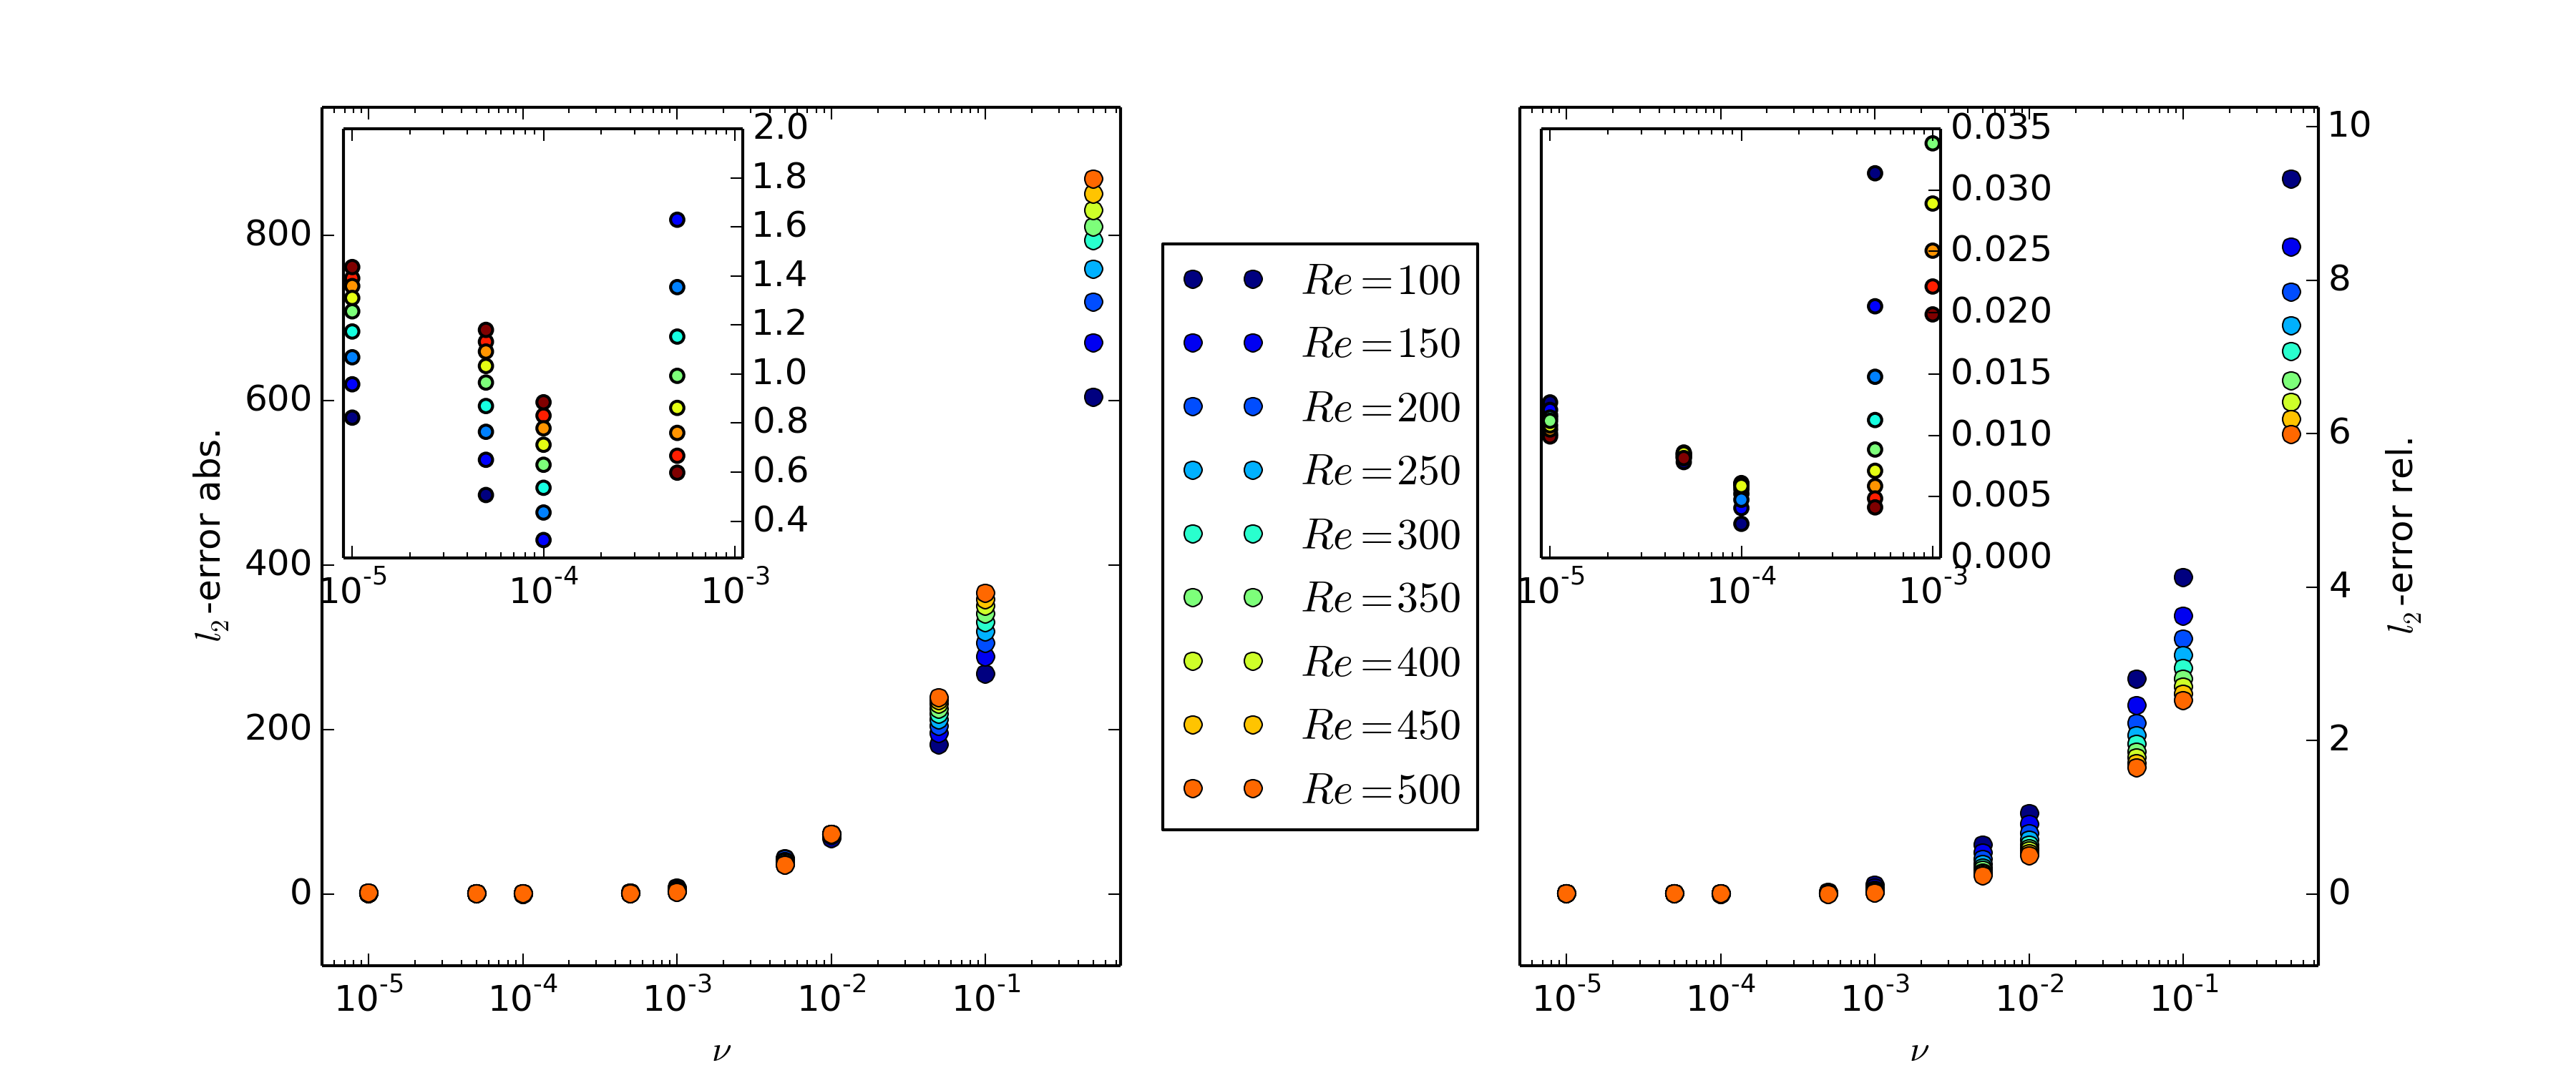
\includegraphics[width=1.0\textwidth]{gfx/immersed_boundary/2_vp/vp_error.png}\label{fig:vp_error}
  \caption{Absoluter und relativer Fehler in Abhängigkeit von Dämpfungskonsante $\nu$ und Reynoldszahl $Re$.}
\end{figure}

- for both error we can see a decrease until $\nu=1e-4$, followed by a slight increase as one can see in the inset
- what kind of decrease ?
- the behaviour will be clarified in the following grid convergence study
- the absolute error is growing with a decrease in the reynoldsnumber for $\nu>5\cdot10^{-3}$.
- this is as expected since the stress on the wall is larger, in the area

Betrachtet man den absoluten Fehler, so fällt auf das im Bereich , mit steigender Reynoldszahl, der Fehler zunimmt.
Dies entspricht zunächst der Erwartung, da das Geschwindigkeitsprofil mit steigender Reynoldszahl stärker an der Wand zerrt.
Allerdings kommt es im Bereich $\nu \in [1e-3 - 1e-2]$ zu einem umgekehrten Verhalten, der Fehler nimmt mit der Reynoldszahl ab,
Du Ursache hierfür liess sich nicht eindeutig klären.
Für den relativen Fehler lässt sich ein Abfall mit steigender Reynoldszahl beobachten. Da $\vec{f} \propto (\vec{v}-\vec{v_0})  \propto Re$ wird der Reibunsterm
proportional zur Reynoldszahl skaliert. Der Fehler durch den Rand ändert sich, im Vergleich zum Geschwindigskeitsprofil kaum, wodurch der Abfall zustande kommt.
Der relative Fehler fällt bei $\nu=1e-4=10\Delta t$ auf unter 1\%, wodurch dieser Wert als geeignet angesehen werden kann für zukünftige Simulationen mit der Volume-Penalization Methode.
-todo: fluktuation im rand bei vp?

-grid convergence study o2 and o4


\subsection{Direct Forcing Methode}
Während die Volume Penalization Methode die Geschwindigkeit ausserhalb des Volumens nicht vollständig auf Null setzt,
 kann dies durch eine implizite Berechnung des Dämpfungsterm erreichtwerden. Es stellt sich heraus das dieser Ansatz equivalent
  zu der Direct Forcing Methode ist, die erstmals von [] verwendet und in [] beschrieben wird.
Betrachten wir zunächst den diskretisierten Zeitschritt
\begin{align}
    \frac{\vec{u}^{n+1} -\vec{u}^n}{\Delta t} = \mathscr{L} + \vec{f}\\
\end{align}
wobei $\mathscr{L}$ den diskretiesierten Operatoren der PDE entspricht.
Für einen Punkt auf dem Rand des Volumens soll nun die Randbedingung $\vec{u}^{n+1} = \vec{u}_0$ eingehalten werden.
Mit Formel () folgt
\begin{align}
    \frac{\vec{u}_0 -\vec{u}^n}{\Delta t} = \mathscr{L} + \vec{f} \Rightarrow \vec{f} = \frac{\vec{u}_0 -\vec{u}^n}{\Delta t\cdot \mathscr{L}}\\
\end{align}

Mit der Annahme dass der Rand mit dem numerischen Gitter übereinstimmt ist es nicht nötig den Kraftterm zur berechnen, stattdessen lässt sich der
Schritt vereinfachen in dem der Randwert nach  jedem Zeitschritt direkt auf die gewünschte Randbedingung gesetzt wird. Durch die
implizite Behandlung kommt es zu keiner weiter Stabilitätsbedingung.
Analog zur Volume-Penalization Methode wurde eine Serie von Simulationen für eine planare Poiseuille-Strömung durchgeführt.
Das Setup enstpricht dem gleichen wie in Abschnitt (X), lediglich das Verfahren wurde entsprechend angepasst und es wurden finite Differenzen Verfahren zweiter und
vierter Ordnung getestet.
In Abbildung () ist der relative Fehler, im Vergleich zur Volume Penalization  Methode mit $\nu=1e-4$ dargestellt.
Für das Verfahren vierter Ordnung liegt der Fehler im Bereich von 1\% und ist im Mittel doppelt so groß wie für die Volume-Penalization Methode.
Der Fehler für das Verfahren zweiter Ordnung verschwindet hingegen nahezu.
Das Verhalten lässt sich durch die Verwendung unterschliedlicher Schablonen, wie in Abb() dargestellt,  der finiten differenzen Verfahren erklären.
Während das Verfahren zweiter Ordnung nur den Randpunkt sieht, liegt bei der vierten Ordnung ein Punkt innerhalb des Randes.
Da auch dieser Wert auf Null gesetzt wird, kommt es zu einem fehler in der Berechnung von $\nabla u$.

\begin{figure}[!tpb]
  \centering
Die Volume-Penalization Methode ermöglicht es, durch einen Kraftterm der auf die einzelnen Fluidzellen wirkt, mit wenig Aufwand Noslip-Ränder zu implementieren.
Das Verfahren wurde in mehreren Publikationen z.B. [bla] erfolgreich verwendet, eine mathematisch exaktere Abhandlung lässt sich z.B. in [bla2] finden.

\begin{wrapfigure}{r}{0.5\textwidth}
  \begin{center}
  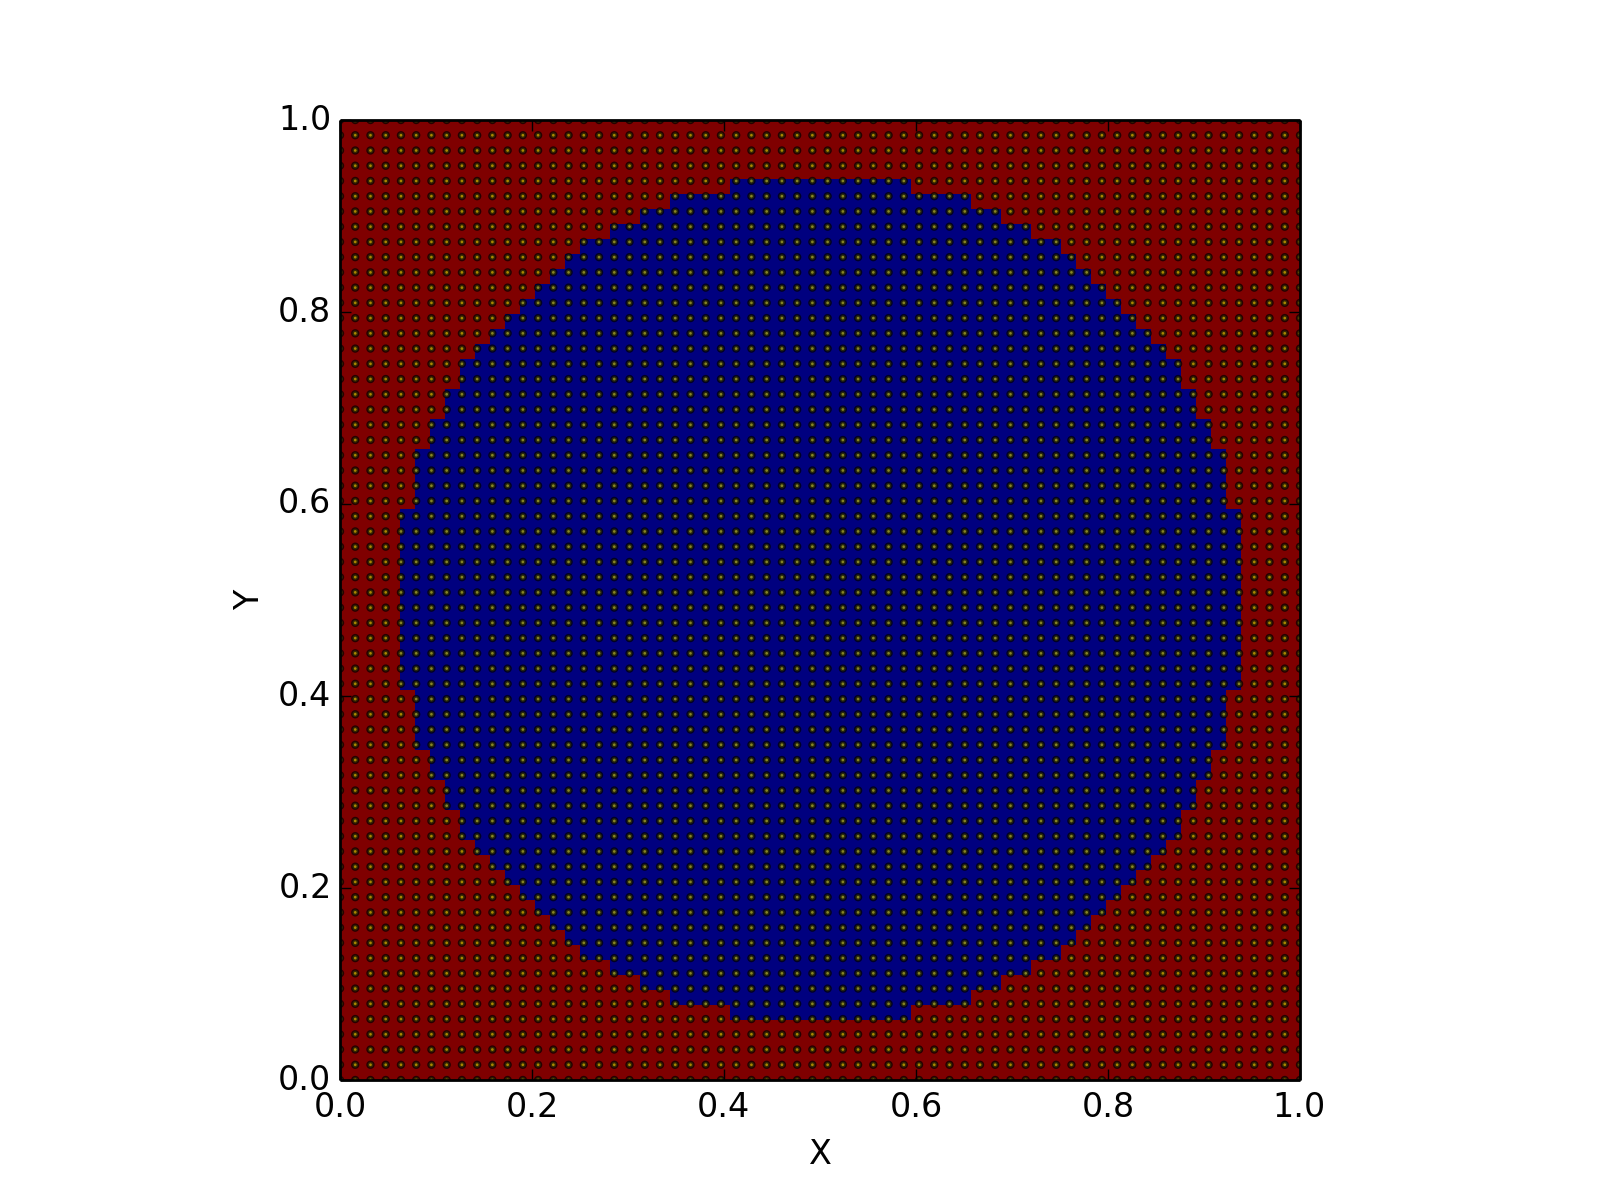
\includegraphics[width=0.5\textwidth]{gfx/immersed_boundary/mask.png}\label{fig:mask_vp}
  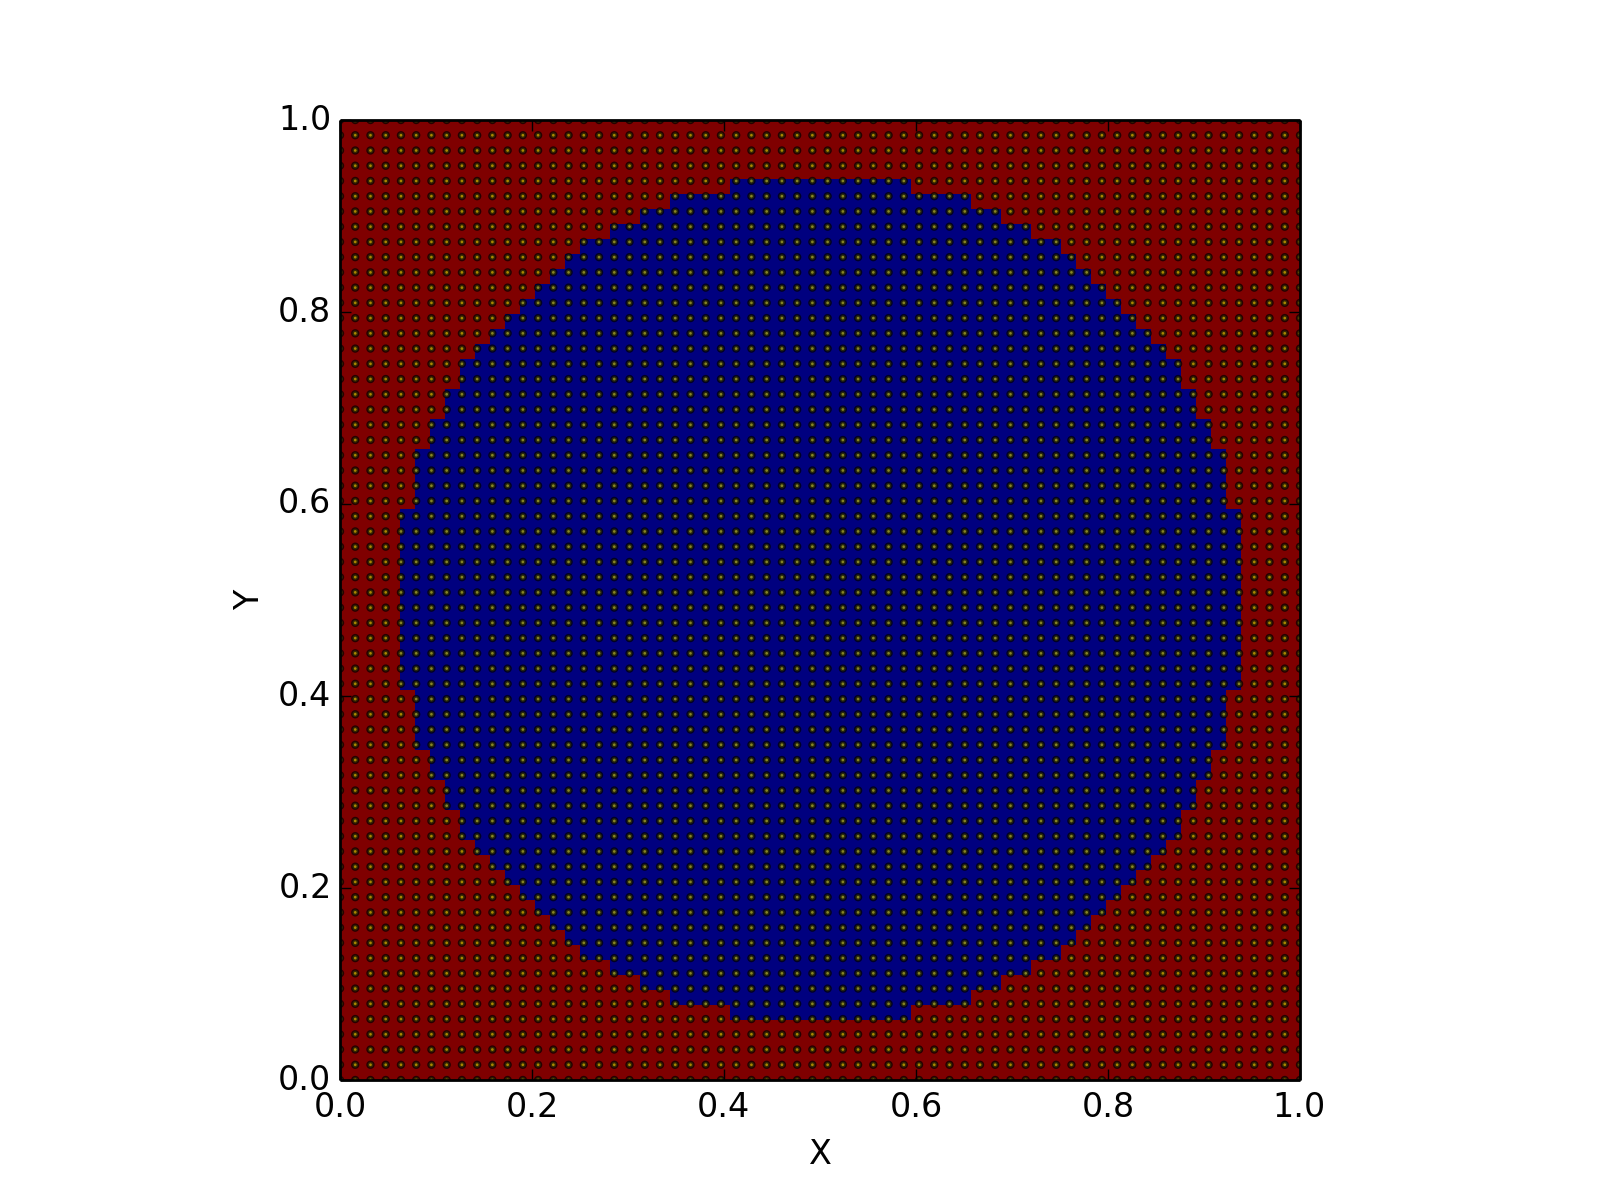
\includegraphics[width=0.5\textwidth]{gfx/immersed_boundary/mask.png}\label{fig:mask_vp}
  \end{center}
  \caption{Maskierungsfunktion $H(x,y,z=const.) = x^2 + y^2 < c$ für einen Zylinder. }
\end{wrapfigure}

Das Volumen wird zunächst in einen Fluidbereich und einen festen Wandbereich, wie in Abb.1 dargestellt, unterteilt. Für die Differenzierung der Bereiche während der Simulation wird  eine Maskierungsfunktion
\begin{align}
H(x, y, z) = \begin{cases}
                    0, & \text{für } \vec{x}(x,y,z) \in Fluid, \\
                    1, & \text{sonst}.
             \end{cases}
\end{align}
verwendet. Als zusätzlicher Kraftterm wird nun eine exponentielle Dämpfung eingeführt die nur auf den Wandbereich des Volumens wirkt.
\begin{align}
\vec{f} = \frac{H(x, y, z)}{\nu}(\vec{v} - \vec{v_0})
\end{align}
Bei $\vec{v_0}$ handelt es sich um die gewünschte Randbedingung, der Kraftterm ist also proportional zur Auslenkung $\vec{v}$ eines Punktes vom gewünschten Ruhezustand.
Die Antwort des Kraftterms wird durch die Dämpfungrate $\nu$ reguliert. Je kleiner $\nu$ desto stärker ist die Dämpfungsrate, allerdings kann der Term
nicht beliebig klein gesetzt werden da die Stabilität für $\nu < dt$ nicht mehr gewährleistet ist [source].
Da für die Lösung der der Geschwindingskeitsfelder mit der Methode der künstliche Kompressibilität  bereits ein sehr kleiner Zeitschritt verwendet wird (s.Abb. X)
kann im Vergleich zu anderen Verfahren wie z.B. (pseudo-spektrale) eine relativ starke Dämpfungsrate verwendet werden.

\subsubsection{Validierung mit MASA}
-validierung mit masa für alle verfahren oben.. cube /evtl zylinder?
-vegl. und argumentation ränder ehh auf null.
-ein beispiel mit vol.pen.

  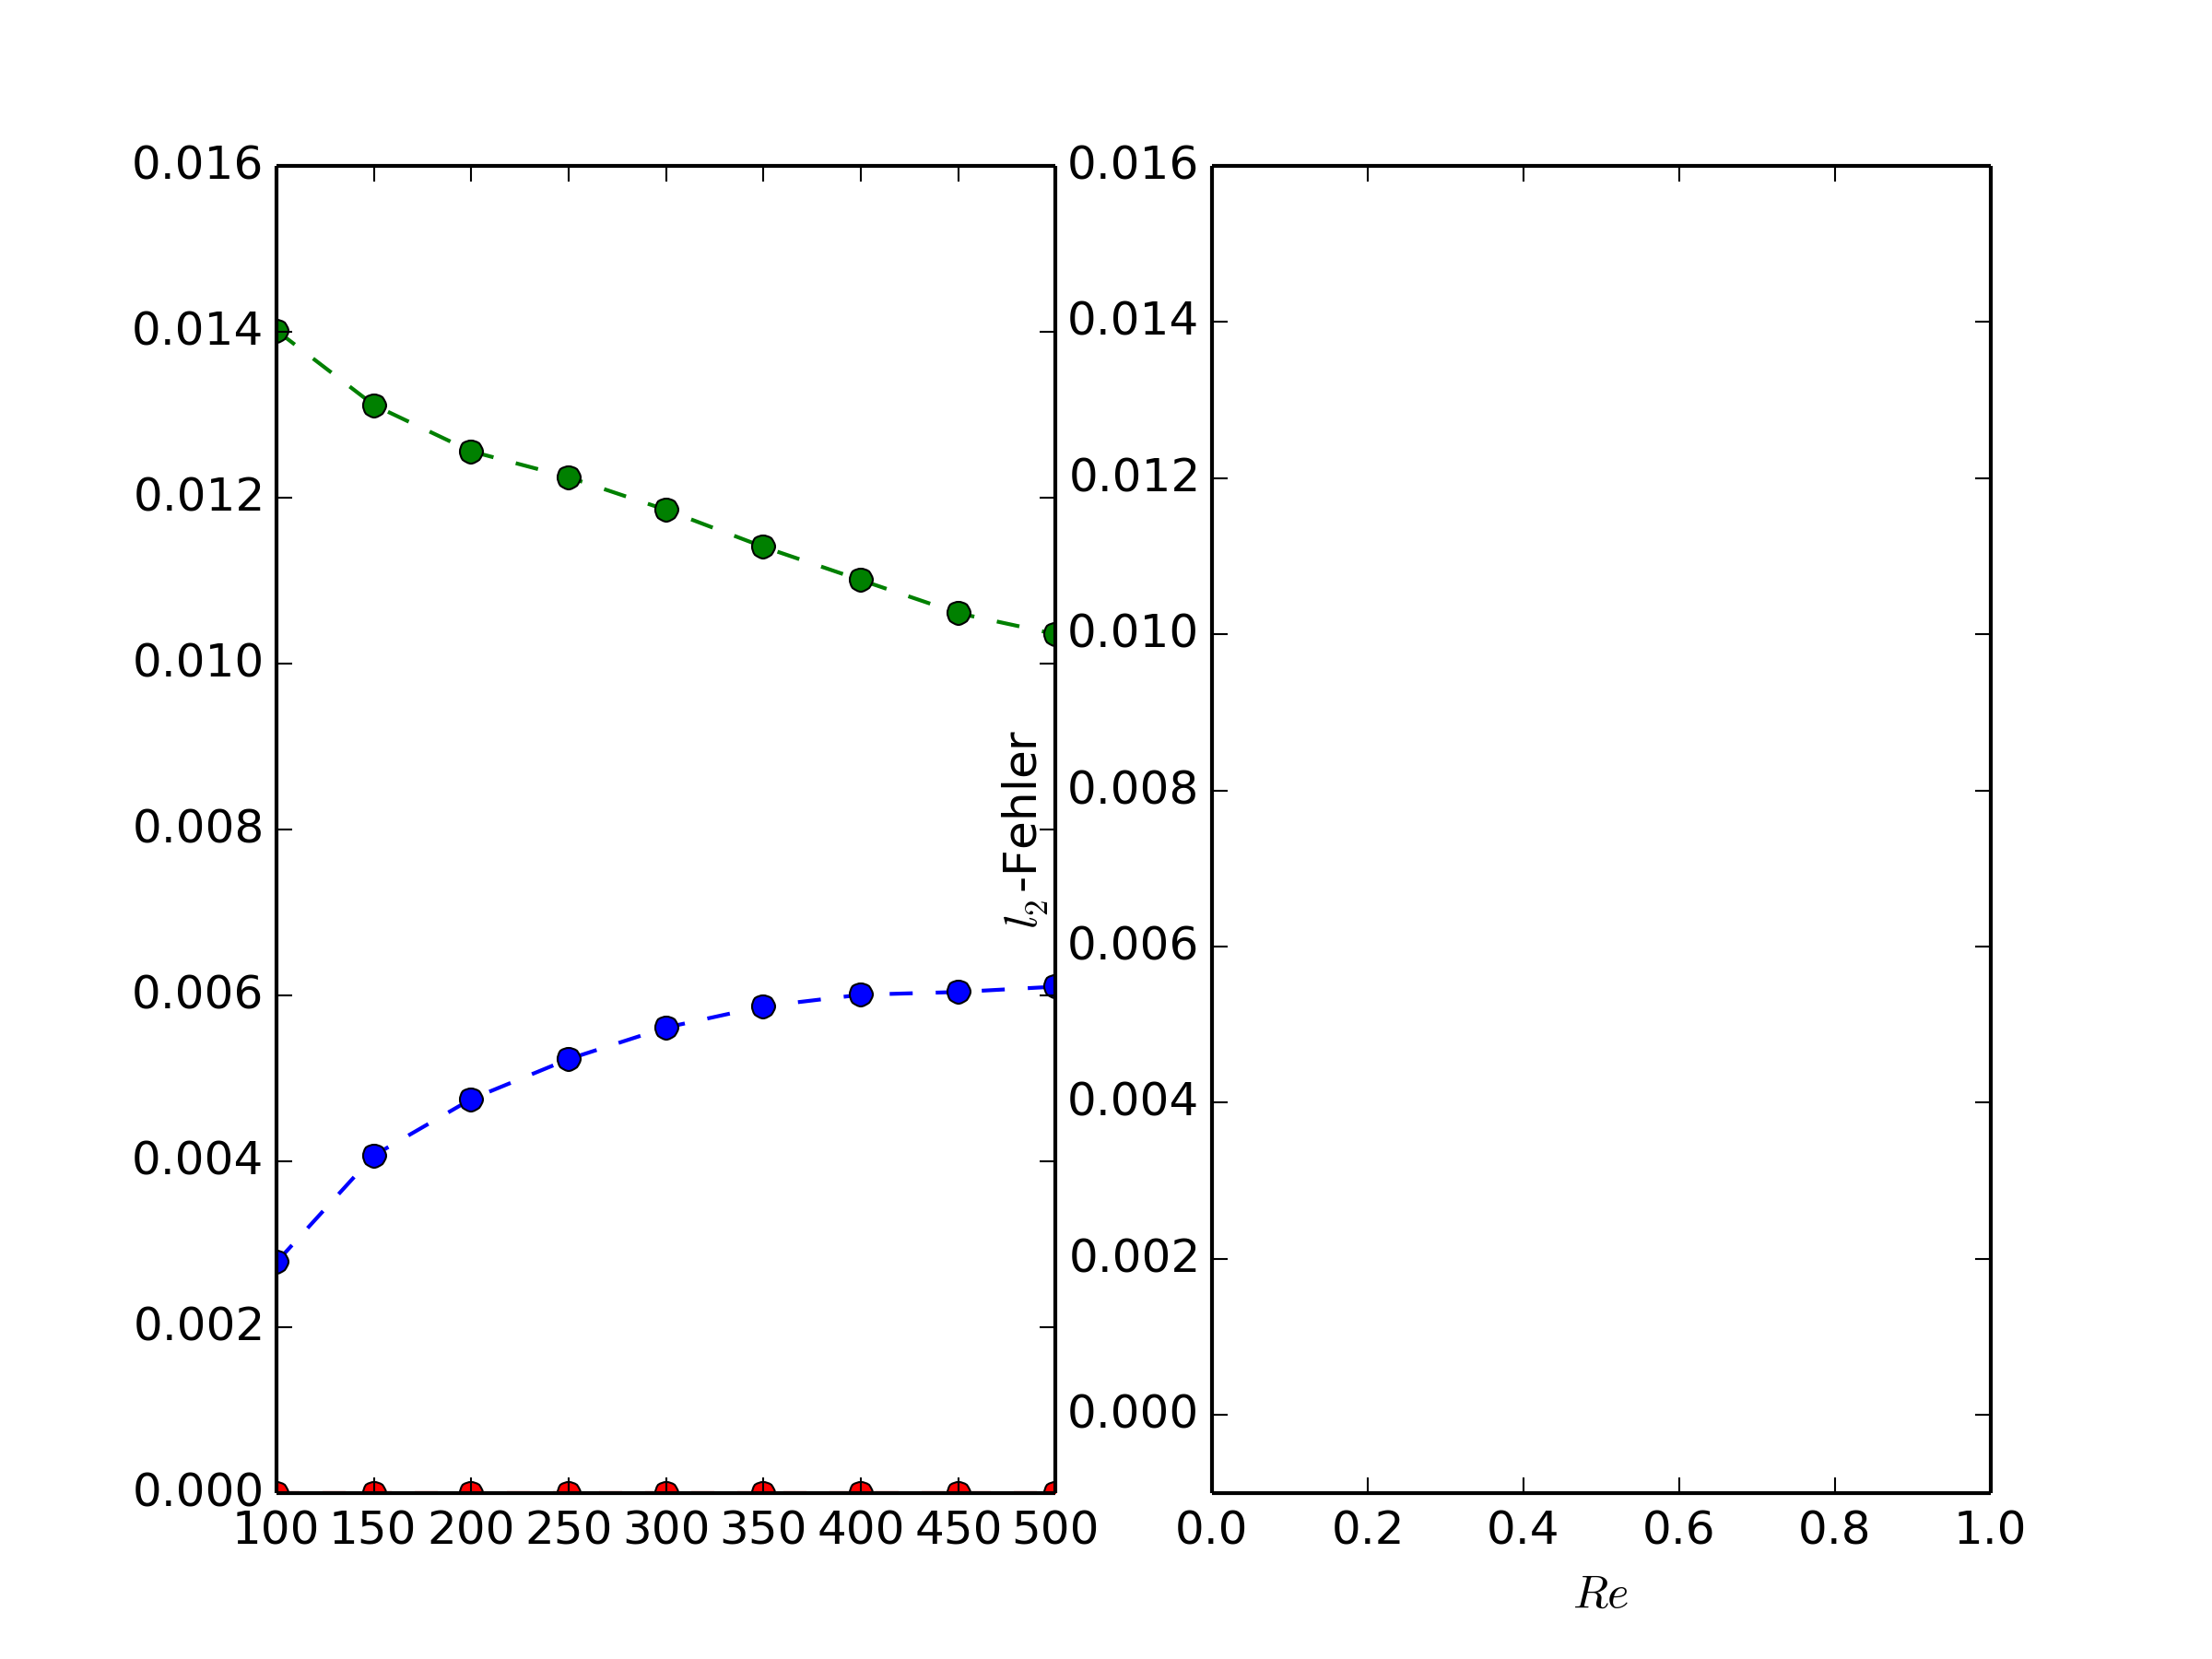
\includegraphics[width=0.6\textwidth]{gfx/immersed_boundary/dfo2o4.png}\label{fig:df_o2o4}
  \caption{bla}
\end{figure}

-Zeitserie

-einleitung gekrümmte geometrien

\subsection{Direct Forcing mit Volume Fraction}
-paper quote formeln
-implementierung beispiel

\section{Direct Forcing mit Interpolation}
-paper quote formeln
-implementierung beispiel

\section{Methoden-Vergleich und numerische Validierung}
In diesem Abschnitt sollen die verschiedenen Methoden über numerische Testfälle validiert und miteinnander
verglichen werden.


\subsubsection{Poiseuille Strömung im Zylinder}

\subsubsection{Zusammenfassung}


\subsection{No-Flux-Boundaries}

\subsubsection{'Variable Konduktivität'}










